\documentclass[11pt,ngerman,a4paper,]{article}
\usepackage{lmodern}

\usepackage{amssymb,amsmath}
\usepackage{tikz}
\usepackage{float}

\usepackage{enumitem}
\newlist{todolist}{itemize}{2}
\setlist[todolist]{label=$\square$}

\usepackage{ifxetex,ifluatex}
\usepackage{fixltx2e} % provides \textsubscript
\ifnum 0\ifxetex 1\fi\ifluatex 1\fi=0 % if pdftex
  \usepackage[T1]{fontenc}
  \usepackage[utf8]{inputenc}
\else % if luatex or xelatex
  \usepackage{unicode-math}
  \defaultfontfeatures{Ligatures=TeX,Scale=MatchLowercase}
\fi
% use upquote if available, for straight quotes in verbatim environments
\IfFileExists{upquote.sty}{\usepackage{upquote}}{}
% use microtype if available
\IfFileExists{microtype.sty}{%
\usepackage[]{microtype}
\UseMicrotypeSet[protrusion]{basicmath} % disable protrusion for tt fonts
}{}
\PassOptionsToPackage{hyphens}{url} % url is loaded by hyperref
\usepackage[unicode=true]{hyperref}
\hypersetup{
            pdftitle={Stromprognose mittels Self Learning Activation Functions \& Liquid Neuronal Networks},
            pdfkeywords={SLAF, LNN, Forecasting, Electric Power},
            pdfborder={0 0 0},
            breaklinks=true}
\urlstyle{same}  % don't use monospace font for urls
\usepackage{geometry}
\geometry{left=2.5cm,right=2.5cm,top=2.5cm,bottom=2.5cm}
\ifnum 0\ifxetex 1\fi\ifluatex 1\fi=0 % if pdftex
  \usepackage[shorthands=off,main=ngerman]{babel}
\else
  \usepackage{polyglossia}
  \setmainlanguage[]{}
\fi
\usepackage[style=authoryear-comp,]{biblatex}
\addbibresource{references.bib}
\usepackage{color}
\usepackage{fancyvrb}
\newcommand{\VerbBar}{|}
\newcommand{\VERB}{\Verb[commandchars=\\\{\}]}
\DefineVerbatimEnvironment{Highlighting}{Verbatim}{commandchars=\\\{\}}
% Add ',fontsize=\small' for more characters per line
\usepackage{framed}
\definecolor{shadecolor}{RGB}{248,248,248}
\newenvironment{Shaded}{\begin{snugshade}}{\end{snugshade}}
\newcommand{\AlertTok}[1]{\textcolor[rgb]{0.94,0.16,0.16}{#1}}
\newcommand{\AnnotationTok}[1]{\textcolor[rgb]{0.56,0.35,0.01}{\textbf{\textit{#1}}}}
\newcommand{\AttributeTok}[1]{\textcolor[rgb]{0.13,0.29,0.53}{#1}}
\newcommand{\BaseNTok}[1]{\textcolor[rgb]{0.00,0.00,0.81}{#1}}
\newcommand{\BuiltInTok}[1]{#1}
\newcommand{\CharTok}[1]{\textcolor[rgb]{0.31,0.60,0.02}{#1}}
\newcommand{\CommentTok}[1]{\textcolor[rgb]{0.56,0.35,0.01}{\textit{#1}}}
\newcommand{\CommentVarTok}[1]{\textcolor[rgb]{0.56,0.35,0.01}{\textbf{\textit{#1}}}}
\newcommand{\ConstantTok}[1]{\textcolor[rgb]{0.56,0.35,0.01}{#1}}
\newcommand{\ControlFlowTok}[1]{\textcolor[rgb]{0.13,0.29,0.53}{\textbf{#1}}}
\newcommand{\DataTypeTok}[1]{\textcolor[rgb]{0.13,0.29,0.53}{#1}}
\newcommand{\DecValTok}[1]{\textcolor[rgb]{0.00,0.00,0.81}{#1}}
\newcommand{\DocumentationTok}[1]{\textcolor[rgb]{0.56,0.35,0.01}{\textbf{\textit{#1}}}}
\newcommand{\ErrorTok}[1]{\textcolor[rgb]{0.64,0.00,0.00}{\textbf{#1}}}
\newcommand{\ExtensionTok}[1]{#1}
\newcommand{\FloatTok}[1]{\textcolor[rgb]{0.00,0.00,0.81}{#1}}
\newcommand{\FunctionTok}[1]{\textcolor[rgb]{0.13,0.29,0.53}{\textbf{#1}}}
\newcommand{\ImportTok}[1]{#1}
\newcommand{\InformationTok}[1]{\textcolor[rgb]{0.56,0.35,0.01}{\textbf{\textit{#1}}}}
\newcommand{\KeywordTok}[1]{\textcolor[rgb]{0.13,0.29,0.53}{\textbf{#1}}}
\newcommand{\NormalTok}[1]{#1}
\newcommand{\OperatorTok}[1]{\textcolor[rgb]{0.81,0.36,0.00}{\textbf{#1}}}
\newcommand{\OtherTok}[1]{\textcolor[rgb]{0.56,0.35,0.01}{#1}}
\newcommand{\PreprocessorTok}[1]{\textcolor[rgb]{0.56,0.35,0.01}{\textit{#1}}}
\newcommand{\RegionMarkerTok}[1]{#1}
\newcommand{\SpecialCharTok}[1]{\textcolor[rgb]{0.81,0.36,0.00}{\textbf{#1}}}
\newcommand{\SpecialStringTok}[1]{\textcolor[rgb]{0.31,0.60,0.02}{#1}}
\newcommand{\StringTok}[1]{\textcolor[rgb]{0.31,0.60,0.02}{#1}}
\newcommand{\VariableTok}[1]{\textcolor[rgb]{0.00,0.00,0.00}{#1}}
\newcommand{\VerbatimStringTok}[1]{\textcolor[rgb]{0.31,0.60,0.02}{#1}}
\newcommand{\WarningTok}[1]{\textcolor[rgb]{0.56,0.35,0.01}{\textbf{\textit{#1}}}}
\usepackage{longtable,booktabs}
% Fix footnotes in tables (requires footnote package)
\IfFileExists{footnote.sty}{\usepackage{footnote}\makesavenoteenv{long table}}{}

\IfFileExists{parskip.sty}{%
\usepackage{parskip}
}{% else
\setlength{\parindent}{0pt}
\setlength{\parskip}{6pt plus 2pt minus 1pt}
}
\setlength{\emergencystretch}{3em}  % prevent overfull lines
\providecommand{\tightlist}{%
  \setlength{\itemsep}{0pt}\setlength{\parskip}{0pt}}
\setcounter{secnumdepth}{5}

% set default figure placement to htbp
\makeatletter
\def\fps@figure{htbp}
\makeatother


\title{Stromprognose mittels Self Learning Activation Functions \& Liquid Neuronal Networks}

%% MONASH STUFF

%% CAPTIONS
\RequirePackage{caption}
\DeclareCaptionStyle{italic}[justification=centering]
 {labelfont={bf},textfont={it},labelsep=colon}
\captionsetup[figure]{style=italic,format=hang,singlelinecheck=true}
\captionsetup[table]{style=italic,format=hang,singlelinecheck=true}

%% FONT
\RequirePackage{bera}
\RequirePackage{mathpazo}

%% HEADERS AND FOOTERS
\RequirePackage{fancyhdr}
\pagestyle{fancy}
\rfoot{\Large\sffamily\raisebox{-0.1cm}{\textbf{\thepage}}}
\makeatletter
\lhead{\textsf{\expandafter{\@title}}}
\makeatother
\rhead{}
\cfoot{}
\setlength{\headheight}{15pt}
\renewcommand{\headrulewidth}{0.4pt}
\renewcommand{\footrulewidth}{0.4pt}
\fancypagestyle{plain}{%
\fancyhf{} % clear all header and footer fields
\fancyfoot[C]{\sffamily\thepage} % except the center
\renewcommand{\headrulewidth}{0pt}
\renewcommand{\footrulewidth}{0pt}}

%% MATHS
\RequirePackage{bm,amsmath}
\allowdisplaybreaks

%% GRAPHICS
\RequirePackage{graphicx}
\setcounter{topnumber}{2}
\setcounter{bottomnumber}{2}
\setcounter{totalnumber}{4}
\renewcommand{\topfraction}{0.85}
\renewcommand{\bottomfraction}{0.85}
\renewcommand{\textfraction}{0.15}
\renewcommand{\floatpagefraction}{0.8}

%\RequirePackage[section]{placeins}

%% SECTION TITLES
\RequirePackage[compact,sf,bf]{titlesec}
\titleformat{\section}[block]
  {\fontsize{15}{17}\bfseries\sffamily}
  {\thesection}
  {0.4em}{}
\titleformat{\subsection}[block]
  {\fontsize{12}{14}\bfseries\sffamily}
  {\thesubsection}
  {0.4em}{}
\titlespacing{\section}{0pt}{*5}{*1}
\titlespacing{\subsection}{0pt}{*2}{*0.2}


%% TITLE PAGE
\def\Date{\number\day}
\def\Month{\ifcase\month\or
 January\or February\or March\or April\or May\or June\or
 July\or August\or September\or October\or November\or December\fi}
\def\Year{\number\year}

\makeatletter
\def\wp#1{\gdef\@wp{#1}}\def\@wp{??/??}
\def\jel#1{\gdef\@jel{#1}}\def\@jel{??}
\def\showjel{{\large\textsf{\textbf{JEL classification:}}~\@jel}}
\def\nojel{\def\showjel{}}
\def\addresses#1{\gdef\@addresses{#1}}\def\@addresses{??}
\def\cover{{\sffamily\setcounter{page}{0}
        \thispagestyle{empty}
        \placefig{2}{1.5}{width=5cm}{FHSWF}
        %\placefig{16.9}{1.5}{width=2.1cm}{MBusSchool}
        %\begin{textblock}{4}(16.9,4)ISSN 1440-771X\end{textblock}
        \begin{textblock}{7}(12.7,27.9)\hfill
        
\includegraphics[height=1cm]{WirGebenImpulse}~~~
        %\includegraphics[height=0.7cm]{EQUIS}~~~
        %\includegraphics[height=0.7cm]{AMBA}
        \end{textblock}
        \vspace*{0.5cm}
        \begin{center}\Large
                  Fachhochschule Südwestfalen\\
          Fachbereich Ingenieur- und Wirtschaftswissenschaften\\[.5cm]
                %%
         Neuronal Network and Deep Learning (Prof.~Dr.~Thomas Kopinski und Felix Neubürger) \\ 
        \normalsize   Gutachter: Prof.~Dr.~Thomas Kopinski und Felix Neubürger   
        %%
        \end{center}\vspace{1cm}
        \begin{center}
        \fbox{\parbox{14cm}{\begin{onehalfspace}\centering\huge\vspace*{0.2cm}
                \textsf{\textbf{\expandafter{\@title}}}\vspace{1cm}\par
                \LARGE\@author\end{onehalfspace}
        }}
        %%
        %%
        \end{center}
        %%
        \vspace{2cm}
                \begin{singlespace}
        \begin{abstract}
        \footnotesize
        Bei der Vorhersage von Zeitreihen kann die Anpassung an die aktuelle Situation eine große Rolle spielen. So i.d.r. ob z.B. Umwelteinflüsse oder Pandemien eine große Veränderung in einer Zeitreihe herbeiführen. Der erste Ansatz für eine Vorhersage von Zeitreihen basiert in dieser Arbeit auf den Liquid Neuronal Networks (LNN). Die LNNs sind dynamisch und passen sich an die aktuelle Situation an, lernen also immer weiter. Als eine Ergänzung zu den LNNs wir die Self Learning Activation Function (SLAF) implementiert. Diese approximiert die Parametrierung der richtigen Aktivierungsfunktion. Das Neuronale Netz wird auf den Datensatz der Stromerzeugung in den Jahren 2004-2018 vom Unternehmen American Electric Power angewandt.
        \end{abstract}
        \end{singlespace}
                        \begin{keywords}
        \footnotesize
        SLAF, LNN, Forecasting, Electric Power
        \end{keywords}
                %%
        \vfill
                \begin{center}
                \footnotesize
                Meschede\linebreak
                \today
        \end{center}\vspace*{0.5cm}}}
\def\pageone{{\sffamily\setstretch{1}%
        \thispagestyle{empty}%
        \vbox to \textheight{%
                {\fontsize{24.88}{30}\sffamily\textbf{\expandafter{Ehrenwörtliche Erklärung}}}
        \vspace{1cm}\par
        Ich erkläre hiermit ehrenwörtlich, dass ich die vorliegende Arbeit selbständig angefertigt habe. Die aus fremden Quellen direkt und indirekt übernommenen Gedanken sind als solche kenntlich gemacht. Die Arbeit wurde weder einer anderen Prüfungsbehörde vorgelegt noch veröffentlicht.\\\\
        Ich weiß, dass die Arbeit in digitalisierter Form daraufhin überprüft werden kann, ob unerlaubte Hilfsmittel verwendet wurden und ob es sich – insgesamt oder in Teilen – um ein Plagiat handelt. Zum Vergleich meiner Arbeit mit existierenden Quellen darf sie in eine Datenbank eingestellt werden und nach der Überprüfung zum Vergleich mit künftig eingehenden Arbeiten dort verbleiben.\\
                \begin{flushright} Meschede, \today. \end{flushright}
        \vspace{1cm}\par
        \raggedright\baselineskip=1.2cm
        \hspace{1cm}\parbox{14cm}{\sffamily\large\@addresses}\vspace{1cm}\vfill
%        \hspace{1cm}{\large\Date~\Month~\Year}\\[1cm]
%        \hspace{1cm}\showjel\vss
                  \footnotesize \center Diese Erklärung ist nur mit der Unterschrift aller Autoren gültig.
                    }}}

\def\blindtitle{{\sffamily
     \thispagestyle{plain}\raggedright\baselineskip=1.2cm
     {\fontsize{24.88}{30}\sffamily\textbf{\expandafter{\@title}}}\vspace{1cm}\par
        }}

\def\pagetwo{{\sffamily\setstretch{0.8}%
  \thispagestyle{empty}%
  \vbox to \textheight{%
          {\fontsize{24.88}{30}\sffamily\textbf{\expandafter{Checkliste}}}
    \vspace{0.7cm}\par

    \textbf{Ich erkläre hiermit, dass in der vorliegenden Arbeit\dots} \\

  \textbf{\ldots folgende inhaltliche Kriterien im Hinblick auf die Forschungsfrage erfüllt sind:}
      \begin{todolist}
      \setlength\itemsep{-0.3em}
      \item Die Arbeit enthält (mindestens) eine eindeutig formulierte Forschungsfrage.
      \item Alle Forschungsfrage(n) werden im Schlussteil der Arbeit umfänglich beantwortet.
      \item Verwendete (analytische) Verfahren tragen erkennbar zur Beantwortung der aufgeworfenen Forschungsfrage bei und sind eindeutig damit verknüpft.
      \item Alle verwendeten Variablen sind beschrieben, sodass keine Variablen analysiert werden, die nicht beschrieben wurden. Alle beschriebenen Variablen werden für das Nachvollziehen der Argumentation benötigt.
      \end{todolist}

    \textbf{\ldots  bei der Ergebnisdarstellung Folgendes beachtet wird:}
      \begin{todolist}
      \setlength\itemsep{-0.3em}
      \item Formeln der Lehrunterlagen (Folien, Skripte, Studienbuch) werden in der Arbeit nicht wiederholt. Eigene Rechnungen (z.B. zur Generierung neuer Variablen) werden mit eigenen Formeln dargestellt.
      \item Die Arbeit enthält keine "Rechenrezepte", d.h. jede Rechnung ist nachvollziehbar dargestellt.
      \item Tabellen- und Abbildungen sind beschriftet und enden mit einem Punkt.
      \item Jede in der Arbeit enthaltene Abbildung und Tabelle ist auch in Textform beschrieben, erläutert und interpretiert und auf diese wird an der entsprechenden Stelle im Text verwiesen. Abbildungen und Tabellen ergänzen die textuelle Darstellung und substituieren sie nicht.
      \item Keine Abbildung ist ein Tortendiagramm.
      \item Aufgelistete Zahlen folgen der in R verwendeten Notation und nutzen einen Punkt als Dezimaltrennzeichen (Alle Zahlen sind einheitlich formatiert).
      \item Dargestellte Ergebnisse weisen 4 Nachkommastellen aus.
      \item In der Arbeit genannte Zahlen sind mitsamt deren Einheiten aufgeführt.
      \item Handschriftliche Ergänzungen, Rechnungen und Zeichnungen werden nicht bewertet. Nutzen Sie für die Darstellung von Rechnungen die LaTeX-Notation in RMarkdown. Ersetzen Sie handschriftliche Zeichnungen durch z.B. in R erzeugte Diagramme.
      \end{todolist}

  \textbf{\ldots die Sprache wie folgt gestaltet ist:}
      \begin{todolist}
      \setlength\itemsep{-0.3em}
      \item Die Arbeit ist frei von ausschmückenden Sprachkonstrukten, sodass der Fokus der textuellen Darstellung auf dem Untersuchungsgegenstand (nicht der sprachlichen Ausgestaltung) liegt (Academic Rigor).
       \item Die Arbeit enthält keine Formulierungen, bei denen Sie sich nicht entscheiden konnten (Häufig durch Striche "/"  im Text gekennzeichnet).
      \item Die Arbeit ist frei von Worten, die Präzision vorgeben ohne  Präzise zu sein (z.B. verschiedene, manche, bestimmte Zeitpunkte).
      \item Verzichten Sie insb. in der Inhaltsdarstellung auf Modalverben (insb. sollen;  Anstelle von "In dieser Arbeit soll..." --> "In dieser Arbeit wird...")
      \item Die Aussagen im Text enthalten wenig bis keine Superlative, enthaltene Superlative (= Behauptungen) sind mit wissenschaftlichen (!) Quellen belegt.
      \end{todolist}



    \textbf{\ldots weiterhin Folgendes erfüllt ist:}
      \begin{todolist}
      \setlength\itemsep{-0.3em}
      \item Einzelne Sätze konstituieren keine Absätze. Jeder Absatz besteht aus mehreren Sätzen. Absätze bilden inhaltliche Einheiten.
      \item Jede Untergliederungsebene enthält mindestens zwei Einträge (z.B. Kapitel 3.1 kann es nur geben, wenn es auch Kapitel 3.2 gibt).
      \item Alle Quellen im Literaturverzeichnis werden in der Arbeit verwendet. Alle in der Arbeit verwendeten Quellenangaben sind im Literaturverzeichnis enthalten.
      \item Alle Autoren haben die Ehrenwörtliche Erklärung eigenhändig unterschrieben.
      \end{todolist}

        \vfill
          \footnotesize \center Alle Listeneinträge müssen geprüft werden.
      }}}

%\def\titlepage{{\cover\newpage\pageone\newpage\blindtitle}}
\def\titlepage{{\cover\newpage\pageone}}


\def\blind{\def\titlepage{{\blindtitle}}\let\maketitle\blindtitle}
\def\titlepageonly{\def\titlepage{{\pageone\end{document}}}}
\def\nocover{\def\titlepage{{\pageone\newpage\blindtitle}}\let\maketitle\titlepage}
\let\maketitle\titlepage
\makeatother

%% SPACING
\RequirePackage{setspace}
\newcommand{\codespacing}{\spacing{1}}
\newcommand{\textspacing}{\spacing{1.25}}
\usepackage{etoolbox}
\makeatletter
\preto{\@verbatim}{\partopsep=-5pt}
\makeatother
\setlist[itemize]{topsep=0pt, parsep=5pt}

\textspacing
%\spacing{1.5}

%% LINE AND PAGE BREAKING
\sloppy
\clubpenalty = 10000
\widowpenalty = 10000
\brokenpenalty = 10000
\RequirePackage{microtype}

%% PARAGRAPH BREAKS
\setlength{\parskip}{1.4ex}
\setlength{\parindent}{0em}

%% HYPERLINKS
\RequirePackage{xcolor} % Needed for links
\definecolor{darkblue}{rgb}{0,0,.6}
\RequirePackage{url}

\makeatletter
\@ifpackageloaded{hyperref}{}{\RequirePackage{hyperref}}
\makeatother
\hypersetup{
     citecolor=0 0 0,
     breaklinks=true,
     bookmarksopen=true,
     bookmarksnumbered=true,
     linkcolor=darkblue,
     urlcolor=blue,
     citecolor=darkblue,
     colorlinks=true}

%% KEYWORDS
\newenvironment{keywords}{\par\vspace{0.5cm}\noindent{\sffamily\textbf{Keywords:}}}{\vspace{0.25cm}\par\hrule\vspace{0.5cm}\par}

%% ABSTRACT
\renewenvironment{abstract}{\begin{minipage}{\textwidth}\parskip=1.4ex\noindent
\hrule\vspace{0.1cm}\par{\sffamily\textbf{\abstractname}}\newline}
  {\end{minipage}}


\usepackage[T1]{fontenc}
\usepackage[utf8]{inputenc}

\usepackage[showonlyrefs]{mathtools}
\usepackage[no-weekday]{eukdate}

%% BIBLIOGRAPHY

\makeatletter
\@ifpackageloaded{biblatex}{}{\usepackage[style=authoryear-comp, backend=biber, natbib=true]{biblatex}}
\makeatother
\ExecuteBibliographyOptions{bibencoding=utf8,minnames=1,maxnames=3, maxbibnames=99,dashed=false,terseinits=true,giveninits=true,uniquename=false,uniquelist=false,doi=false, isbn=false,url=true,sortcites=false}

\DeclareFieldFormat{url}{\texttt{\url{#1}}}
\DeclareFieldFormat[article]{pages}{#1}
\DeclareFieldFormat[inproceedings]{pages}{\lowercase{pp.}#1}
\DeclareFieldFormat[incollection]{pages}{\lowercase{pp.}#1}
\DeclareFieldFormat[article]{volume}{\mkbibbold{#1}}
\DeclareFieldFormat[article]{number}{\mkbibparens{#1}}
\DeclareFieldFormat[article]{title}{\MakeCapital{#1}}
\DeclareFieldFormat[inproceedings]{title}{#1}
\DeclareFieldFormat{shorthandwidth}{#1}
% No dot before number of articles
\usepackage{xpatch}
\xpatchbibmacro{volume+number+eid}{\setunit*{\adddot}}{}{}{}
% Remove In: for an article.
\renewbibmacro{in:}{%
  \ifentrytype{article}{}{%
  \printtext{\bibstring{in}\intitlepunct}}}

\makeatletter
\DeclareDelimFormat[cbx@textcite]{nameyeardelim}{\addspace}
\makeatother
\renewcommand*{\finalnamedelim}{%
  %\ifnumgreater{\value{liststop}}{2}{\finalandcomma}{}% there really should be no funny Oxford comma business here
  \addspace\&\space}


\nojel

\RequirePackage[absolute,overlay]{textpos}
\setlength{\TPHorizModule}{1cm}
\setlength{\TPVertModule}{1cm}
\def\placefig#1#2#3#4{\begin{textblock}{.1}(#1,#2)\rlap{\includegraphics[#3]{#4}}\end{textblock}}




\author{Vitali~Krilov, Vladislav~Stasenko}
\addresses{\textbf{Vitali Krilov}\newline
MatNr: 30329089
\newline{Email: \href{mailto:krilov.vitali@fh-swf.de}{\nolinkurl{krilov.vitali@fh-swf.de}}}\newline Corresponding Author\\[1cm]
\textbf{Vladislav Stasenko}\newline
MatNr: 87654321
\newline{Email: \href{mailto:stasenko.vladislav@fh-swf.de}{\nolinkurl{stasenko.vladislav@fh-swf.de}}}\\[1cm]
}

\date{\sf\Date.~\Month~\Year}
\makeatletter
 \lfoot{\sf Krilov, Stasenko: \@date}
\makeatother

\usepackage{hyperref}
\usepackage{caption}
\usepackage{csquotes}
\usepackage{graphicx}
\usepackage{microtype}
\usepackage{tabularx}
\usepackage{longtable}


\begin{document}
\maketitle
% % \begin{abstract}
% Bei der Vorhersage von Zeitreihen kann die Anpassung an die aktuelle Situation eine große Rolle spielen. So i.d.r. ob z.B. Umwelteinflüsse oder Pandemien eine große Veränderung in einer Zeitreihe herbeiführen. Der erste Ansatz für eine Vorhersage von Zeitreihen basiert in dieser Arbeit auf den Liquid Neuronal Networks (LNN). Die LNNs sind dynamisch und passen sich an die aktuelle Situation an, lernen also immer weiter. Als eine Ergänzung zu den LNNs wir die Self Learning Activation Function (SLAF) implementiert. Diese approximiert die Parametrierung der richtigen Aktivierungsfunktion. Das Neuronale Netz wird auf den Datensatz der Stromerzeugung in den Jahren 2004-2018 vom Unternehmen American Electric Power angewandt.
% \end{abstract}
% % % \begin{keywords}
% SLAF, LNN, Forecasting, Electric Power
% \end{keywords}
% 
{
\newpage
\setcounter{tocdepth}{2}
\tableofcontents
\newpage
}
\listoffigures
\newpage
\section{Einleitung}\label{einleitung}

Geht es um Vorhersagen von Zeitreihen mit komplexen saisonalen Mustern, so sind wohl die bekanntesten statistischen Modellierungen Autoregressive Integrated Moving Average (ARIMA), Exponential Smoothing oder das Prophet-Modell. Im Bereich der neuronalen Netze ist Long-Short-Term-Memory (LSTM), welches eine spezielle Art von Recurrent Neural Network RNN ist, das bekannte neuronale Netz für komplexe Zeitreihen. Ein aktuell neuer Ansatz für eine Vorhersage von komplexen Zeitreihen ist ein weiteres RNN, das Liquid Time-Constant Neuronal Network oder kurz Liquid Neuronal Network (LNN). Es geht darum, mit weniger Rechenleistung und geringerem Datensatz ein kompakteres Modell zu erzeugen, welches sich z.B. in Echtzeit an die Datenlage anpassen kann. So kann z.B. ein LSTM 100.000 - 1.000.000 Parameter haben, wobei das LNN mit bis zu 10.000 Parametern auskommt und ähnliche Resultate liefert. So ist eine Anbindung an elektronische Messgeräte oder Raspberry Pi mit weniger Rechenleistung im Gegensatz zu LSTM möglich. In dieser Arbeit wird ein LNN auf einen Datensatz von der Stromerzeugung vom Unternehmen American Electric Power angewandt. Das Ziel ist es, eine Vorhersage für den nächsten Tag ``day-ahead'' zu treffen. Bei den neuronalen Netzen steht immer die Frage im Raum, welche Aktivierungsfunktion genutzt werden soll. Als Ergänzung zu dem LNN wird ein self learning activation function (SLAF) Modell implementiert. SLAF soll das vanishing gradient Problem dezimieren, aber auch eine approximierte Aktivierungsfunktion für das LNN finden.

Um den roten Faden besser folgen zu können, werden die einzelnen Kapitel kurz erläutert:

\textbf{Methodik:} Im Kapitel der Methodik wird auf die theoretischen Grundlagen eingegangen. Im ersten Abschnitt wird auf die Liquid Time-Constant Neuronal Networks (LTCNNs) eingegangen. Hier wird beschrieben, was ein LTCNN ist und wie die mathematische Zusammensetzung aussieht. Der Begriff ``Luquid'' und das Lernverhalten wird in Bezug auf das neuronale Netz erläutert.

Darauf folgt die Erklärung, was eine Self Learnable Activation FUnction (SLAF) ist. Es wird auf das Konzept hinter SLAFs prägnant eingegangen und erläutert. Der Begriff der swish-Funktion wird eingeführt und beschrieben.

Als Letztes wird vollständigkeitshalber auf das Auto Regressive-Moving Average (ARIMA), das Prophet-Modell und die verwendeten Metriken eingegangen.

\textbf{Datengrundlage und Datenanalyse:} Im Kapitel der Datengrundlage und Datenanalyse wird auf den verwendeten Datensatz eingegangen. Dieser wird in seiner Rohform präsentiert und daraufhin analytisch untersucht. Dabei wird auf Datenkonsistenz (fehlende Werte und doppelte Beobachtungen) eingegangen. Das Verfahren zur Interpolation der fehlenden Daten und der Umgang mit doppelten Beobachtungen wird erläutert. Daraufhin wird der gesäuberte Datensatz in Bezug auf das Jahr, Woche und Stunde untersucht. Gegen Ende wird auf den Effekt der Feiertage eingegangen und es werden Features generiert, die in das neuronale Netz einfließen sollen.

\textbf{Implementierung:} Im Kapitel der Implementierung wird erläutert, wie das Verfahren und welche Ressourcen zur Implementierung verwendet wurden. So wird stückweise auf den Code eingegangen. Darüber hinaus wird erläutert, wie Feature Engineering betrieben wurde. Wo und wie das Modell trainiert wurde.

\textbf{Vorhersage Ergebnisse:} Im Kapitel der Vorhersage der Ergebnisse wird auf die statistischen Modelle als Referenz und auf die Vorhersage der LNNs eingegangen. Es wird der Unterschied zwischen den statistischen Modellen und den LNNs aufgezeigt. Mittels MAPE wird das beste Modell ermittelt. Gegen Ende wird der Trainingsverlauf dargestellt und die Ergebnisse nochmal zusammengefasst.

\textbf{Fazit:} Im Kapitel Fazit wird die Arbeit rückblickend betrachtet und die wichtigsten Ergebnisse werden zusammengefasst. Es wird eine Forschungsfrage formuliert und ein Ausblick dargestellt.

\clearpage
\newpage

\section{Methodik}\label{methodik}

\subsection{Liquid Time-Constant Neuronal Networks (LTCNNs)}\label{liquid-time-constant-neuronal-networks-ltcnns}

Liquid Neural Networks, insbesondere LTCNNs, sind eine neuartige Form von neuronalen Netzen, die speziell für dynamische, zeitabhängige Daten entwickelt wurden. Im Gegensatz zu klassischen neuronalen Netzen, bei denen die Verbindungen zwischen den Neuronen statisch sind, passen sich die Verbindungen in LTCNs kontinuierlich über die Zeit an. Dies ermöglicht es den Modellen, dynamisch auf unterschiedliche Eingabeströme zu reagieren, was sie besonders geeignet für die Verarbeitung von zeitlichen Daten macht, wie z.B. in Zeitreihenanalysen oder bei Echtzeitanwendungen.

Der Kernmechanismus von LTCNs basiert auf der Verwendung von Differentialgleichungen zur Beschreibung der Neuronenaktivität. Jedes Neuron \(x_i(t)\) wird durch eine Differentialgleichung beschrieben, die seinen Zustand in Abhängigkeit von der Zeit und den Eingangsgrößen steuert:

\[
\frac{dx(t)}{dt} = -\left[\frac{1}{\tau} + f(x(t), I(t), t, \theta)\right] x(t) + f(x(t), I(t), t, \theta)A
\]

Hier ist \(x(t)\) der verborgene Zustand, \(\tau\) ist die Zeitkonstante, und \(f(x(t), I(t), t, \theta)\) ist eine Funktion, die sich mit der Eingabe \(I(t)\), der Zeit \(t\) und den Parametern \(\theta\) entwickelt.

Die Zeitkonstante \(\tau_i\) spielt eine zentrale Rolle, da sie bestimmt, wie schnell das Neuron auf Änderungen in den Eingangsdaten reagiert. Diese Konstante wird während des Trainings dynamisch angepasst, was den Begriff ``Liquid'' (flüssig) erklärt: Die Netzwerkkonfiguration ist nicht statisch, sondern verändert sich kontinuierlich im Laufe der Zeit:

\[
\tau_{\text{sys}} = \frac{\tau}{1 + \tau f(x(t), I(t), t, \theta)}.
\]

Um diese Netze zu trainieren, verwenden die Autoren eine Technik namens Backpropagation through Time (BPTT) in Kombination mit einem benutzerdefinierten Solver, um die Gleichungen des Netzes effizient zu lösen. Dieser Solver stellt ein Gleichgewicht zwischen Stabilität und Geschwindigkeit her. Die Aktualisierungsregel lautet wie folgt:

\[
x(t + \Delta t) = x(t) + \Delta t \frac{f(x(t), I(t), t, \theta)A}{1 + \Delta t \left(\frac{1}{\tau} + f(x(t), I(t), t, \theta)\right)}
\]

Die Architektur eines LTCNs ist relativ simpel aufgebaut: Jedes Neuron besitzt eine zeitabhängige Aktivierung, die durch die oben genannte Differentialgleichung gesteuert wird. Durch die ständige Anpassung der Zeitkonstanten können LTCNs flexibel auf Veränderungen in den Daten reagieren. Diese dynamischen Modelle sind besonders geeignet für komplexe, zeitlich veränderliche Muster.

In praktischen Tests übertrafen LTCs traditionelle Modelle wie Long Short-Time Memory Cells (LSTMs) und neuronale Ordinary Differential Equation (ODEs). Ob es um die Erkennung von Gesten oder die Vorhersage menschlicher Aktivitäten ging, in den meisten Fällen lieferten sie bessere Ergebnisse. Wie andere neuronale Netze haben sie jedoch aufgrund des Problems des verschwindenden Gradienten Schwierigkeiten mit langfristigen Abhängigkeiten. Außerdem benötigen sie im Vergleich zu einfacheren Modellen mehr Rechenressourcen.

Diese Ausgewogenheit von Flexibilität und Ausdruckskraft macht LTCs zu einer spannenden Entwicklung in der Welt der rekurrenten neuronalen Netze, auch wenn es noch einige Herausforderungen zu bewältigen gibt.

\subsection{Self Learnable Activation Functions (SLAFs)}\label{self-learnable-activation-functions-slafs}

Aktivierungsfunktionen haben einen großen Einfluss auf die Modellierung im Bereich der neuronalen Netze. Dabei reagieren Neuronen auf verschiedene Aktivierungsfunktionen unterschiedlich und beschreiben damit, ob ein Neuron gerade den Status ``aktiv'' oder ``nicht aktiv'' hat. Ist ein bestimmter Schwellwert in einer dieser Funktionen überschritten, so ändert das Neuron seinen Status. Die wohl bekanntesten Aktivierungsfunktionen sind Sigmoid, ReLU, tanh und eine lineare Aktivierung. In der Arbeit von \cite{Ramachandran2017} wurde die swish-Funktion aufgedeckt:

\[
f(x) = x * sigmoid(\beta * x)
\]

In dieser Arbeit wurde die swish-Funktion als die beste Aktivierungsfunktion alternativ zu der ReLU Funktion empirisch bestimmt. Die swish-Funktion soll dabei glättere Verläufe ermöglichen, was zu einer stabileren und effizienteren Modelloptimierung führen kann. Der Verlauf der swish-Funktion ist in Abbildung \ref{fig:swish_rep} dargestellt.

\begin{figure}[H]
\centering
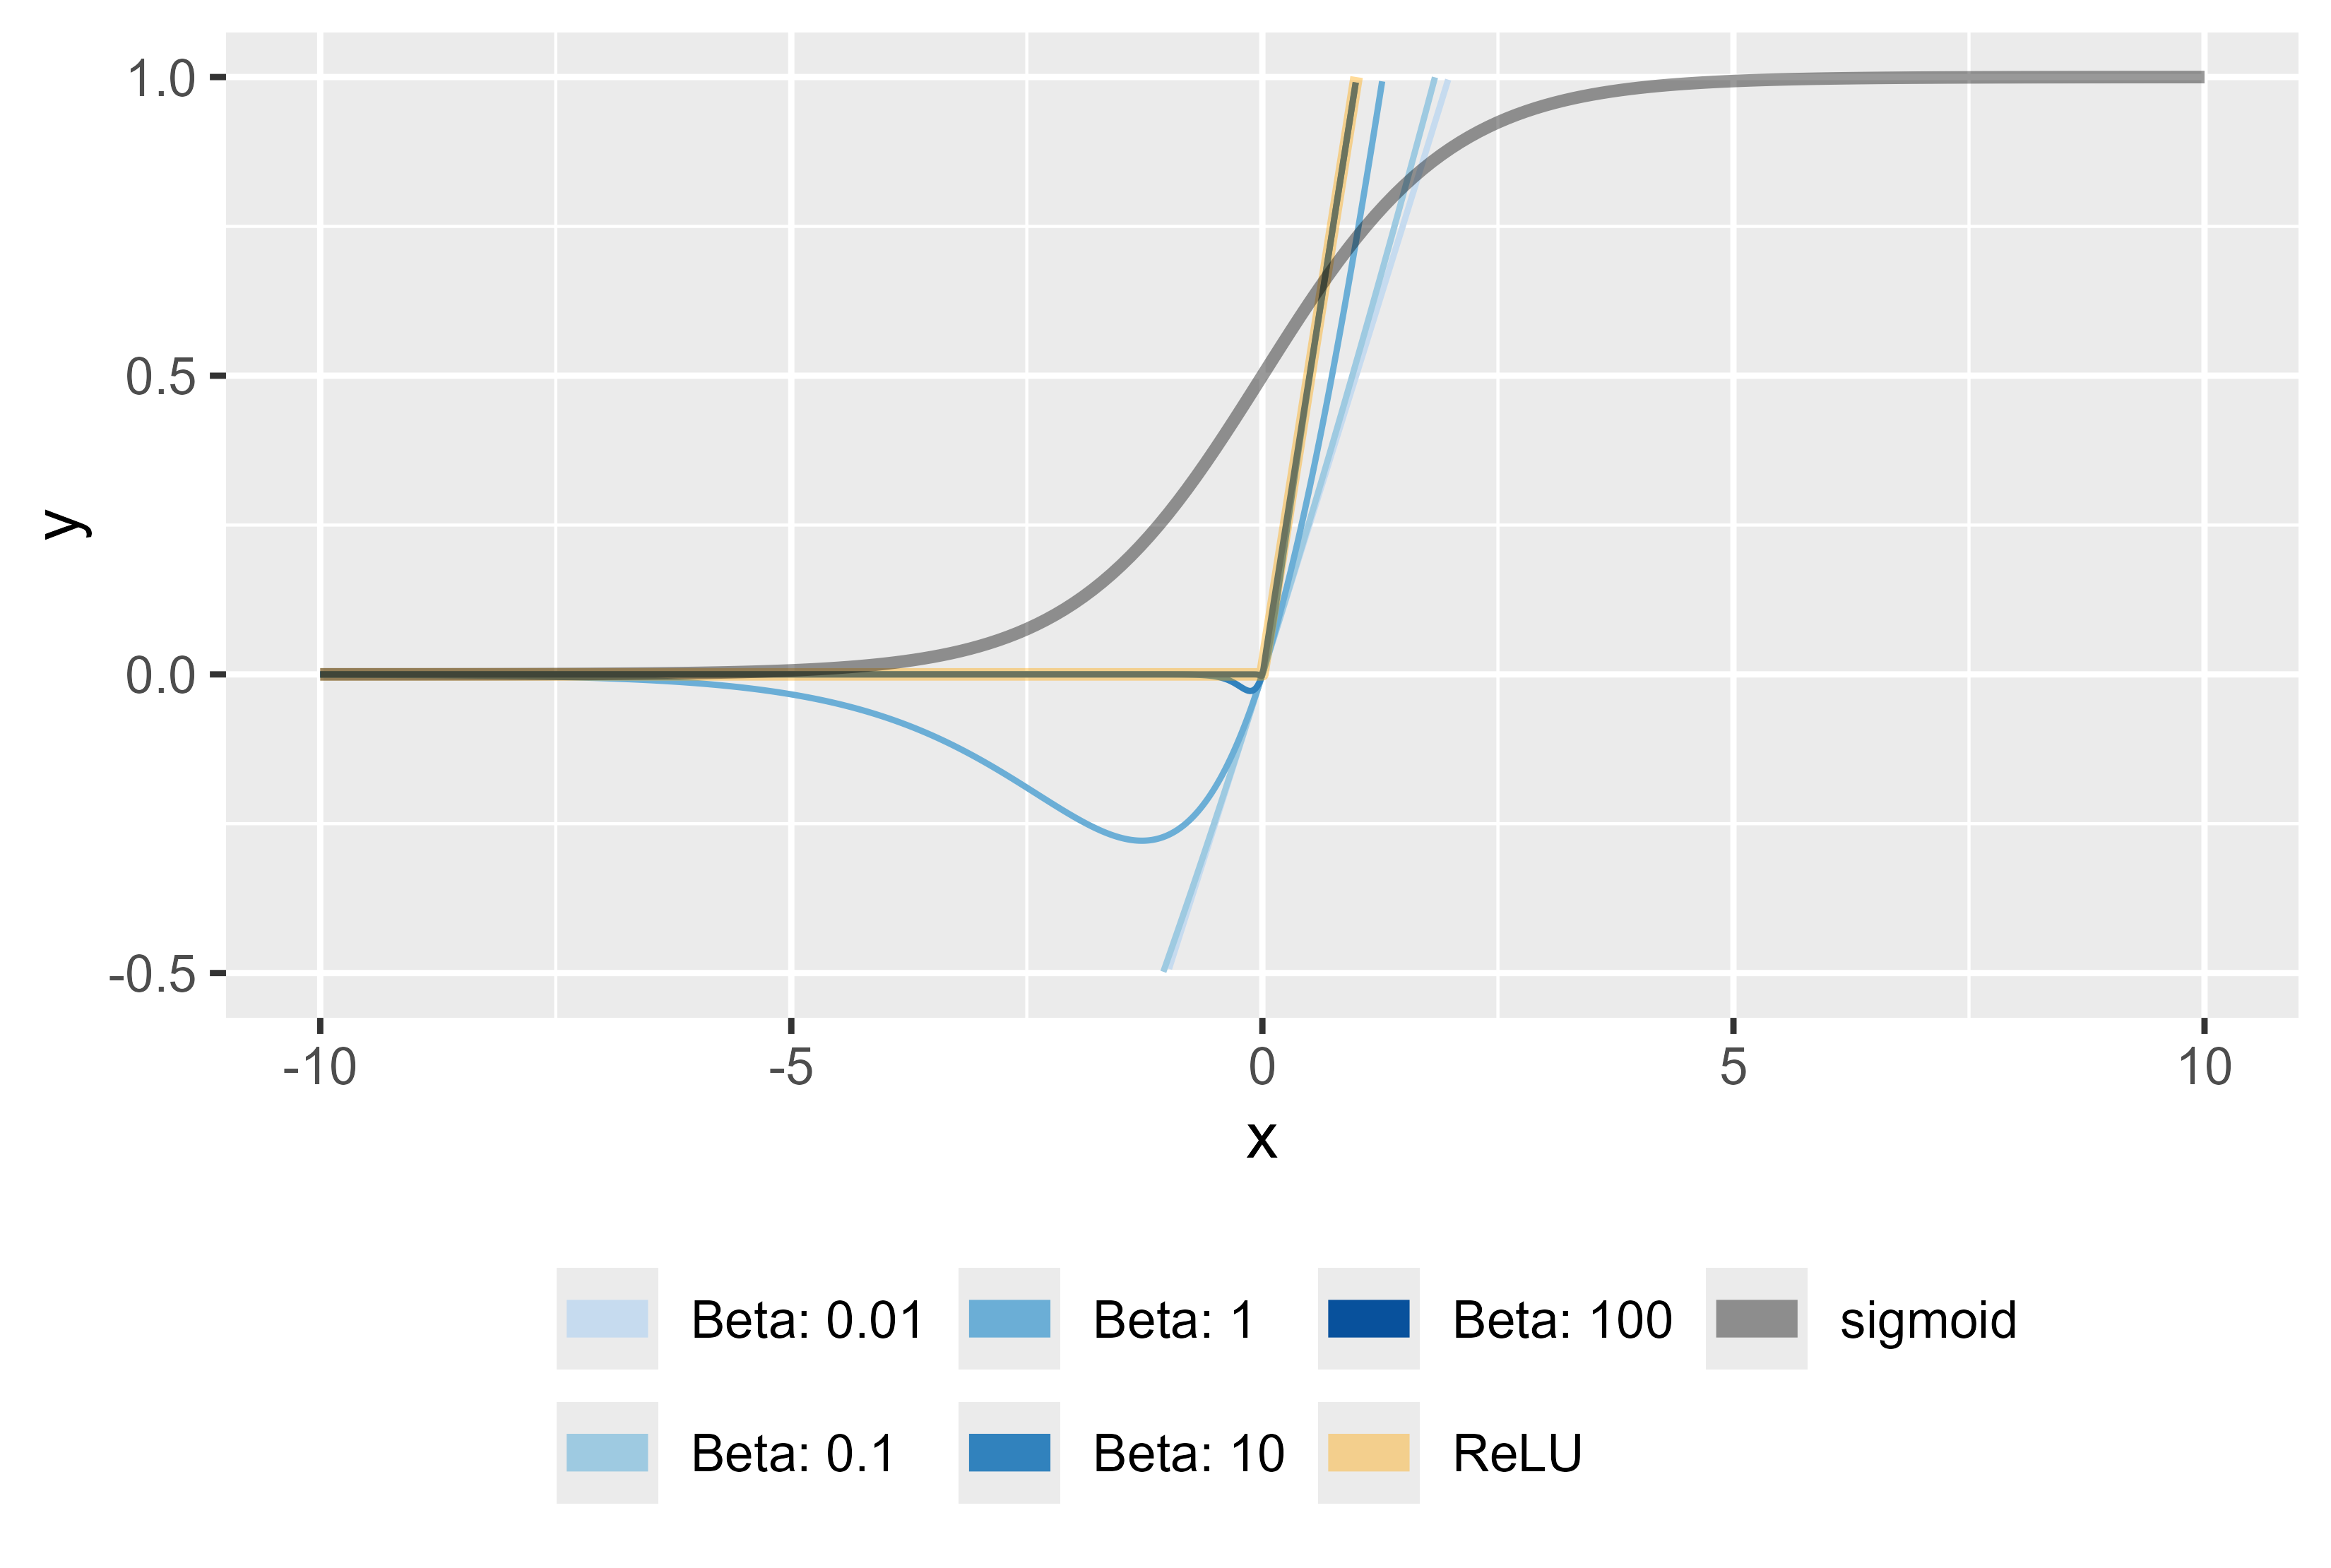
\includegraphics[width=0.8\textwidth]{plots/swish_relu_representation.png}
\caption{Swish-Funktion, ReLU Repräsentation}
\label{fig:swish_rep}
\end{figure}

Geht das \(\beta \to \infty = ReLU()\) so repräsentiert die Swish-Funktion die aktuelle ReLU-Funktion. Bei schon relativ hohem \(\beta\) erreicht die swish-Funktion approximiert die ReLU-Funktion. Geht das \(\beta \to 0 = x\), so entspricht die Funktion x.

\subsection{Auto Regressive-Moving Average (ARIMA)}\label{auto-regressive-moving-average-arima}

Bei dem (S)ARIMA Modell handelt es sich um ein additives statistisches Modell, welches sich an komplexe Zeitreihen anpasst. Dabei beschreiben die Thermen PDQ (saisonall) und pdq (nicht saisonall) das Modell. Folgende Backshift Notation beschreibt
das Modell:

\[
\Phi(B)\phi(B)(1-B)^d (1-B)^D y_t = c + \Theta(B) \theta(B) \epsilon_t
\]

Dabei wird die Zeitreihe d-mal und D-mal differenziert. Die Thermen p, d, P, Q werden mittels des geringsten AICc ermittelt. Dieses Modell gilt als eines der Grundlagenmodelle zum Vergleich in dieser Arbeit. \cite{HyndmanR}

\subsection{PROPHET: Forecasting at a scale}\label{prophet-forecasting-at-a-scale}

Das Prophet-Model wurde von Facebook \cite{taylor2018forecasting} entwickelt und findet Anwendung beim Vorhersagen von Zeitreihen mit komplexer Saisonalität.
Speziell designt, um Feiertag-Muster zu erkennen. Dabei handelt es sich wie bei dem ARIMA Modell um ein additives Modell. Im Vergleich zum ARIMA Modell ist das Prophet-Model vor allem im Training deutlich schneller. Hinzu kommt, dass dieses Modell im Gegensatz zum ARIMA Modell den Effekt der Feiertage deutlich besser erfassen kann. Folgende Formel beschreibt das Modell:

\[
y(t) = g(t) + s(t) + h(t) + \epsilon_t
\]

g(t) : Der schrittweise lineare Trend

s(t) : Die saisonalen Muster

h(t) : Feiertag-Mustererfassung

\(\epsilon_t\) : Der Fehler-Term (Rauschen)

\clearpage
\newpage

\subsection{Metriken}\label{metriken}

Als ein Auswahlkriterium für eine Vorhersage spielen Metriken wie Mean Absolute Error (MAE), Mean Absolute Percentage Error (MAPE) und Root Mean Squared Error (RMSE) eine Rolle. Folgend werden die einzelnen Metriken kurz beschrieben.

\textbf{MAE} beschreibt die durchschnittliche absolute Abweichung zwischen den vorhergesagten Werten \(\hat{y_i}\) und den tatsächlichen Werten \(y_i\). Folgende Formel wird dabei verwendet:

\[
MAE = \sum_{i=1}^{n} \frac{| y_i - \hat{y_i} | }{n}
\]

\textbf{MAPE} beschreibt die durchschnittliche prozentuale Abweichung zwischen den vorhergesagten Werten \(\hat{y_i}\) und den tatsächlichen Werten \(y_i\). Folgende Formel wird dabei verwendet.

\[
MAPE = 100 \frac{1}{n} \sum_{i=1}^{n} | \frac{ y_i - \hat{y_i}  }{y_i} |
\]

\textbf{RMSE} beschreibt die Durchschnittliche quadratische Abweichung zwischen den vorhergesagten Werten \(\hat{y_i}\) und den tatsächlichen Werten \(y_i\). Folgende Formel wird dabei verwendet.

\[
RMSE = \sqrt{\frac{1}{n} \sum_{i=1}^{n}  (y_i - \hat{y_i})^2}
\]

\clearpage
\newpage

\section{Datengrundlage und Datenanalyse}\label{datengrundlage-und-datenanalyse}

Auch für neuronale Netze muss Datenanalyse betrieben werden. Es ist wichtig, den Datensatz komplett zu durchdringen und die Erkenntnisse aus der Analyse in der Implementierung des neuronalen Netzes mitzuberücksichtigen. Der rohe Datensatz der Stromerzeugung hat eine stündliche Granularität in der Zeitspanne 01.10.2004 - 03.08.2018 (5054 Tage). Wird der Datensatz auf Äquidistanz, so fallen insgesamt 40 fehlende Beobachtungen in der stündlichen Auflösung. Die Abbildung \ref{fig:raw_AEP} repräsentiert den rohen Datensatz. Die fehlenden Werte (rot) wurden mit dem letzten vorhandenen Wert ersetzt. Dies ist damit zu begründen, da der Datensatz groß genug ist und es keine drastischen Auswirkungen auf das neuronale Netz haben wird. Nach der Säuberung der Daten hat der Datensatz korrekterweise 121.296 (\(24*5054\)) Beobachtungen. Ein positiver oder negativer Trend ist für die Stromerzeugung nicht zu erkennen.

\begin{figure}[H]
\centering
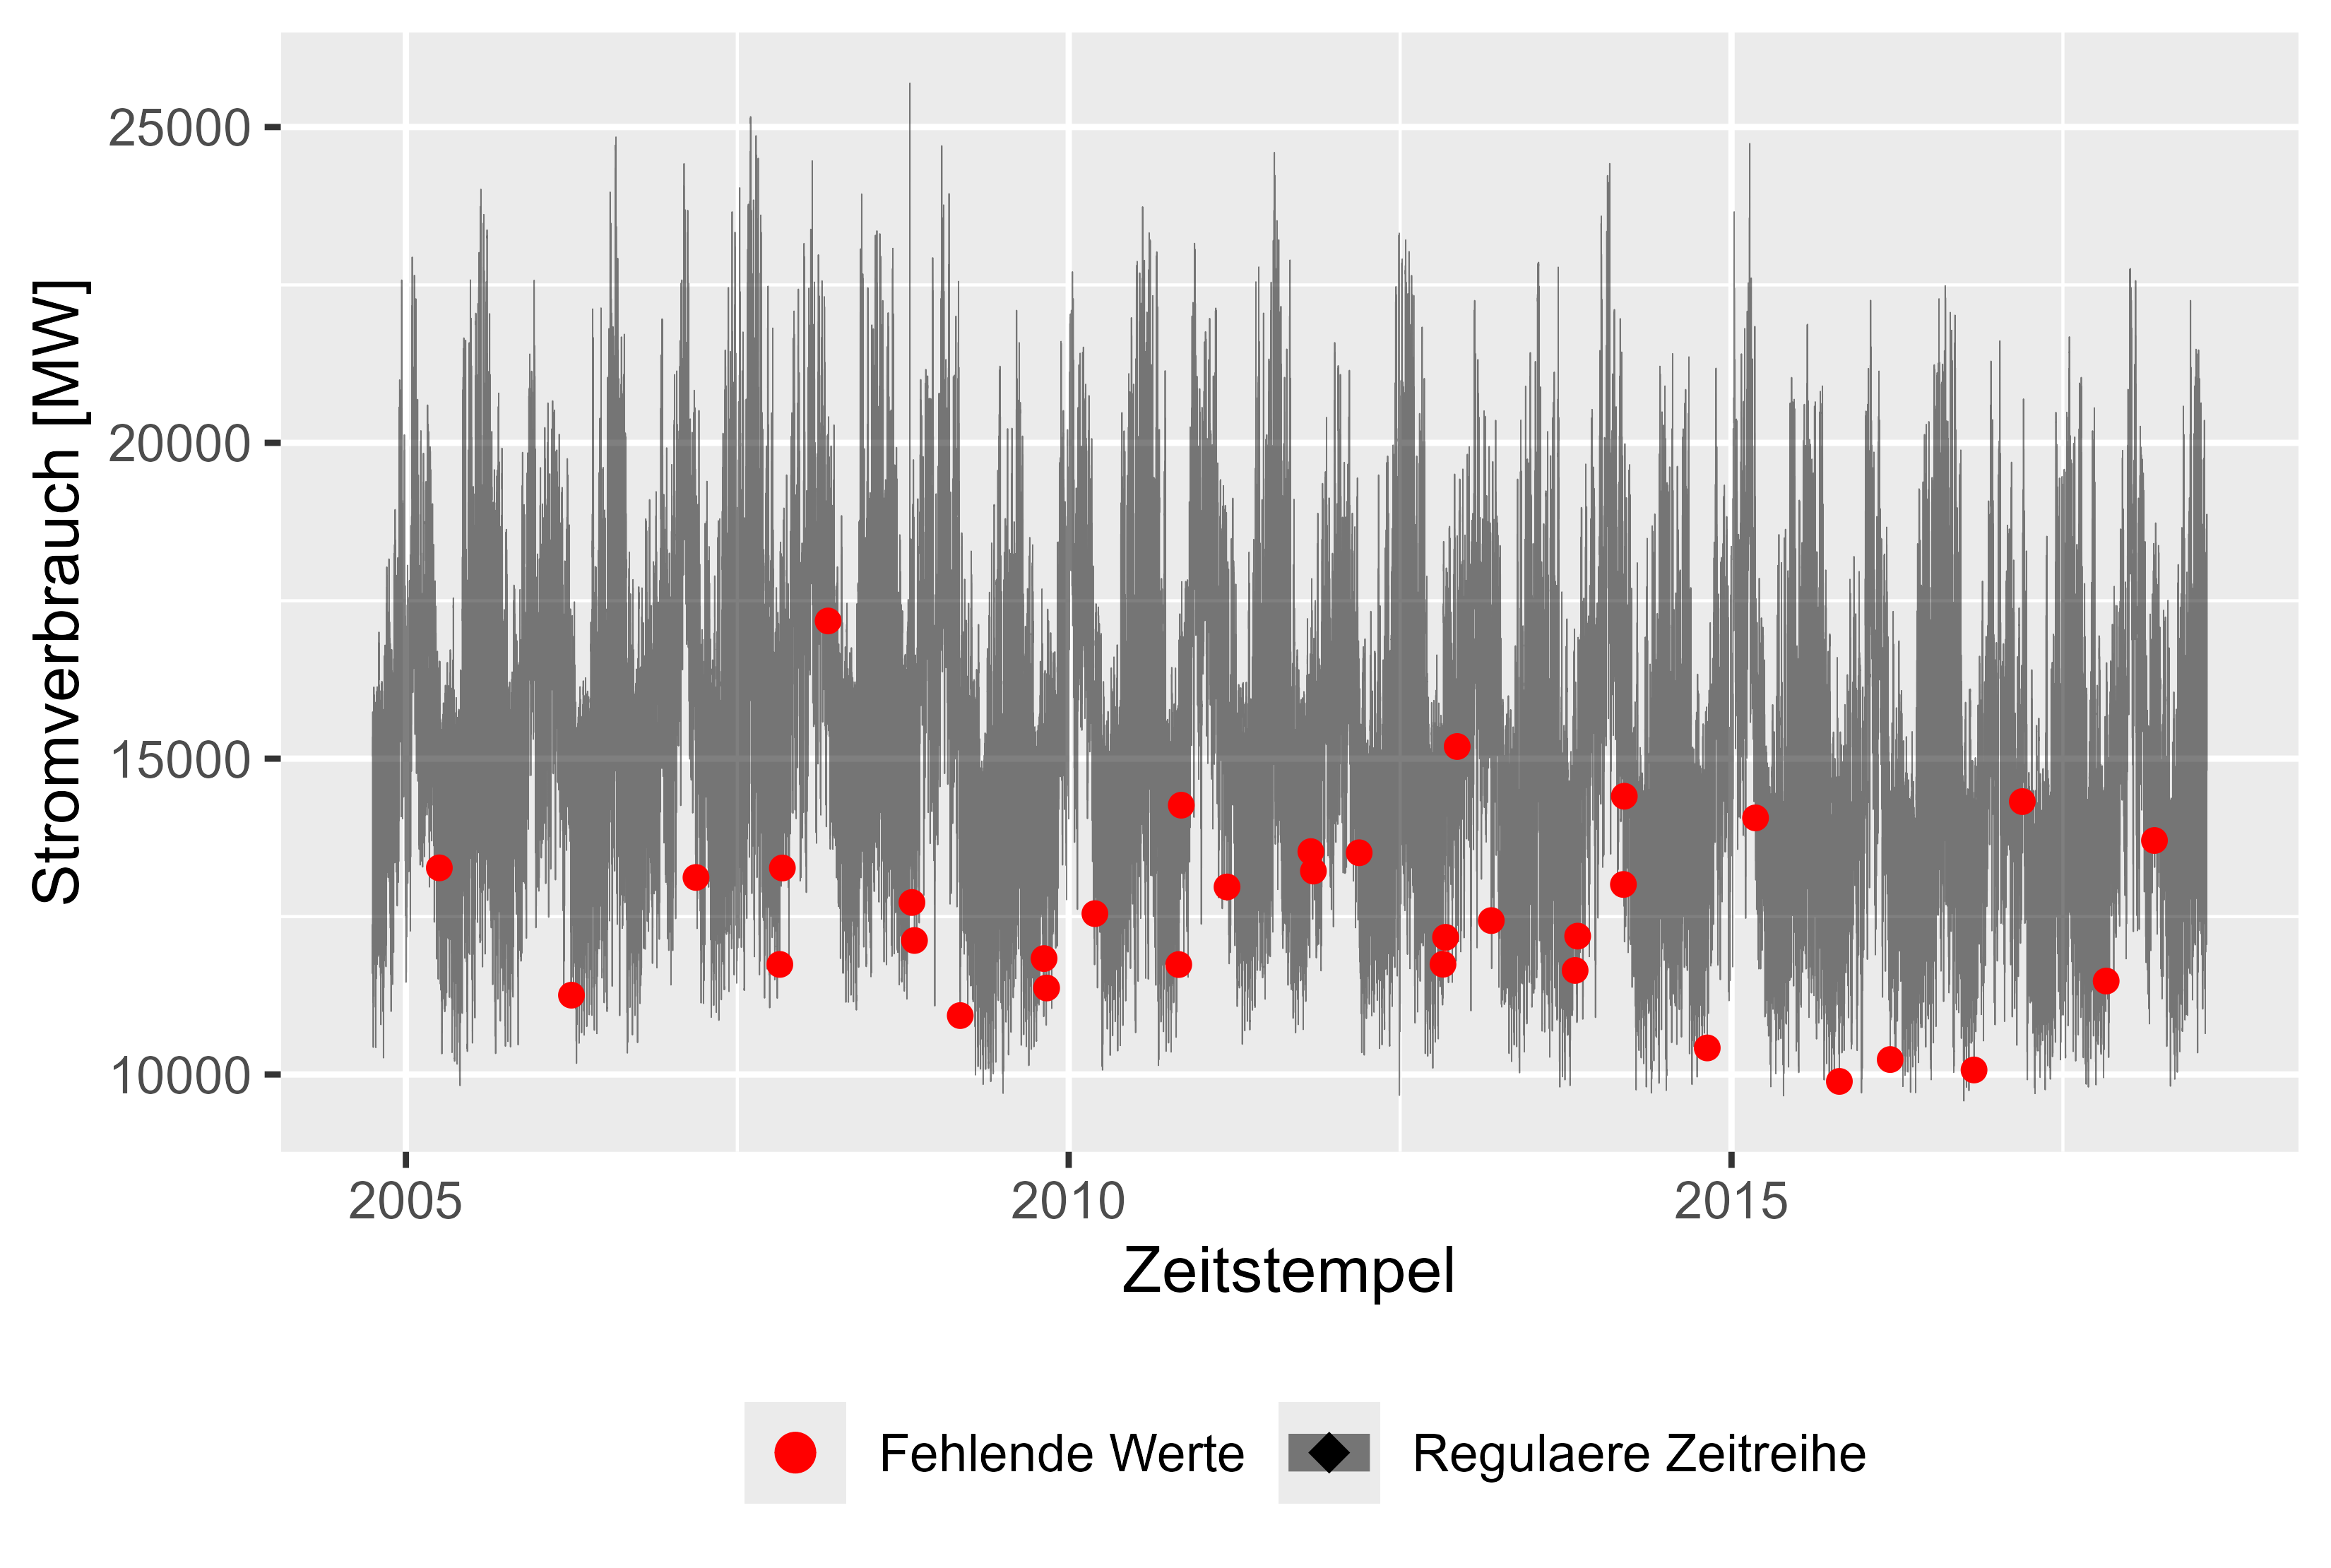
\includegraphics[width=1.0\textwidth]{plots/raw_AEP_MW.png}
\caption{Roher Datensatz zur Stromerzeugung (01.10.2004 - 03.08.2018) vom Unternehmen American Electric Power}
\label{fig:raw_AEP}
\end{figure}

Wird der Datensatz der Stromerzeugung in die einzelnen Jahre aufgespalten, so ist deutlich ein moustache-Muster (Schnurrbart) zu erkennen. Dieses Muster kann in der Abbildung \ref{fig:raw_years} entnommen werden.

\begin{figure}[H]
\centering
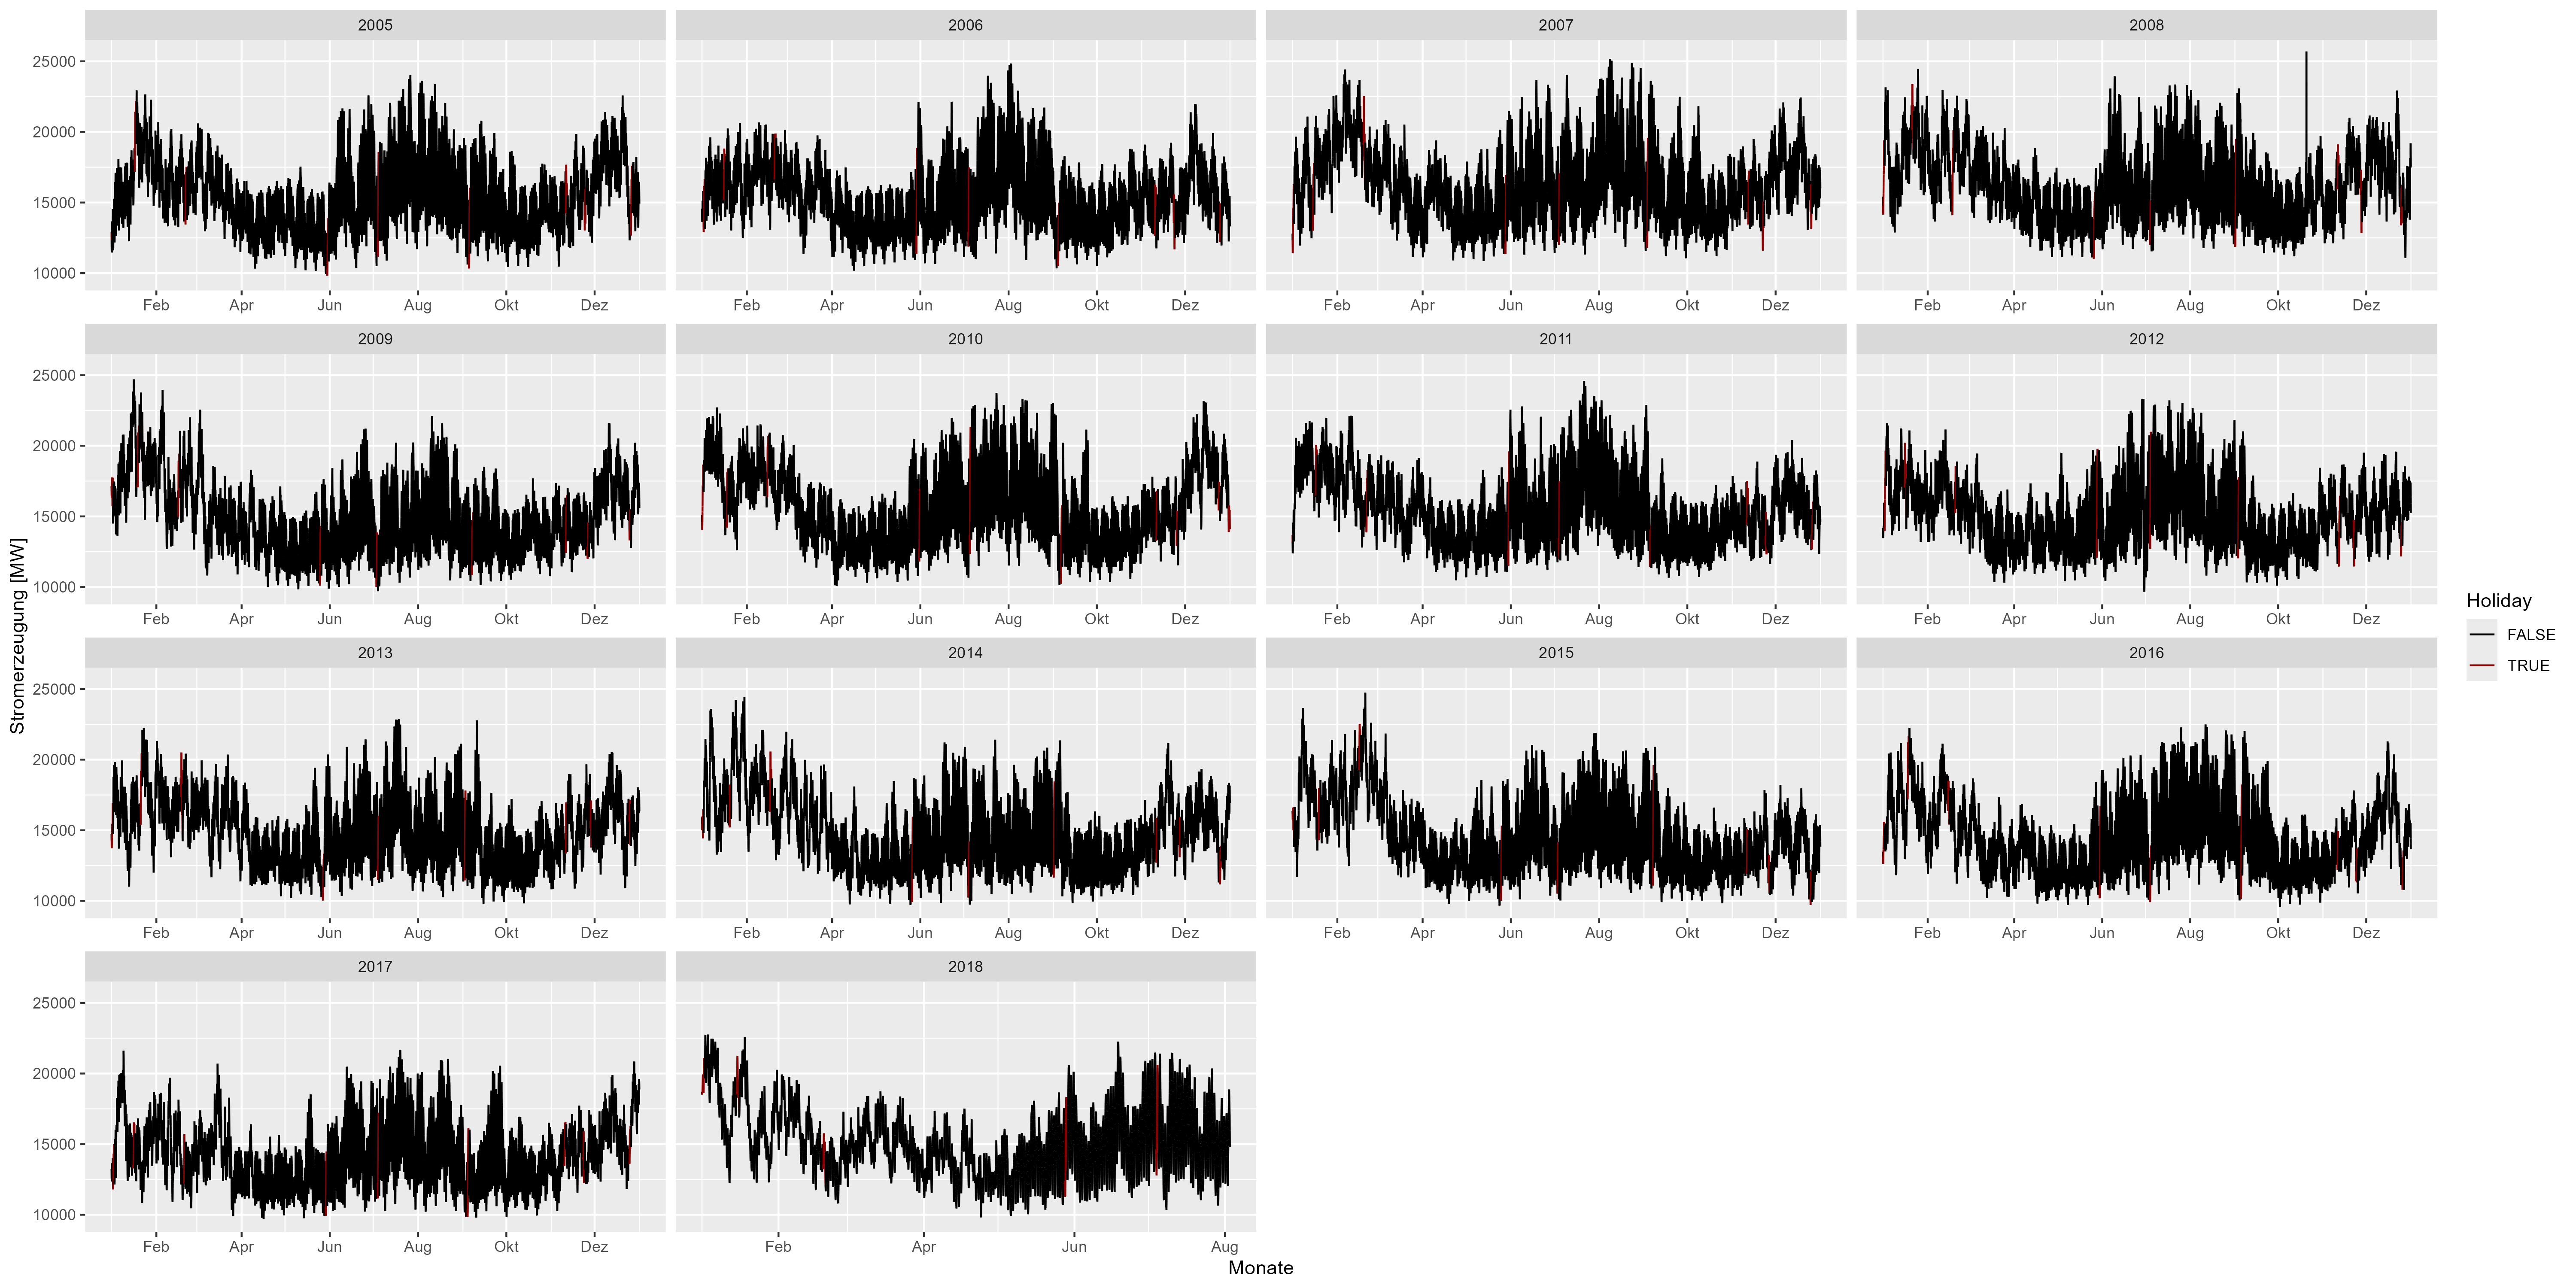
\includegraphics[width=1.0\textwidth]{plots/raw_years.png}
\caption{Stromerzeugung aufgespalten in einzelne Jahre}
\label{fig:raw_years}
\end{figure}

Auch die Verteilung der Daten kann eine Rolle bei der Modellierung der neuronalen Netze spielen. Die Stromerzeugung besitzt einen minimalen Wert von 9581 MW, einen maximalen Wert von 25.695MW und einen Durchschnitt von 15.499 MW. Die Abbildung \ref{fig:histogram} zeigt die Verteilung der Stromerzeugung (normalverteilt).

\begin{figure}[H]
\centering
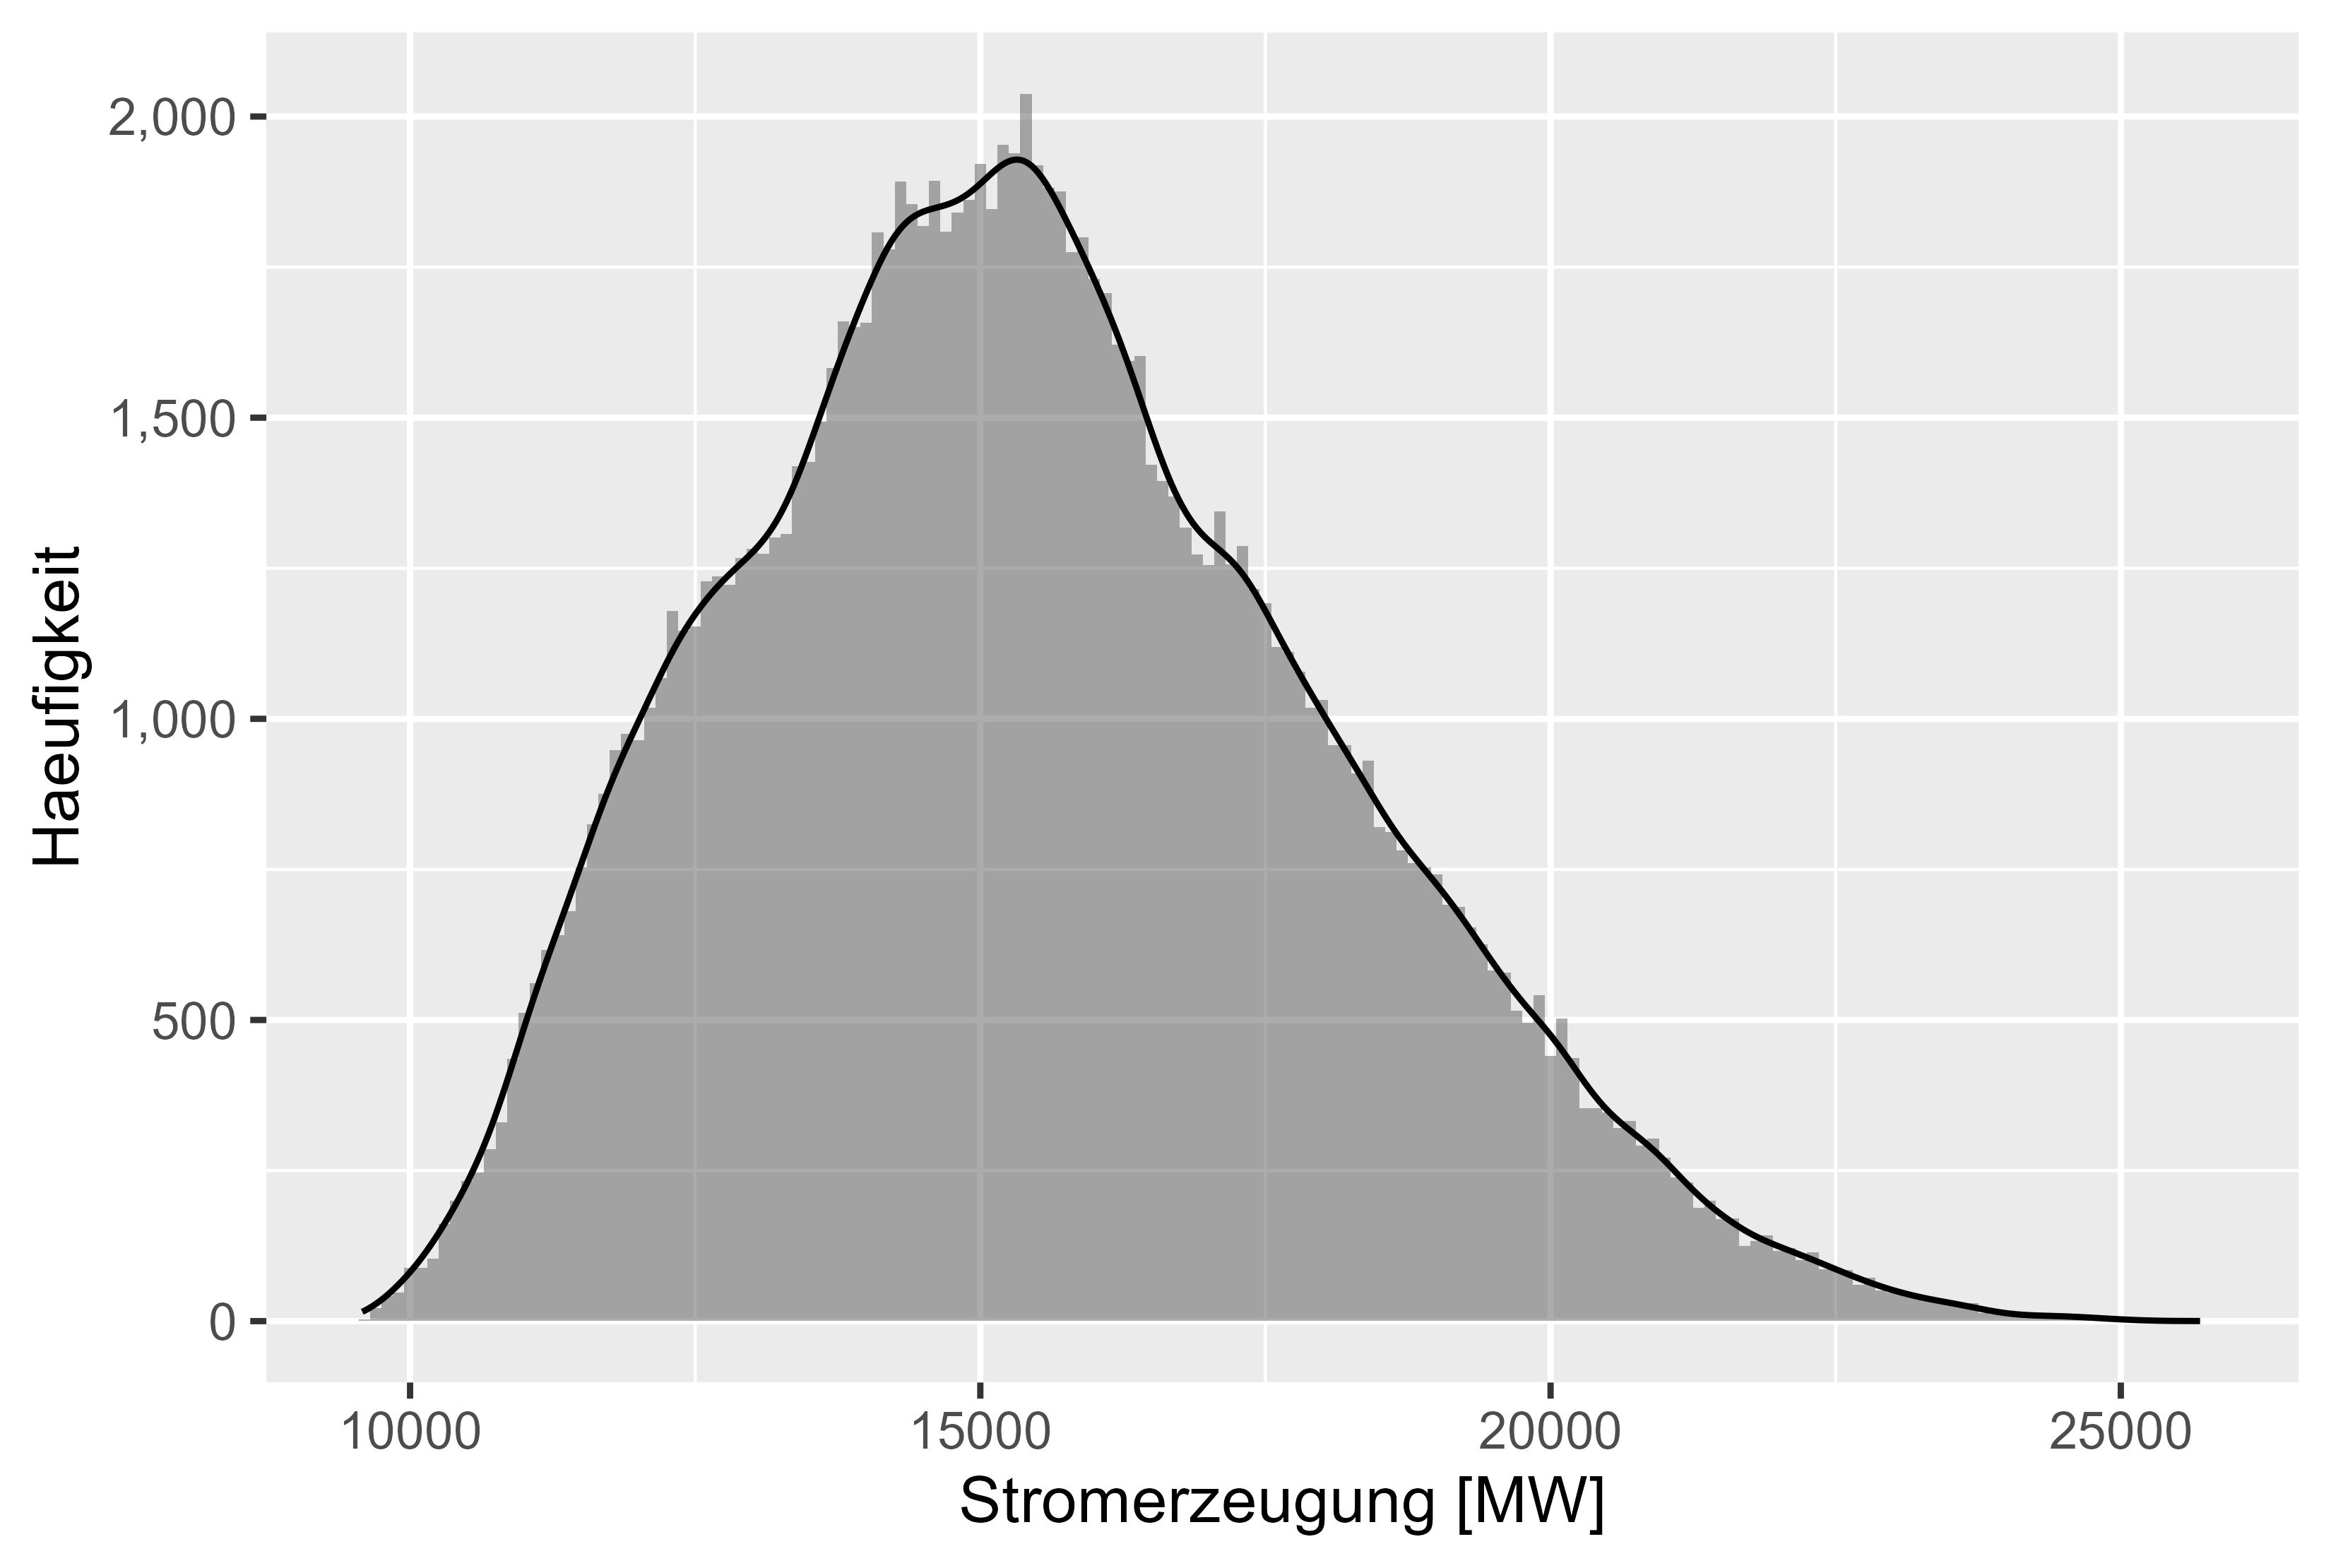
\includegraphics[width=1.0\textwidth]{plots/histogram.png}
\caption{Verteilung der Stromerzeugung}
\label{fig:histogram}
\end{figure}

Wird der Datensatz pro Stunde aggregiert, so ist auch ein weiteres Muster innerhalb der einzelnen Tage zu erkennen. So wird die Stromerzeugung in der Nacht (\textasciitilde23:00 - 08:00) heruntergefahren und in der Tageszeit (\textasciitilde08:00 - 23:00) hochgefahren. Die Abbildung \ref{fig:hour_boxplot} stellt dabei die aggregierte Darstellung für jede Stunde dar.

\begin{figure}[H]
\centering
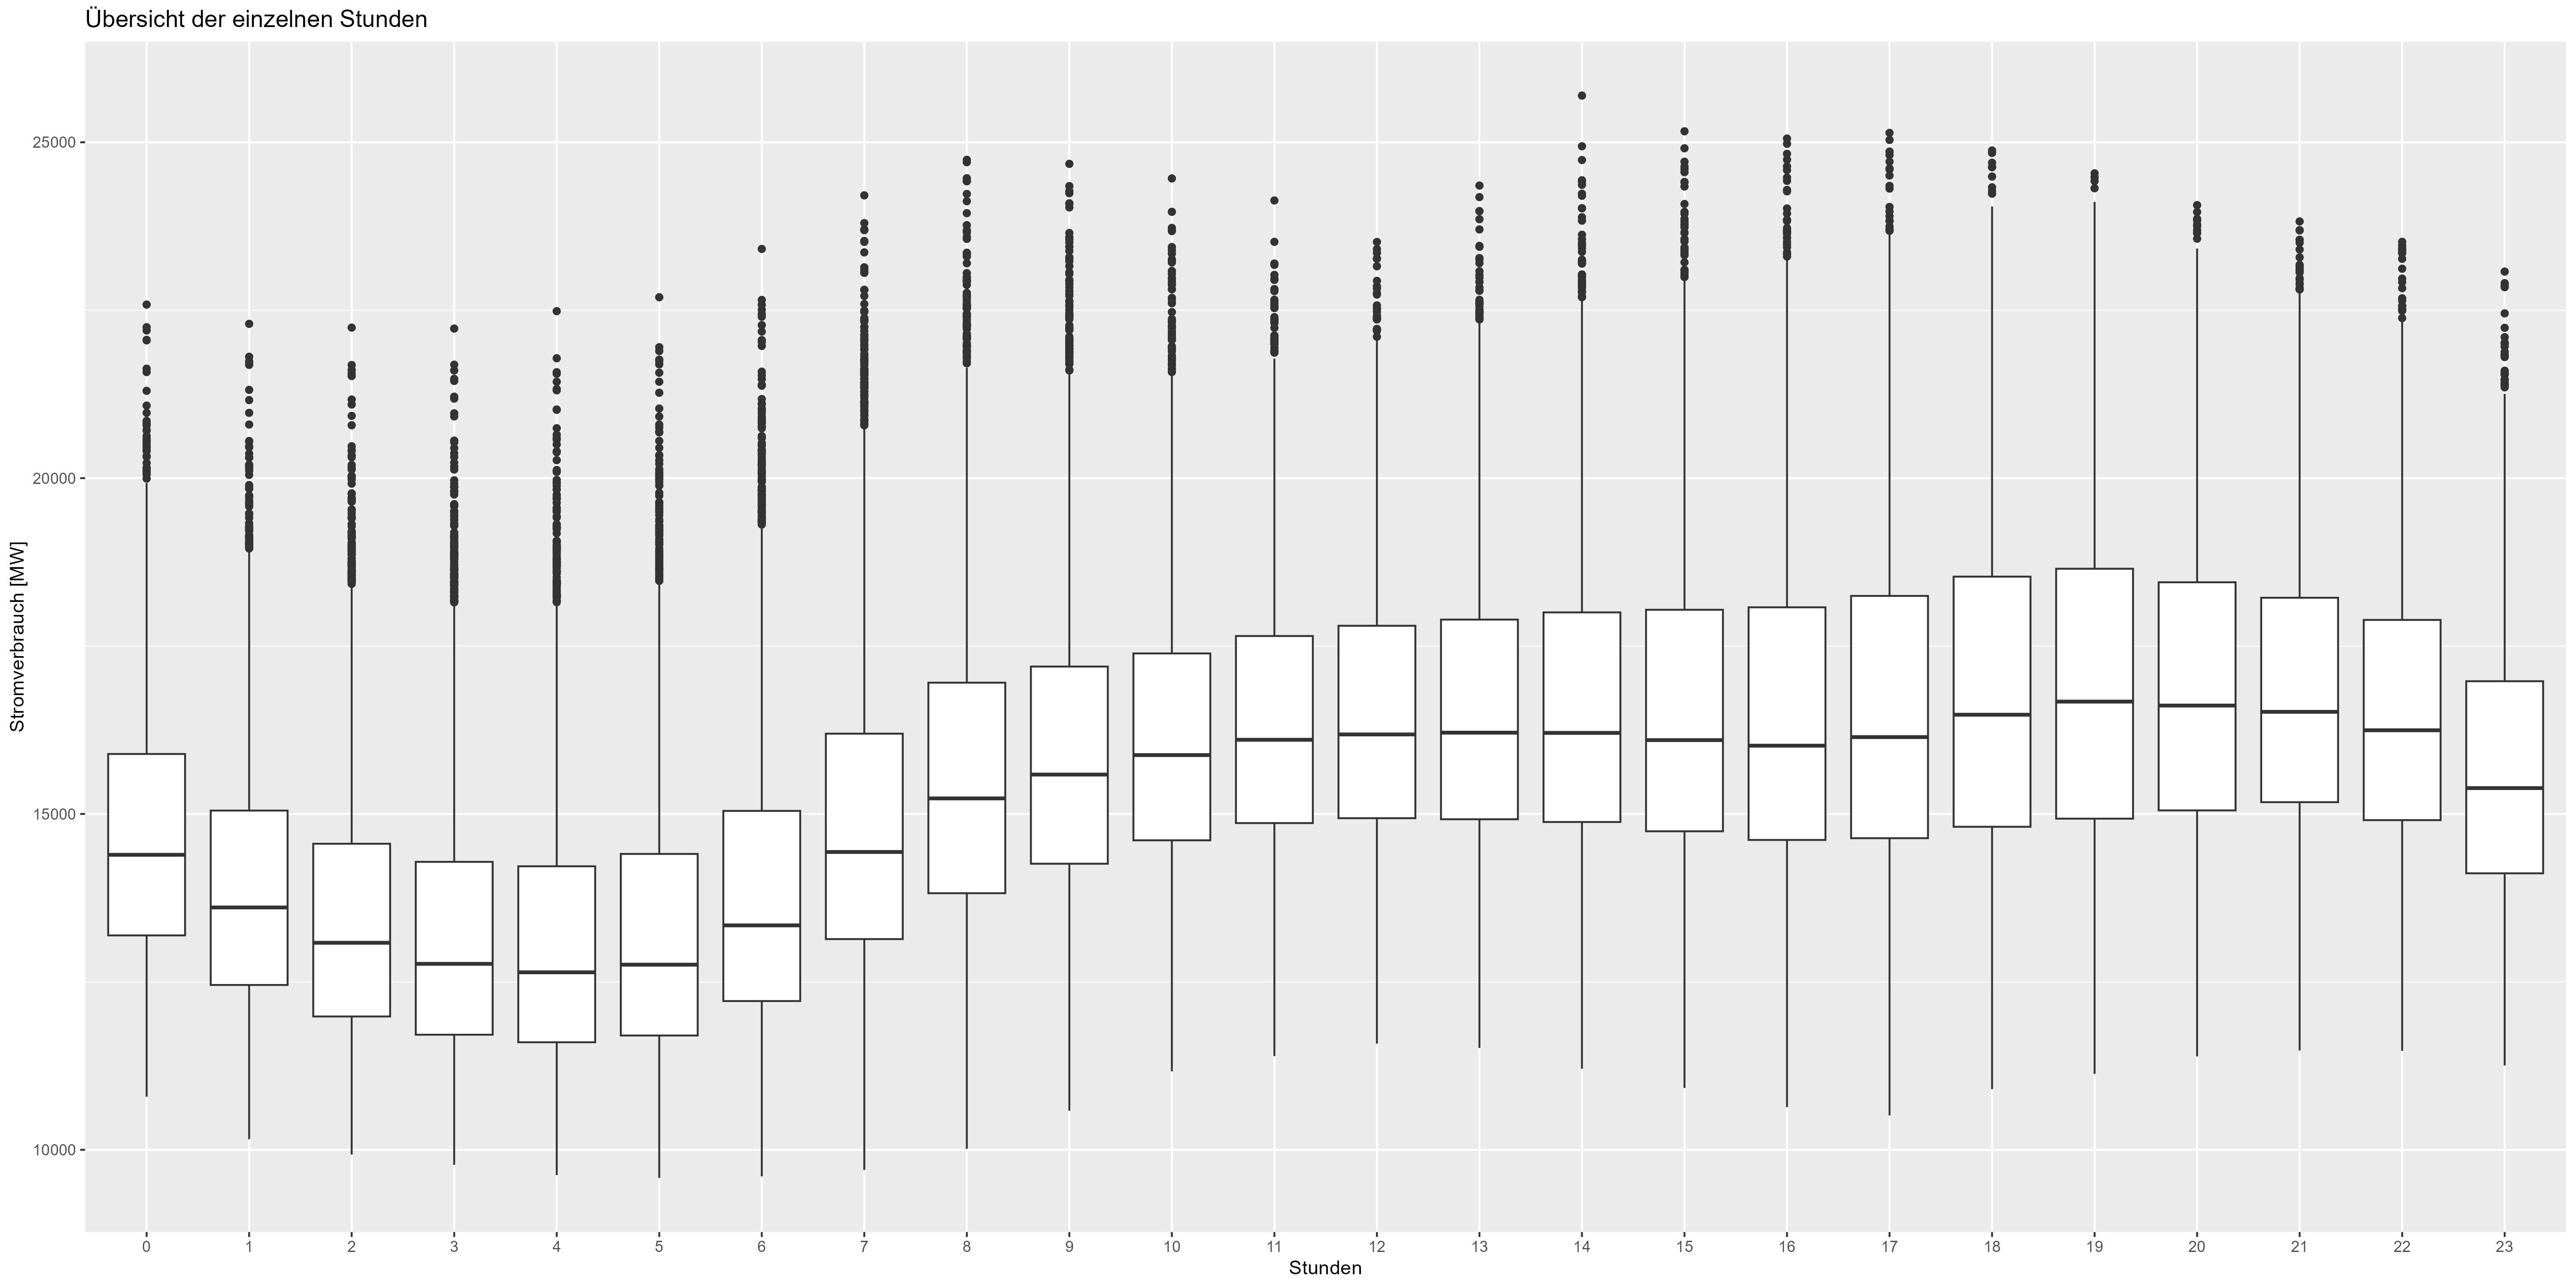
\includegraphics[width=1.0\textwidth]{plots/hour_boxplot.png}
\caption{Stündlich aggregierte Darstellung der Stromerzeugung}
\label{fig:hour_boxplot}
\end{figure}

Für ein tieferes Verständnis ist es sinnvoll, die Wochentage, Werktage und die Feiertage zu betrachten. Als Erstes die wöchentliche Betrachtung der Stromerzeugung. Die Abbildung \ref{fig:weekday_boxplot} stellt dabei die einzelnen Wochentage über die Jahre dar. Anzumerken ist, dass der Samstag und der Sonntag sich von den regulären Wochentagen in der Stromerzeugung unterscheiden. So haben die beiden Tage im Durchschnitt ca. 2000 MW weniger an Stromerzeugung.

\begin{figure}[H]
\centering
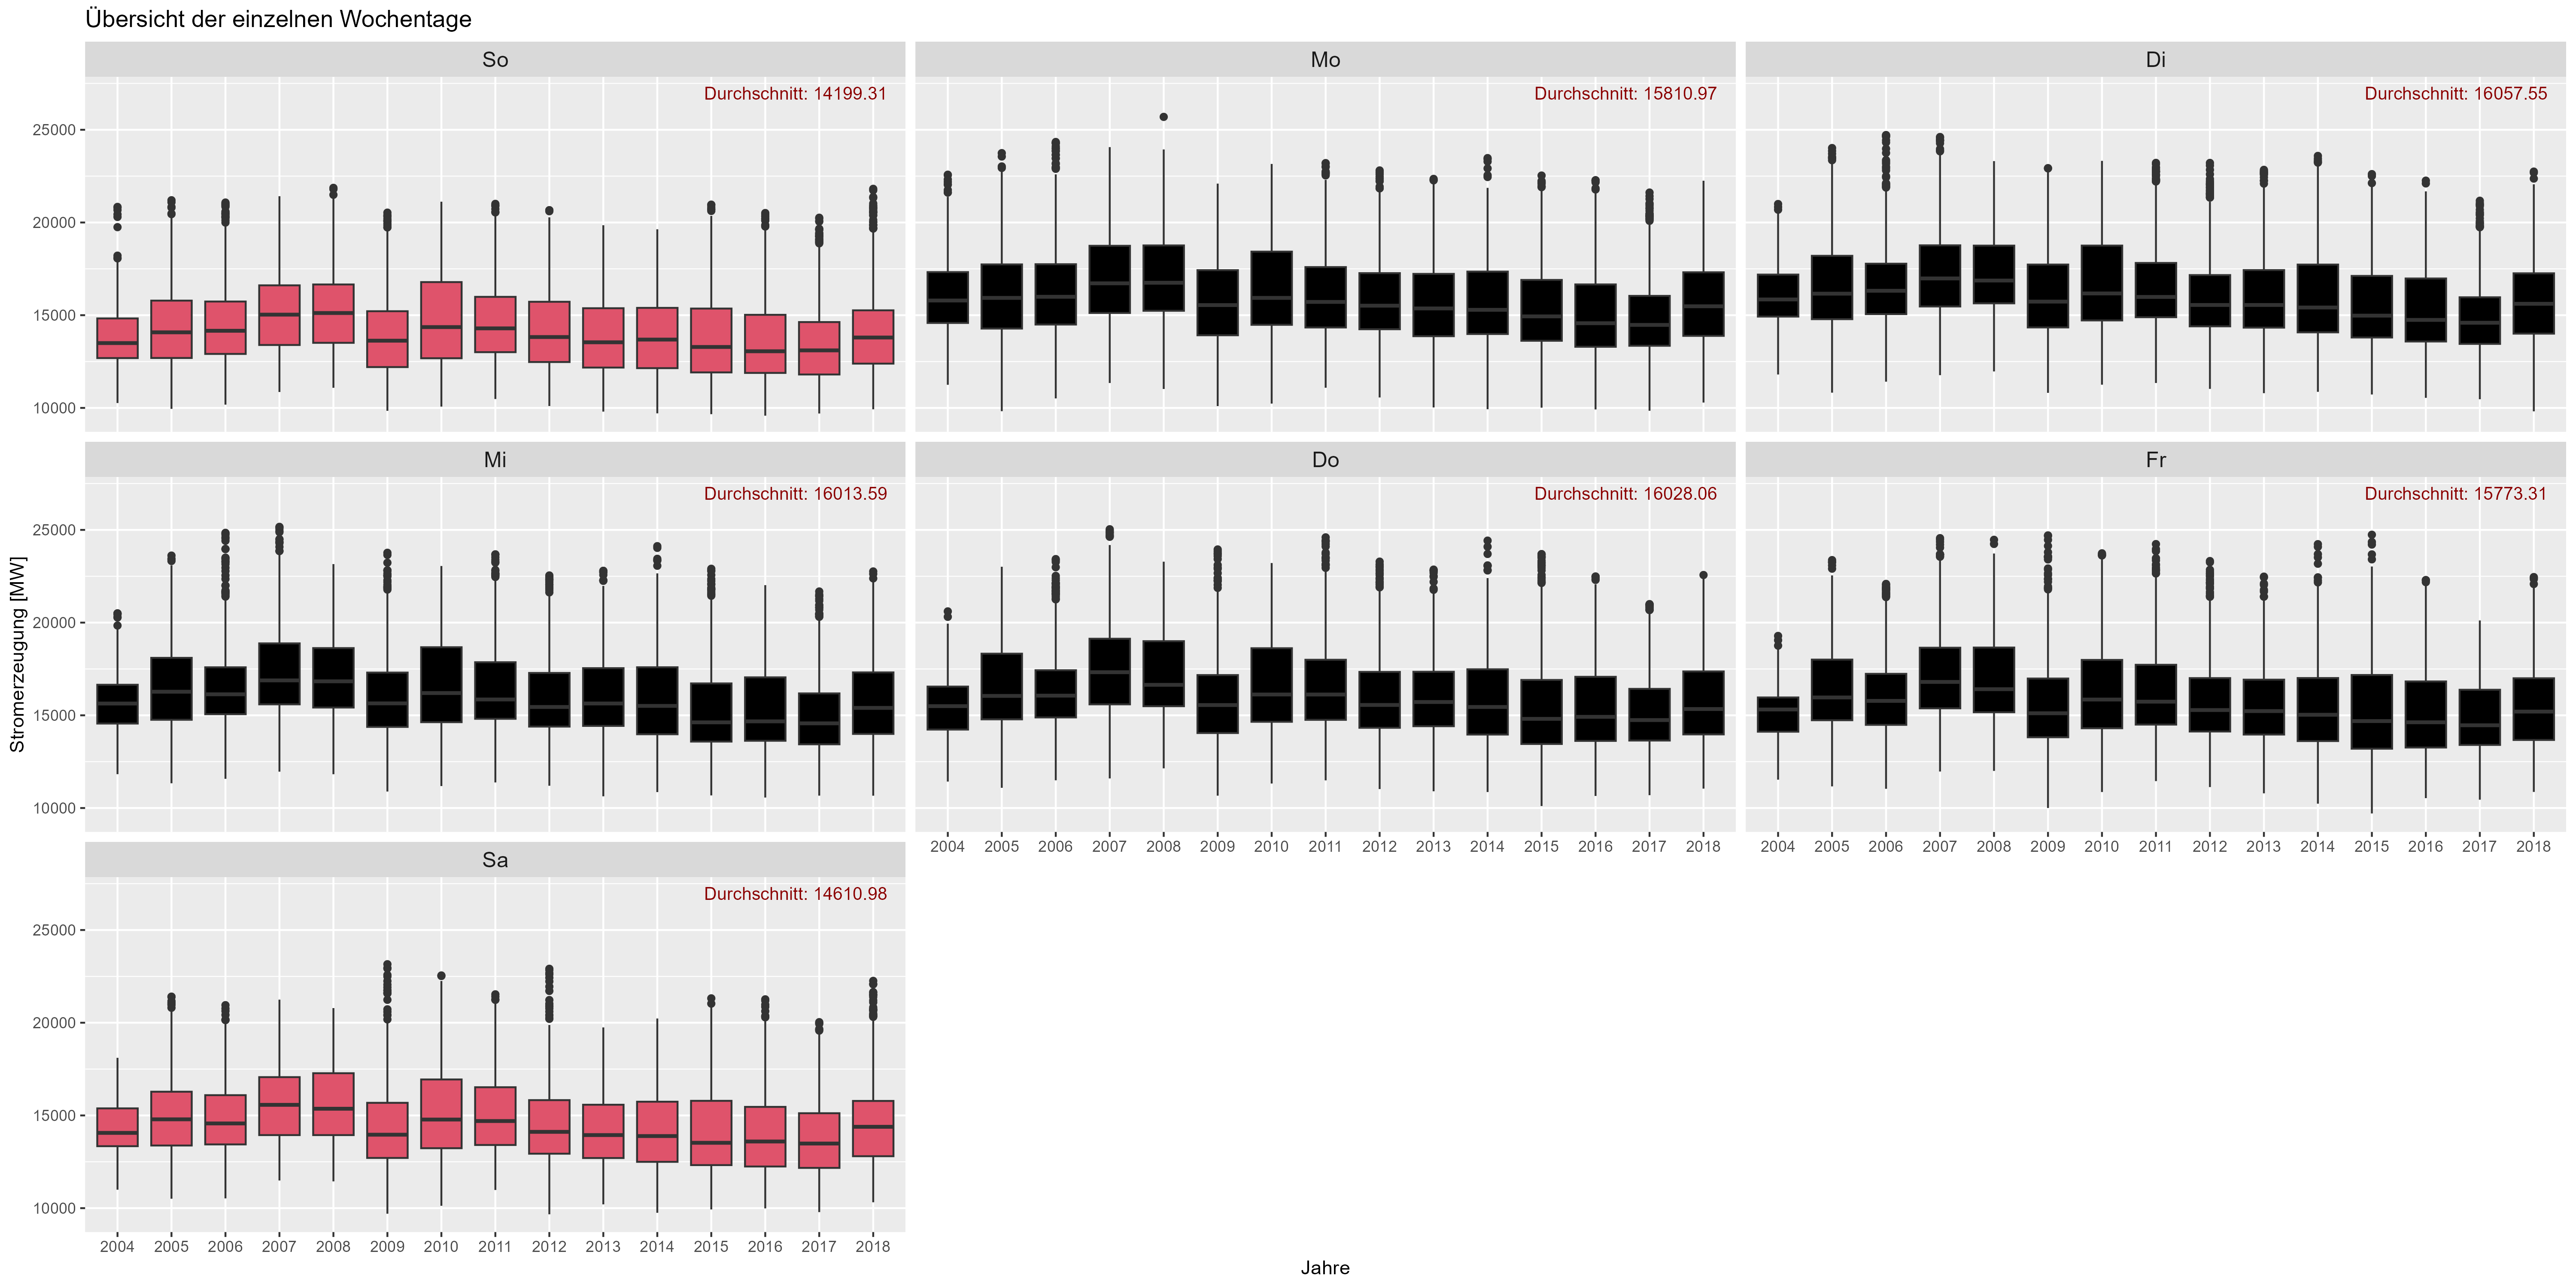
\includegraphics[width=1.0\textwidth]{plots/weekday_boxplot.png}
\caption{Wöchentlich aggregierte Darstellung der Stromerzeugung}
\label{fig:weekday_boxplot}
\end{figure}

Auch die einzelnen Feiertage unterscheiden sich von einem regulären Tag. In der Abbildung \ref{fig:holiday_boxplot} sind die einzelnen Feiertage abgebildet. Ähnliche wie ein Wochenende sinkt an den meisten Feiertagen die Stromerzeugung. Bis auf den Martin Luther Kind, Jr.~Day, New Year's Day, Veterans Day und den Washington's Birthday verhalten sich die Feiertage wie ein Wochenende unter der Betrachtung vom Durchschnitt.

\begin{figure}[H]
\centering
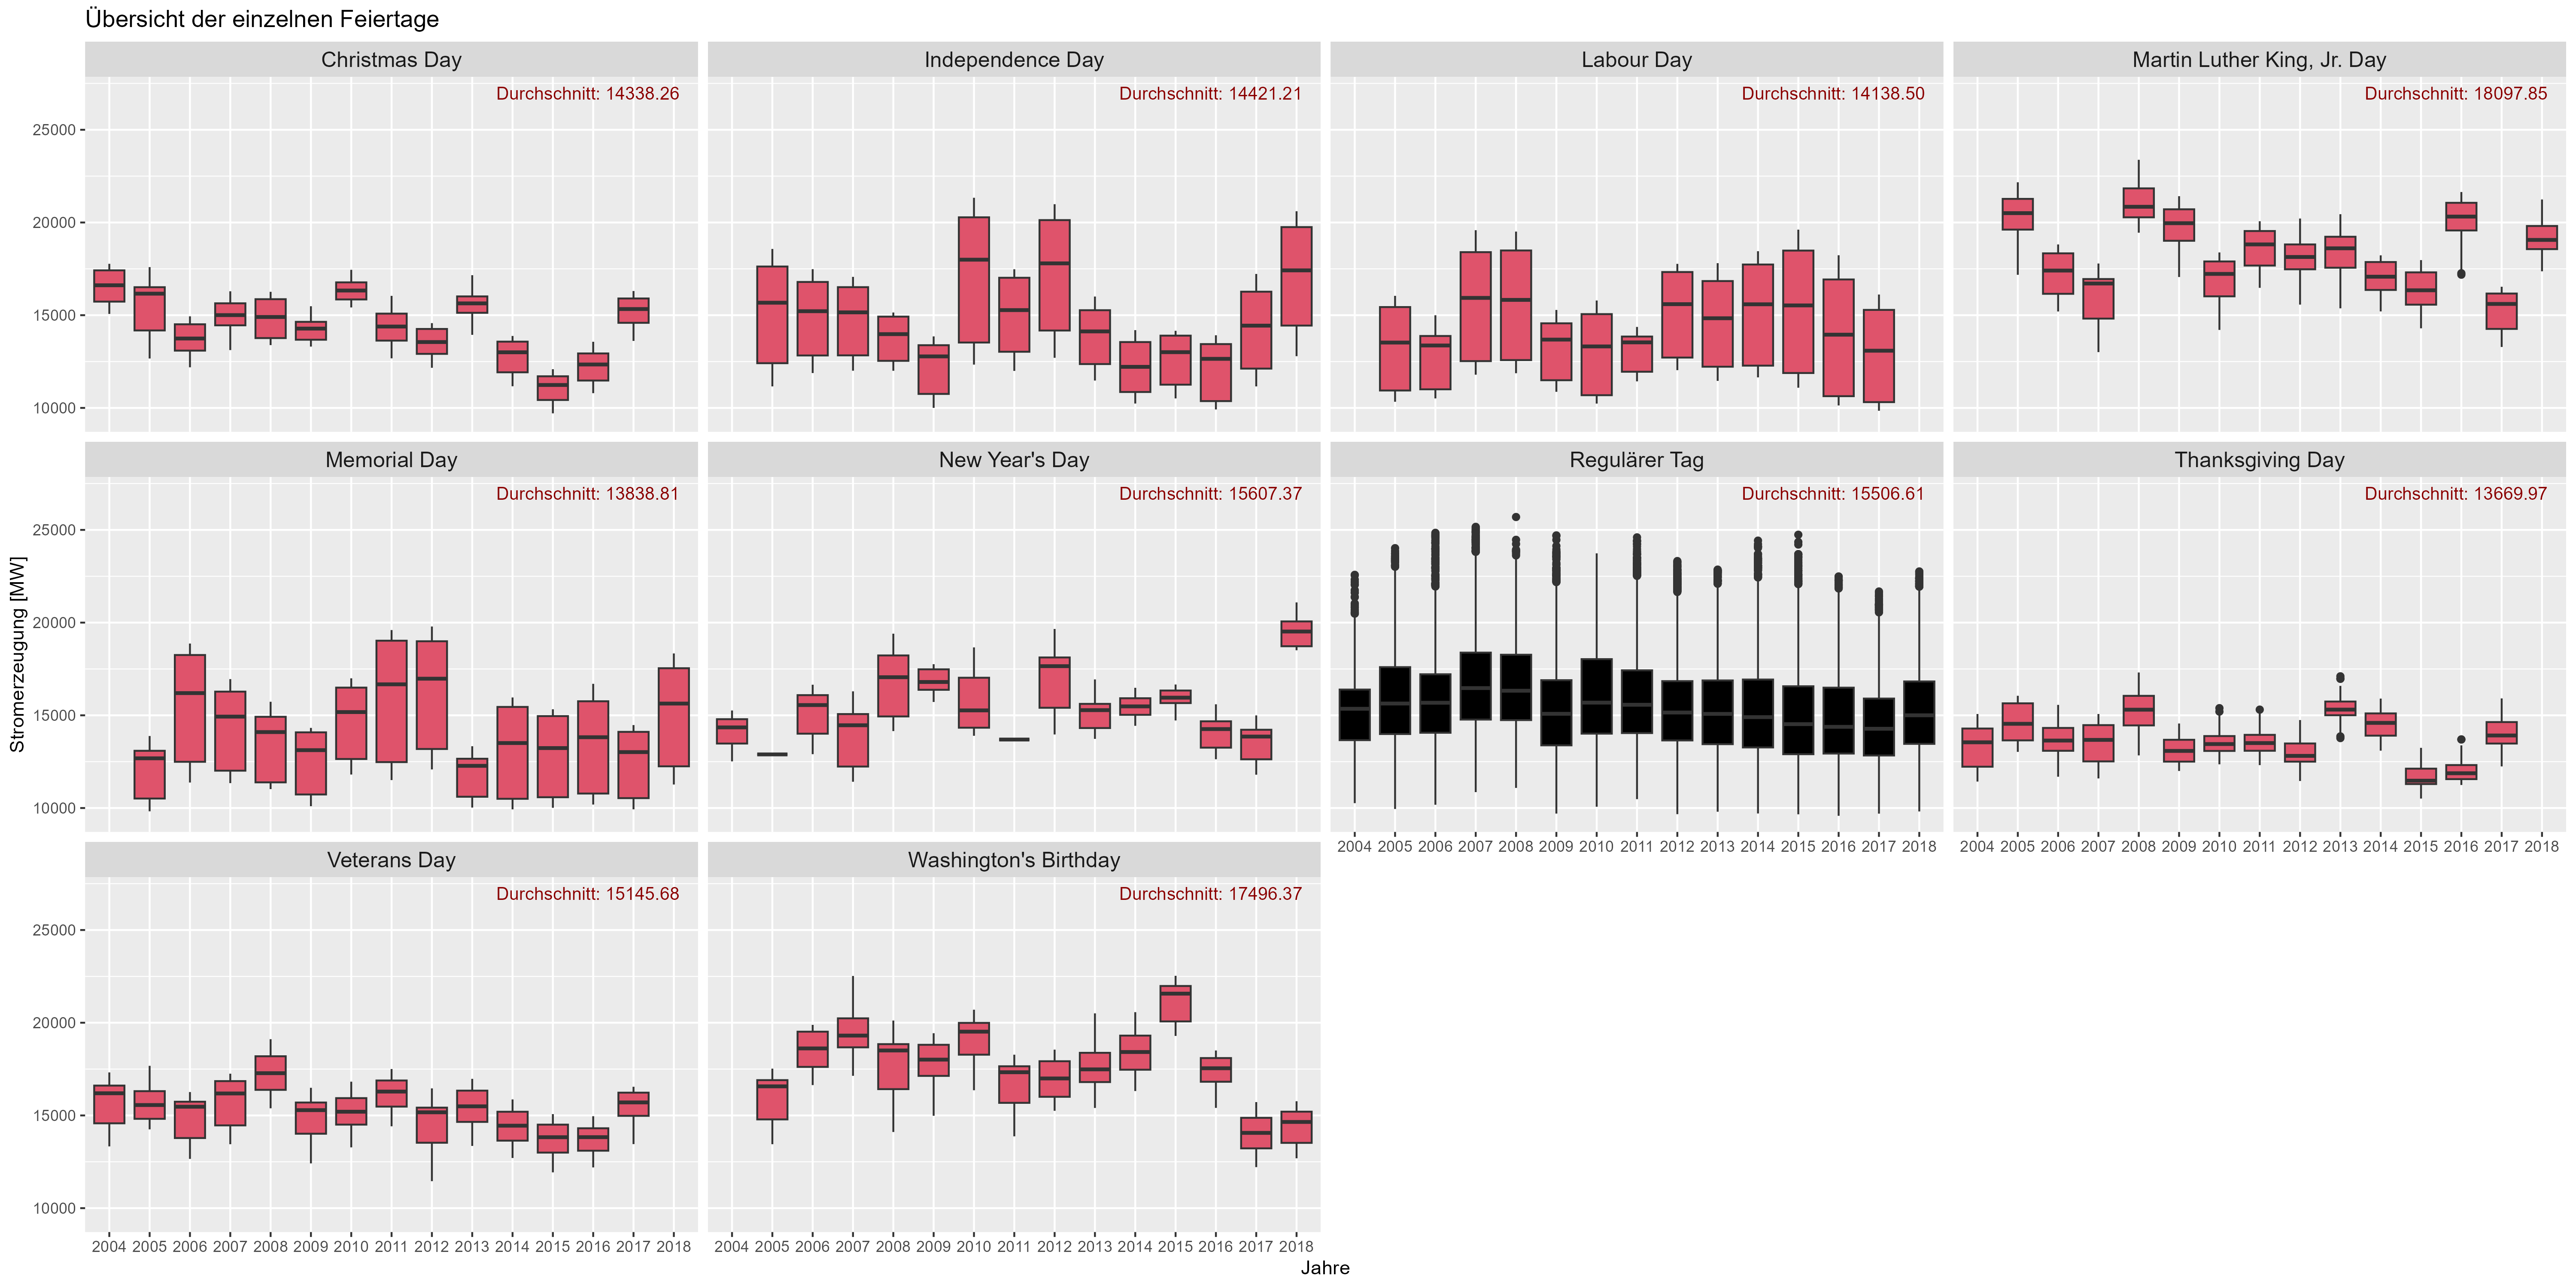
\includegraphics[width=1.0\textwidth]{plots/holiday_boxplot}
\caption{Feiertage, aggregierte Darstellung der Stromerzeugung}
\label{fig:holiday_boxplot}
\end{figure}

So kann eine dummy variable erzeugt werden, die die Feiertage, aber auch die Wochenenden beinhaltet. Die Abbildung \ref{fig:workday_histogram} stellt dabei die Verteilung der Werktage und der nicht Werktage dar. Eine Verschiebung für die nicht Werktage in eine geringere Stromerzeugung ist deutlich sichtbar.

\begin{figure}[H]
\centering
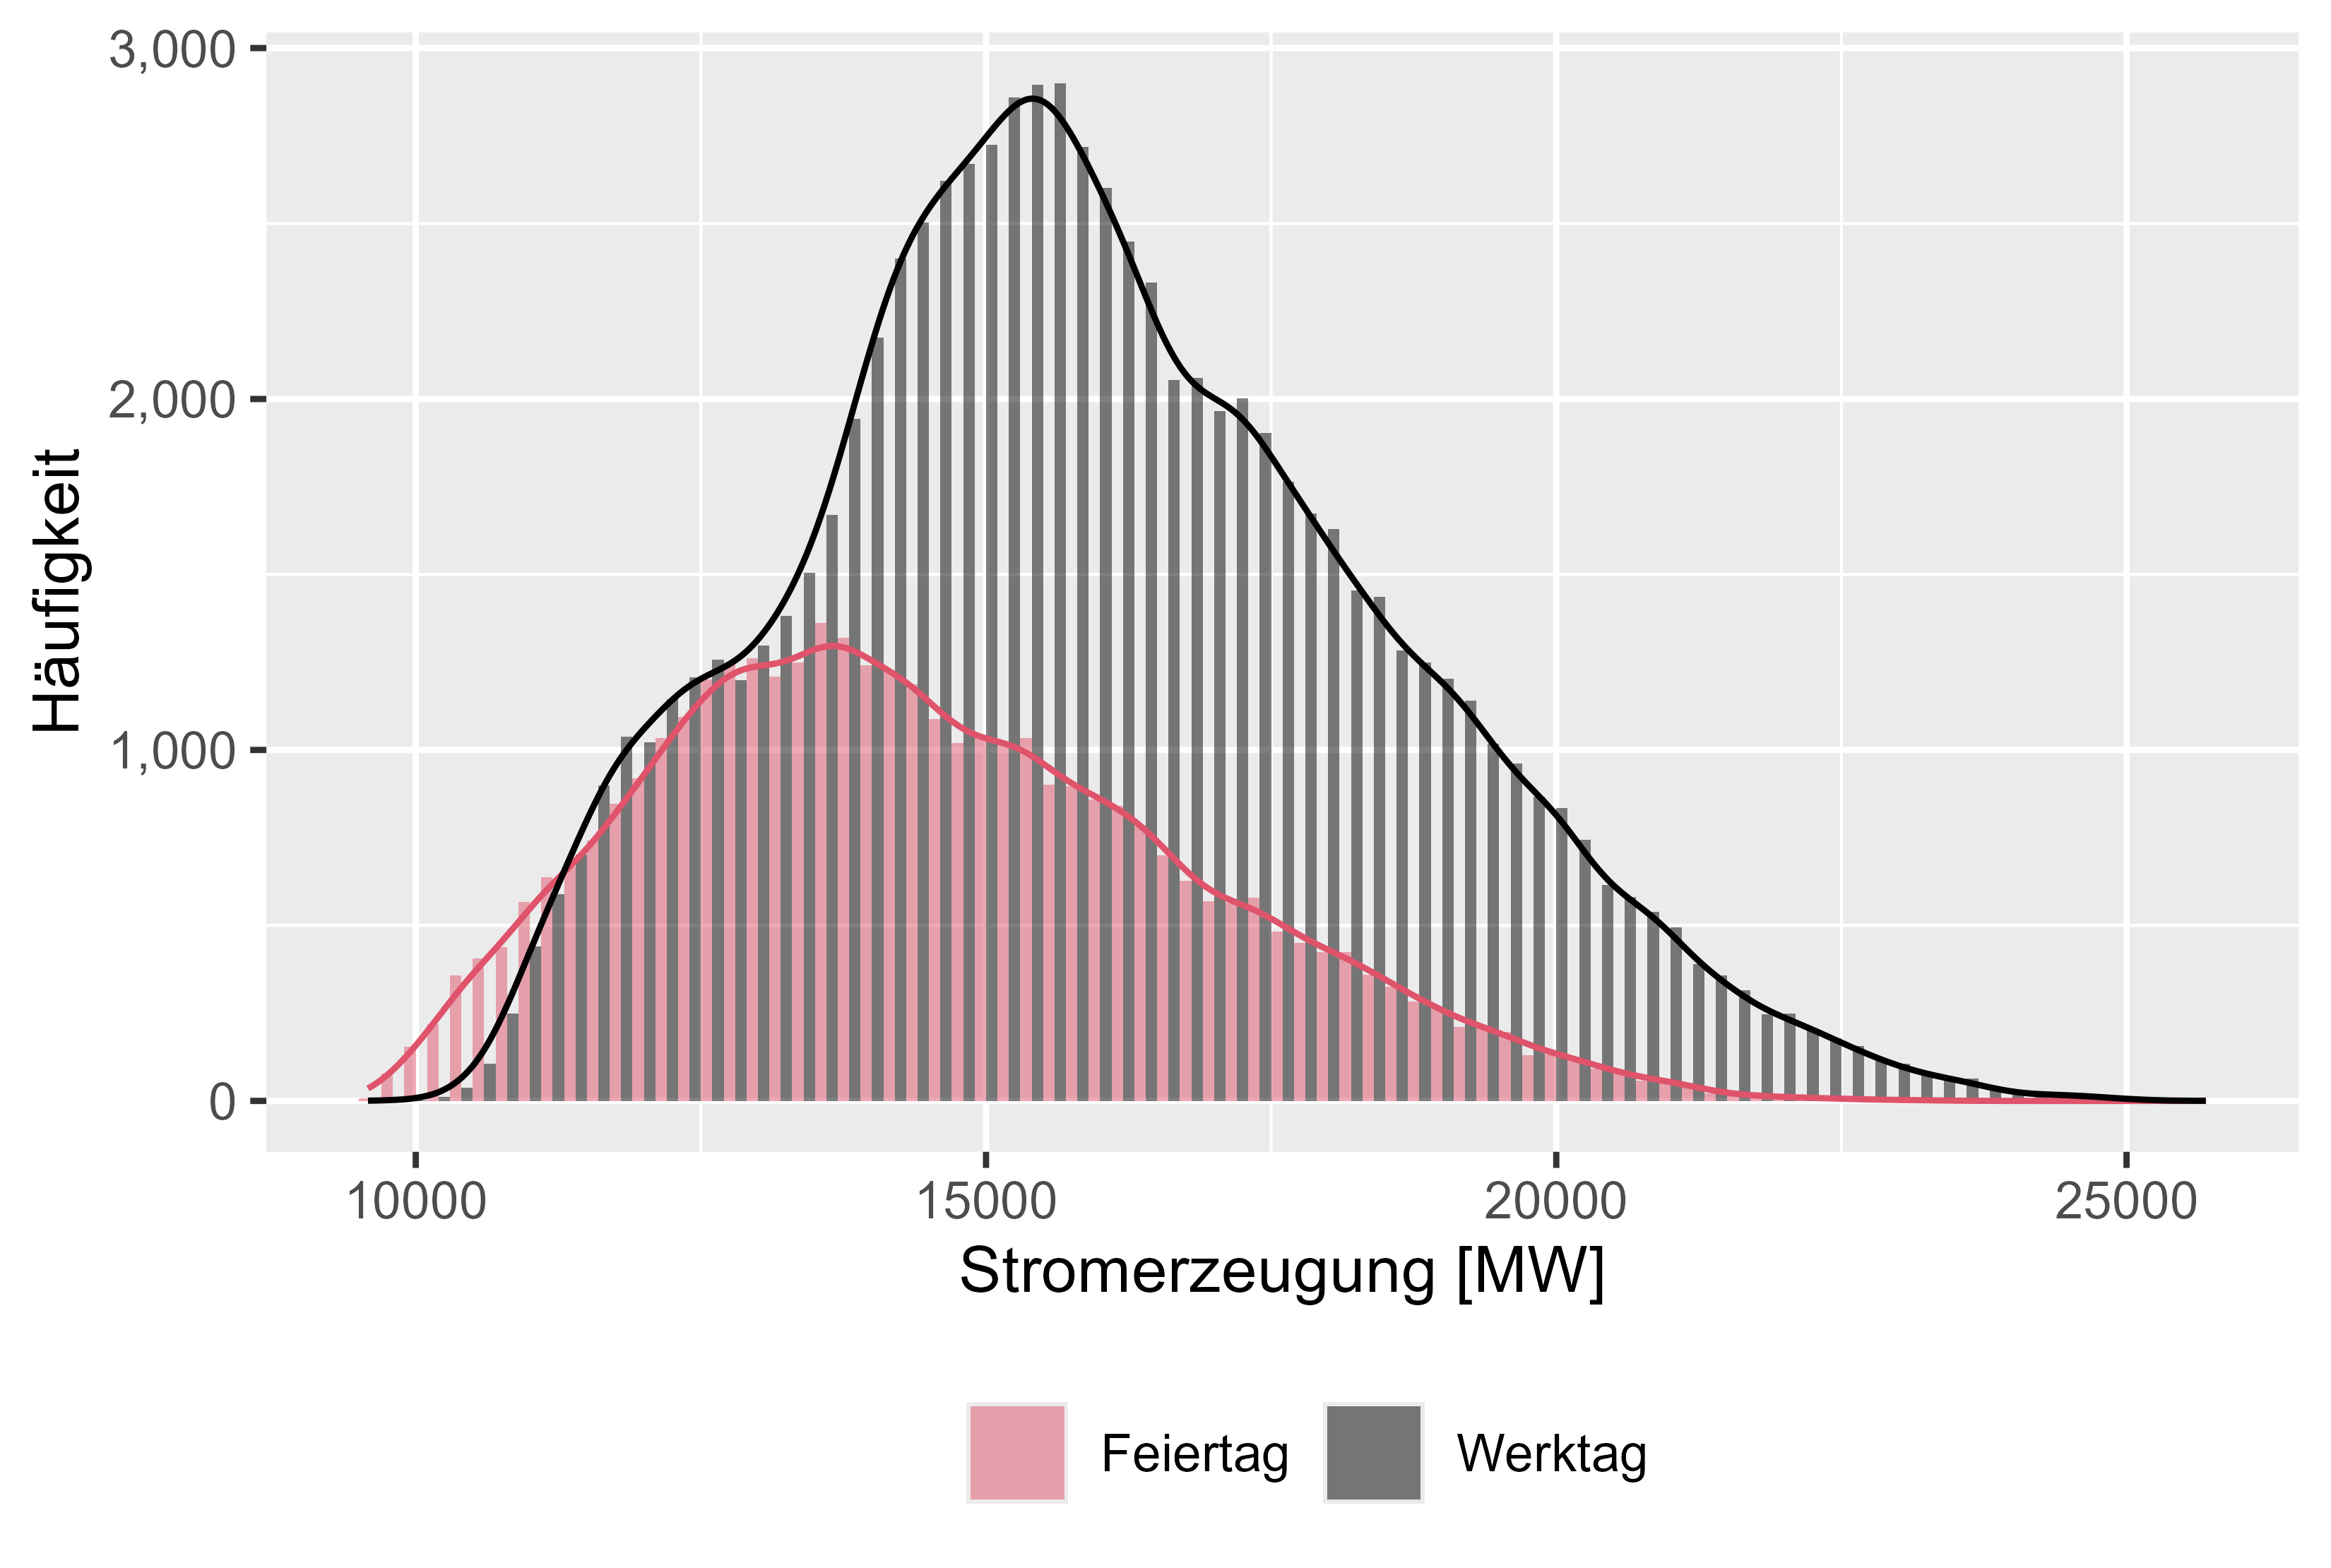
\includegraphics[width=0.7\textwidth]{plots/workday_histogram}
\caption{Verteilung der Werktage und nicht Werktage}
\label{fig:workday_histogram}
\end{figure}

Um den Begriff der komplexen Saisonalität zu verdeutlichen, zeigt die Abbildung \ref{fig:acf} die Autokorrelation. Dabei werden die aktuellen Beobachtungen mit den vergangenen gegenübergestellt und die Korrelation zwischen diesen ermittelt. So z.B. für lag 12 wird ein shift des Datensatzes um 12 Zeiteinheiten nach links verschoben. Es wird die Korrelation zwischen dem verschobenen Datensatz und dem Originalen ermittelt. So in der Abbildung \ref{fig:acf} ist eine komplexe Saisonalität abgbebildet, da es sowohl tägliche, wöchentliche als auch jährliche Muster im Datensatz zu finden sind.

\begin{figure}[H]
\centering
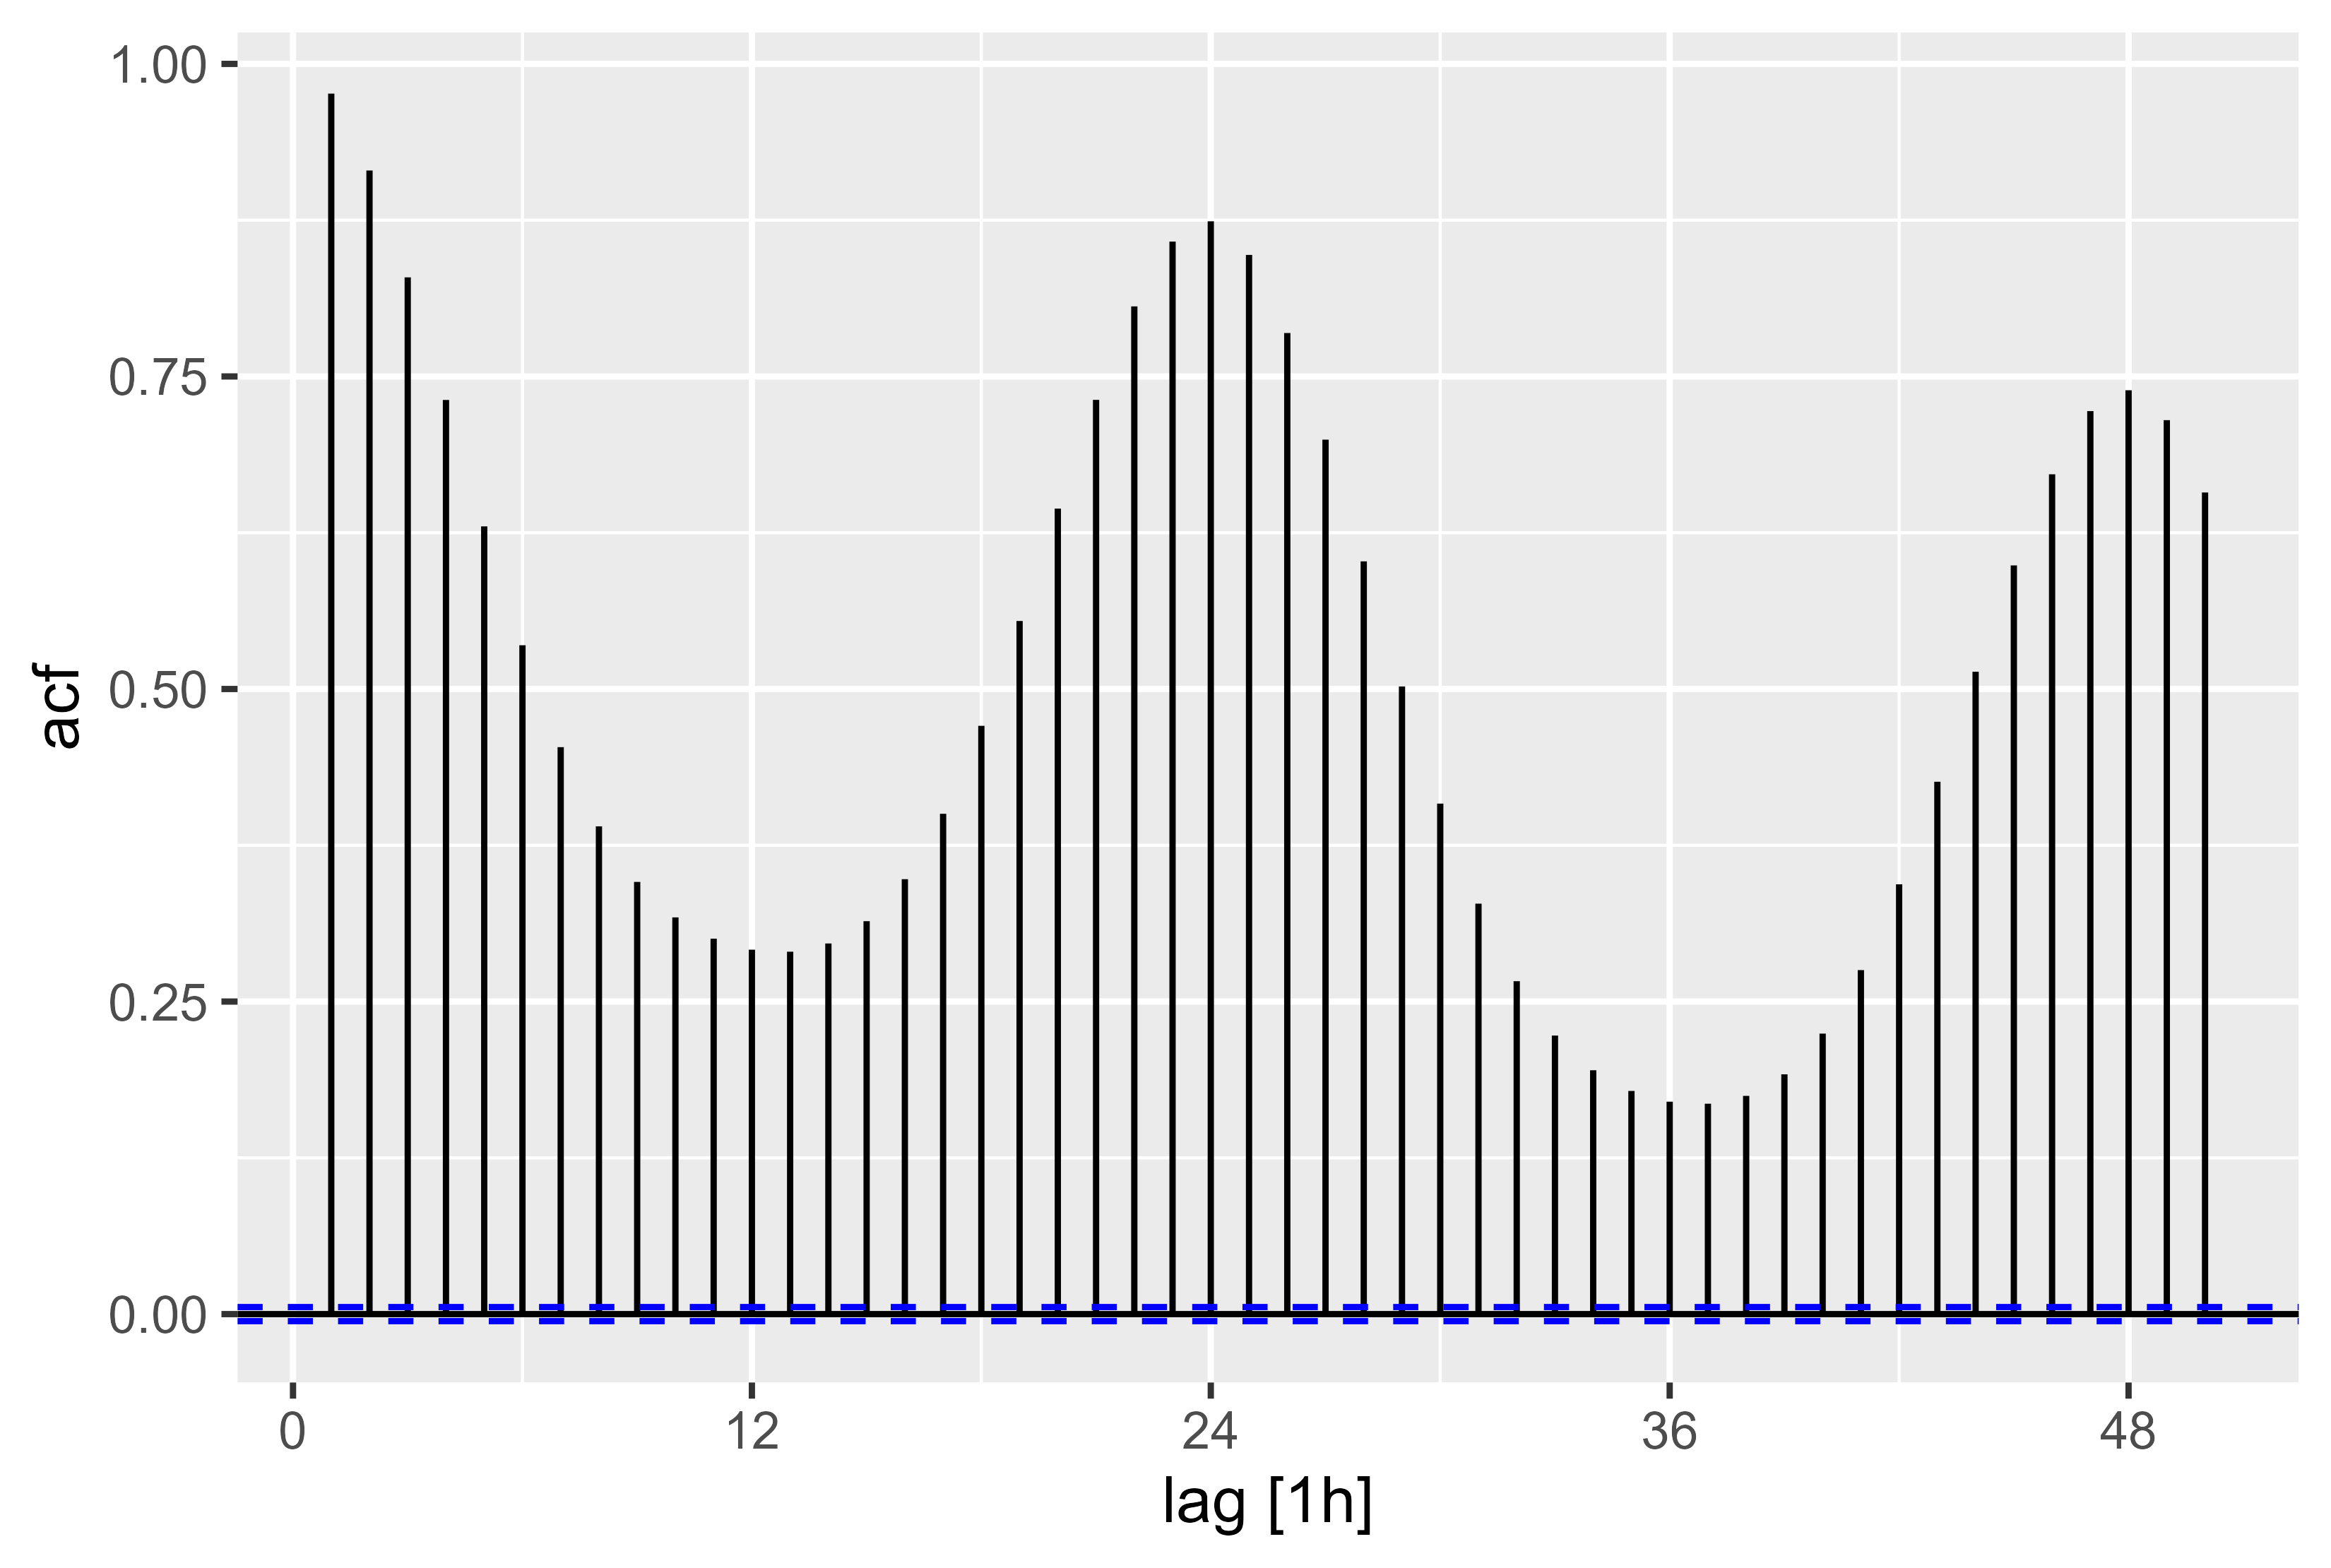
\includegraphics[width=1.0\textwidth]{plots/autocorrelation}
\caption{Autokorrelation für die Stromerzeugung}
\label{fig:acf}
\end{figure}

Als letzter Punkt in der Datenanalyse ist die Betrachtung der verschiedenen vergangenen Beobachtungen. Durchschnitt der letzten Woche, Minimum vom letzten Tag, Maximum vom letzten Tag und Durchschnitt der letzten zwei Tage. Die Abbildung \ref{fig:corr} stellt dabei die Korrelation zwischen den einzelnen Werten dar. Es ist zwischen TRUE (Werktag) und FALSE (kein Werktag) zu unterscheiden. Eine mittelstarke (ca. 0.5) Korrelation für die Stromerzeugung und die unterschiedlichen Variablen.

\begin{figure}[H]
\centering
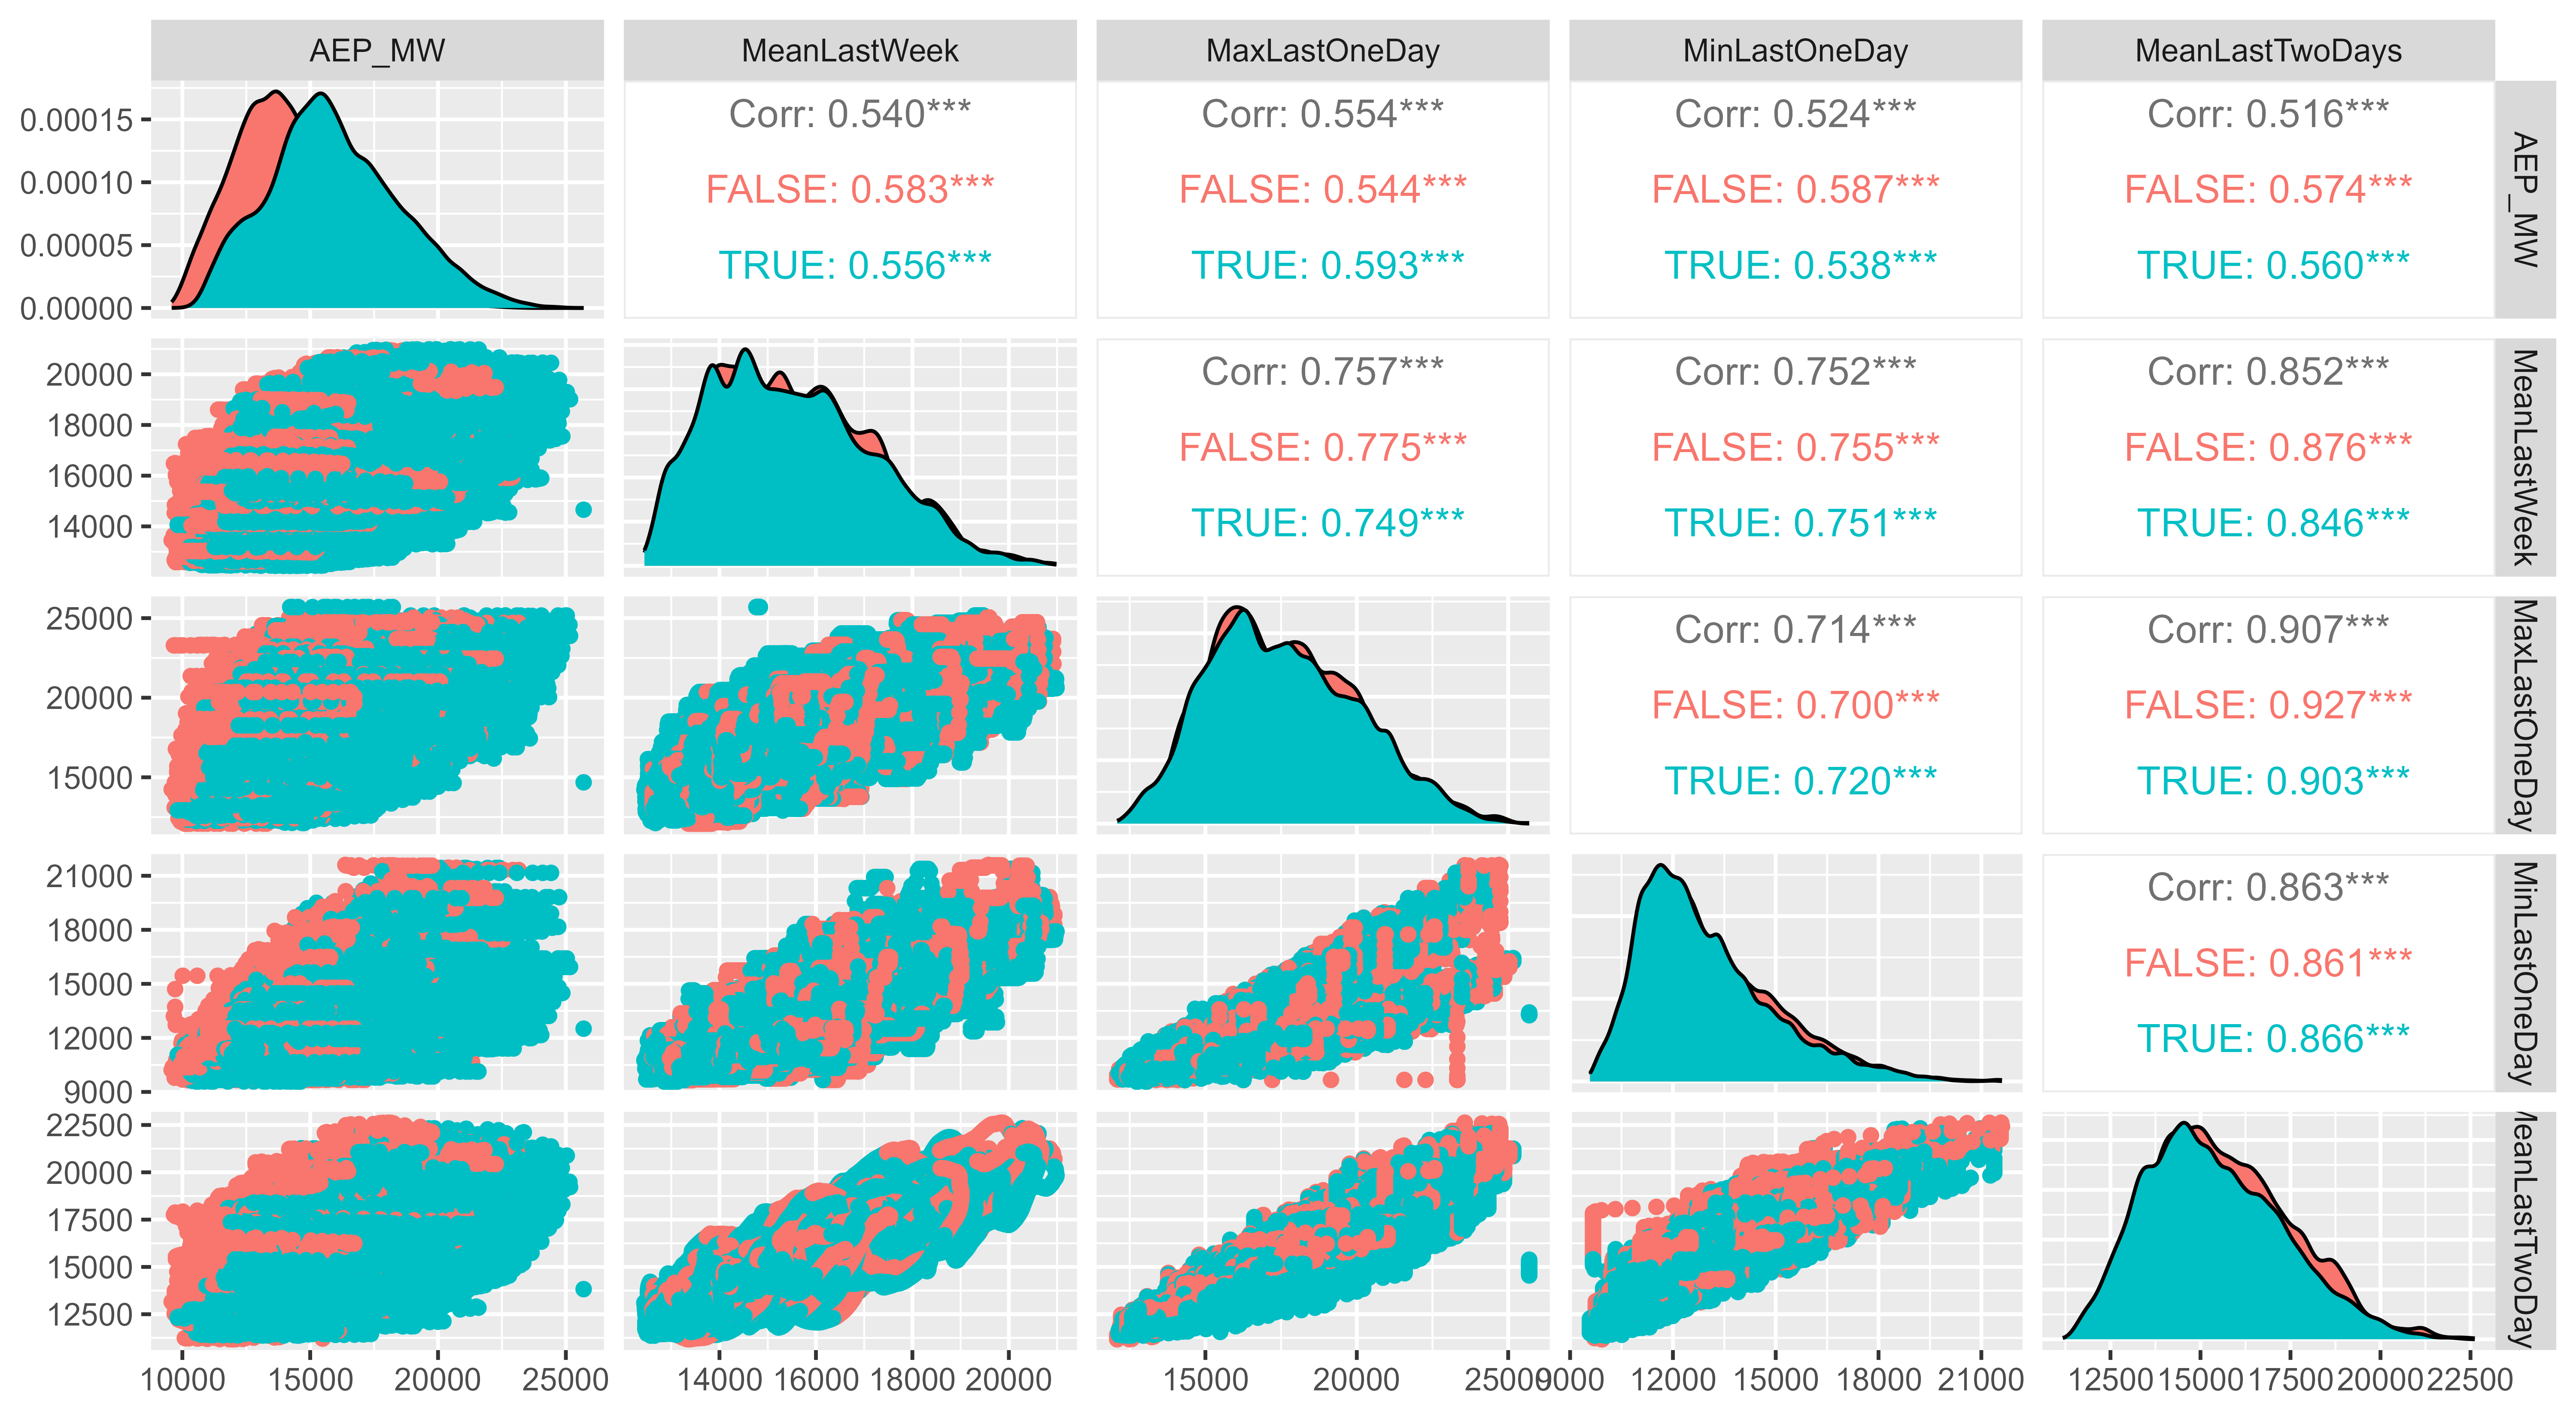
\includegraphics[width=1.0\textwidth]{plots/corr.png}
\caption{Korrelation zwischen den vergangenen Beobachtungen und der Stromerzeugung}
\label{fig:corr}
\end{figure}

Damit wurde der Datensatz nach der Analyse angepasst und kann folgend beschrieben werden:

\begin{itemize}
\tightlist
\item
  Datetime: Zeitstempel
\item
  AEP\_MW: Stromerzeugung in Megawatt
\item
  Weekday: Wochentag (Mo, Di, Mi, Do, Fr, Sa, So)
\item
  Date: Datum (YYYY-MM-DD)
\item
  Year: Jahr
\item
  Week: Kalenderwoche
\item
  Hour: Stunde
\item
  Month: Monat
\item
  WorkDay: Ob es ein Arbeitstag ist (TRUE/FALSE)
\item
  Mo: Montag (TRUE/FALSE)
\item
  Di: Dienstag (TRUE/FALSE)
\item
  Mi: Mittwoch (TRUE/FALSE)
\item
  Do: Donnerstag (TRUE/FALSE)
\item
  Fr: Freitag (TRUE/FALSE)
\item
  Sa: Samstag (TRUE/FALSE)
\item
  So: Sonntag (TRUE/FALSE)
\item
  Holiday: Ob es ein Feiertag ist (TRUE/FALSE)
\item
  LastDayWasNotWorkDay: Ob der letzte Tag kein Arbeitstag war (TRUE/FALSE)
\item
  LastDayWasNotWorkDayAndNowWorkDay: Ob der letzte Tag kein Arbeitstag war und der heutige Arbeitstag ist (TRUE/FALSE)
\item
  NextDayIsNotWorkDayAndNowWorkDay: Ob der nächste Tag kein Arbeitstag ist und der heutige Arbeitstag ist (TRUE/FALSE)
\item
  LastDayWasHolidayAndNotWeekend: Ob der letzte Tag ein Feiertag war und kein Wochenende (TRUE/FALSE)
\item
  NextDayIsHolidayAndNotWeekend: Ob der nächste Tag ein Feiertag ist und kein Wochenende (TRUE/FALSE)
\item
  HolidayName: Name des Feiertags
\item
  MeanLastWeek: Durchschnitt der letzten Woche
\item
  MeanLastTwoDays: Durchschnitt der letzten zwei Tage
\item
  MaxLastOneDay: Maximum des letzten Tages
\item
  MinLastOneDay: Minimum des letzten Tages
\end{itemize}

Anmerkung: Es wurden weitere Feature erzeugt, die z.B. den Kalender-Effekt besser beschreiben sollen. So kann es sein, dass nach einem Feiertag die Menschen Urlaub nehmen und dadurch die Stromerzeugung sinkt. So wird auch untersucht, ob der letzte Tag z.B. ein Feiertag war und nun ein Werktag.

\clearpage
\newpage

\section{Implementierung}\label{implementierung}

\subsection{SLAF Integration in LTC Nodes}\label{slaf-integration-in-ltc-nodes}

Wie schon erwähnt, die swish-Funktion wird in diesem Projekt anstatt der klassischen Sigmoid-Aktivierungsfunktion angewandt. Es wird die Funktionalität vom ``NCPs'' Package um die swish-Funktion erweitert.

Die Aktivierungsfunktion wird durch das Einstellen von dem optionalen booleschen Parameter \texttt{use\_swish\_activation} ersetzt. Bei der ``LTC'' Modelle Definition sieht der Code folgend aus:

\singlespacing

\begin{Shaded}
\begin{Highlighting}[numbers=left,,]
\KeywordTok{class}\NormalTok{ LTC(nn.Module):}
    \KeywordTok{def} \FunctionTok{\_\_init\_\_}\NormalTok{(}
        \VariableTok{self}\NormalTok{,}
\NormalTok{        input\_size: }\BuiltInTok{int}\NormalTok{,}
\NormalTok{        units,}
\NormalTok{        return\_sequences: }\BuiltInTok{bool} \OperatorTok{=} \VariableTok{True}\NormalTok{,}
\NormalTok{        batch\_first: }\BuiltInTok{bool} \OperatorTok{=} \VariableTok{True}\NormalTok{,}
\NormalTok{        mixed\_memory: }\BuiltInTok{bool} \OperatorTok{=} \VariableTok{False}\NormalTok{,}
\NormalTok{        input\_mapping}\OperatorTok{=}\StringTok{"affine"}\NormalTok{,}
\NormalTok{        output\_mapping}\OperatorTok{=}\StringTok{"affine"}\NormalTok{,}
\NormalTok{        ode\_unfolds}\OperatorTok{=}\DecValTok{6}\NormalTok{,}
\NormalTok{        epsilon}\OperatorTok{=}\FloatTok{1e{-}8}\NormalTok{,}
\NormalTok{        implicit\_param\_constraints}\OperatorTok{=}\VariableTok{True}\NormalTok{,}
\NormalTok{        use\_swish\_activation}\OperatorTok{=}\VariableTok{False}\NormalTok{,}
\NormalTok{    ):}
\NormalTok{      ...}
\end{Highlighting}
\end{Shaded}

Der Parameter wird später in jede LTC Knoten übergeben, welcher durch eine weitere Python Klasse repräsentiert wird:

\singlespacing

\begin{Shaded}
\begin{Highlighting}[numbers=left,,]
\KeywordTok{class}\NormalTok{ LTCCell(nn.Module):}
    \KeywordTok{def} \FunctionTok{\_\_init\_\_}\NormalTok{(}
        \VariableTok{self}\NormalTok{,}
\NormalTok{        wiring,}
\NormalTok{        in\_features}\OperatorTok{=}\VariableTok{None}\NormalTok{,}
\NormalTok{        input\_mapping}\OperatorTok{=}\StringTok{"affine"}\NormalTok{,}
\NormalTok{        output\_mapping}\OperatorTok{=}\StringTok{"affine"}\NormalTok{,}
\NormalTok{        ode\_unfolds}\OperatorTok{=}\DecValTok{6}\NormalTok{,}
\NormalTok{        epsilon}\OperatorTok{=}\FloatTok{1e{-}8}\NormalTok{,}
\NormalTok{        implicit\_param\_constraints}\OperatorTok{=}\VariableTok{False}\NormalTok{,}
\NormalTok{        use\_swish\_activation}\OperatorTok{=}\VariableTok{False}\NormalTok{,}
\NormalTok{    ):}
\NormalTok{      ...}
\end{Highlighting}
\end{Shaded}

Falls der Parameter als True gesetzt ist, wird ein neuer Parameter für PyTorch Modelle definiert, welcher ein zufälliger Skalarwert im Zahlenbereich von \texttt{0,5} bis \texttt{1,5} ist:

\singlespacing

\begin{Shaded}
\begin{Highlighting}[numbers=left,,]
\KeywordTok{def}\NormalTok{ add\_weight(}\VariableTok{self}\NormalTok{, name, init\_value, requires\_grad}\OperatorTok{=}\VariableTok{True}\NormalTok{):}
\NormalTok{    param }\OperatorTok{=}\NormalTok{ torch.nn.Parameter(init\_value, requires\_grad}\OperatorTok{=}\NormalTok{requires\_grad)}
    \VariableTok{self}\NormalTok{.register\_parameter(name, param)}
    \ControlFlowTok{return}\NormalTok{ param}

\KeywordTok{def}\NormalTok{ \_get\_init\_value(}\VariableTok{self}\NormalTok{, shape, param\_name):}
\NormalTok{    minval, maxval }\OperatorTok{=} \VariableTok{self}\NormalTok{.\_init\_ranges[param\_name]}
    \ControlFlowTok{if}\NormalTok{ minval }\OperatorTok{==}\NormalTok{ maxval:}
        \ControlFlowTok{return}\NormalTok{ torch.ones(shape) }\OperatorTok{*}\NormalTok{ minval}
    \ControlFlowTok{else}\NormalTok{:}
        \ControlFlowTok{return}\NormalTok{ torch.rand(}\OperatorTok{*}\NormalTok{shape) }\OperatorTok{*}\NormalTok{ (maxval }\OperatorTok{{-}}\NormalTok{ minval) }\OperatorTok{+}\NormalTok{ minval}

\ControlFlowTok{if} \VariableTok{self}\NormalTok{.\_use\_swish\_activation:}
    \VariableTok{self}\NormalTok{.\_params[}\StringTok{"swish\_beta"}\NormalTok{] }\OperatorTok{=} \VariableTok{self}\NormalTok{.add\_weight(}
        \StringTok{"swish\_beta"}\NormalTok{,}
\NormalTok{        init\_value}\OperatorTok{=}\VariableTok{self}\NormalTok{.\_get\_init\_value(}
\NormalTok{            (}\DecValTok{1}\NormalTok{,), }\StringTok{"swish\_beta"}
\NormalTok{        ),}
\NormalTok{    )}
\end{Highlighting}
\end{Shaded}

Der Skalar wird dann später verwendet, um ein Matrizen Produkt zu berechnen:

\singlespacing

\begin{Shaded}
\begin{Highlighting}[numbers=left,,]
\KeywordTok{def}\NormalTok{ \_sigmoid(}\VariableTok{self}\NormalTok{, v\_pre, mu, sigma, beta):}
\NormalTok{    v\_pre }\OperatorTok{=}\NormalTok{ torch.unsqueeze(v\_pre, }\OperatorTok{{-}}\DecValTok{1}\NormalTok{)  }\CommentTok{\# For broadcasting}
\NormalTok{    mues }\OperatorTok{=}\NormalTok{ v\_pre }\OperatorTok{{-}}\NormalTok{ mu}
\NormalTok{    x }\OperatorTok{=}\NormalTok{ sigma }\OperatorTok{*}\NormalTok{ mues}
    \ControlFlowTok{if} \VariableTok{self}\NormalTok{.\_use\_swish\_activation:}
        \ControlFlowTok{return}\NormalTok{ x }\OperatorTok{*}\NormalTok{ torch.sigmoid(beta }\OperatorTok{*}\NormalTok{ x)}
    \ControlFlowTok{return}\NormalTok{ torch.sigmoid(x)}
\end{Highlighting}
\end{Shaded}

Der Parameter (swish beta) wird während des Trainings kontinuierlich verändert. Das passiert wenn die Fehler ins Netz zurückgespielt werden.

\clearpage
\newpage

\subsection{Feature Engineering}\label{feature-engineering}

Neben den initialen Variablen, die aus der Datenanalyse erzeugt wurden, werden zwei weitere Spalten hinzugefügt. Nämlich die wöchentliche und jährliche Verzögerung der abhängigen Variable. Für Time-Series Daten ist es eine normale Praktik, die wir hier auch verfolgen. Somit ergeben sich ca. 30 Features, die einen möglichen Einfluss auf das Modell haben können.

\begin{itemize}
\tightlist
\item
  x: \(x_{t-24}\) Verschiebung um einen Tag zurück.
\item
  x\_shifted\_week: \(x_{t-24*7}\) Verschiebung um eine Woche zürück.
\item
  x\_shifted\_year: \(x_{t-24*365}\) Verschiebung um ein Jahr zürück.
\end{itemize}

Wegen dieser großen Dimensionalität des Datensatzes möchten wir mithilfe der PCA-Analyse zeigen, wie viele Variablen benötigt werden, um die Varianz der Daten zu erklären. Folgend eine Tabelle, wie viele Komponenten gebraucht werden, um die Varianz des Datensatzes zu beschreiben:

\begin{table}[h!]
\centering
\begin{tabularx}{\textwidth}{|c|c|X|}
\hline
\textbf{Principal Component} & \textbf{Merkmal}                        & \textbf{Kummulierte Varianz} \\ \hline
\textbf{PC1}                 & x                                      & 0.61522145                              \\ \hline
\textbf{PC2}                 & x\_shifted\_week                       & 0.80951859                              \\ \hline
\textbf{PC3}                 & x\_shifted\_year                       & 0.86591735                              \\ \hline
\textbf{PC4}                 & MaxLastOneDay                          & 0.90337726                              \\ \hline
\textbf{PC5}                 & WorkDay                                & 0.9391192                               \\ \hline
\textbf{PC6}                 & MeanLastWeek                           & 0.96688936                              \\ \hline
\textbf{PC7}                 & MinLastOneDay                          & 0.98807356                              \\ \hline
\textbf{PC8}                 & MeanLastTwoDays                        & 0.99384472                              \\ \hline
\textbf{PC9}                 & LastDayWasHolidayAndNotWeekend         & 0.99713582                              \\ \hline
\textbf{PC10}                & NextDayIsHolidayAndNotWeekend          & 1.0                                     \\ \hline
\end{tabularx}
\caption{PCA: Beschreibung der Varianz}
\label{table:pc_explained_variance}
\end{table}

Die Komponenten sind in der Reihenfolge nach deren Wichtigkeit (Feature Importance) platziert. Jedoch zeigt die Tabelle, dass die numerischen Variablen höher platziert sind als die booleschen Merkmale, weil diese stärkere Korrelation mit abhängigen Variablen aufweisen.

Trotzdem hat sich im Verlauf des Trainings herausgestellt, dass die verzögerten Werte eher das Modell verwirren als fördern. Aufgrund des enormen Zeitaufwands, um alle Möglichkeiten der ca. 30 Features durchzugehen (Grid-Search für Features) wurde in dieser Arbeit
der Ansatz der Datenanalyse verfolgt. Dabei wurde versucht, logisch die Variablen herauszupicken und ins Modell hereinfließen zu lassen. Das Ganze untermauert mit der Datenanalyse. Im folgenden Unterkapitel beschreibt die \texttt{FEATURES\_LIST} die ausgewählten Features. Dabei war es auch die Idee für den Anfang einen etwas einfacheren Ansatz zu untersuchen.

\subsection{Training}\label{training}

Durch die \texttt{pytorch}-Implementierung lässt sich das Training sowohl auf einer CPU als auch einer GPU ohne große Anpassungen laufen lassen. Um das Training stabiler zu gestalten, wurde die Hardware vom FH-SWF Cluster genutzt.

Das Training lässt sich sowohl mittels des cmd-Befehl als auch Jupyter Notebook anstoßen, allein nur die Parameter in \texttt{config.py} sind entscheidend:

\clearpage
\newpage

\singlespacing

\begin{Shaded}
\begin{Highlighting}[numbers=left,,]
\NormalTok{PATH }\OperatorTok{=} \StringTok{"data/csv/AEP\_hourly\_cleaned.csv"}
\NormalTok{STATION }\OperatorTok{=} \StringTok{"AEP\_MW"}
\NormalTok{FEATURES\_LIST }\OperatorTok{=}\NormalTok{ [}
    \StringTok{"WorkDay"}\NormalTok{,}
    \StringTok{"LastDayWasHolodiayAndNotWeekend"}\NormalTok{,}
    \StringTok{"NextDayIsHolidayAndNotWeekend"}\NormalTok{,}
    \StringTok{"MeanLastWeek"}\NormalTok{,}
    \StringTok{"MeanLastTwoDays"}\NormalTok{,}
    \StringTok{"MaxLastOneDay"}\NormalTok{,}
    \StringTok{"MinLastOneDay"}
\NormalTok{]}
\NormalTok{FEATURES\_2\_SCALE }\OperatorTok{=}\NormalTok{ [}
    \StringTok{"value"}\NormalTok{,}
    \StringTok{"MeanLastWeek"}\NormalTok{,}
    \StringTok{"MeanLastTwoDays"}\NormalTok{,}
    \StringTok{"MaxLastOneDay"}\NormalTok{,}
    \StringTok{"MinLastOneDay"}
\NormalTok{]}

\NormalTok{YEAR\_SHIFT }\OperatorTok{=} \DecValTok{365}
\NormalTok{WEEK\_SHIFT }\OperatorTok{=} \DecValTok{7}
\NormalTok{VALUES\_PER\_DAY }\OperatorTok{=} \DecValTok{24}
\NormalTok{FILTER\_DT\_FROM }\OperatorTok{=} \StringTok{"2014{-}01{-}01 00:00:00"}
\NormalTok{FILTER\_DT\_TILL }\OperatorTok{=} \StringTok{"2017{-}01{-}01 00:00:00"}

\NormalTok{GRID\_SEARCH }\OperatorTok{=} \VariableTok{True}

\NormalTok{BATCH\_SIZE }\OperatorTok{=} \DecValTok{7}
\NormalTok{NUM\_WORKERS }\OperatorTok{=} \DecValTok{128}
\NormalTok{NUM\_LNN\_UNITS }\OperatorTok{=}\NormalTok{ [}\DecValTok{16}\NormalTok{, }\DecValTok{8}\NormalTok{, }\DecValTok{32}\NormalTok{]}

\NormalTok{USE\_SWISH\_ACTIVATION }\OperatorTok{=}\NormalTok{ [}\VariableTok{False}\NormalTok{, }\VariableTok{True}\NormalTok{]}
\NormalTok{INIT\_LR }\OperatorTok{=}\NormalTok{ [}\FloatTok{0.01}\NormalTok{, }\FloatTok{0.0001}\NormalTok{]}
\NormalTok{NUM\_EPOCHS }\OperatorTok{=}\NormalTok{ [}\DecValTok{10}\NormalTok{]}
\end{Highlighting}
\end{Shaded}

Außer Datenpfad, Energiestation und Liste relevanter Features lässt sich auch einen Grid Search mit dem Parameter-Pool einstellen. Die wichtigsten Hyperparameter, die für LNN eine Rolle spielen, sind die Anzahl von Knoten, eine initiale Learning-Rate und die Anzahl von Epochen.
In der Konfiguration werden auch die Schranken für den Trainingsdatensatz definiert. In diesem Fall war es sinnvoll, die letzten 3 Jahre zum Vorhersagejahr zu nehmen (hier 2014 und 2017). Dies ist damit zu begründen, dass das Modell sowohl das jährliche Muster, wöchentliche Muster als auch das tägliche Muster lernen soll.

Bevor das eigentliche Training startet, werden die Daten im Bereich zwischen 0 und 1 mit dem \texttt{sklearn.processing.MinMaxScaler} Objekt normalisiert. Für die Evaluation der Ergebnisse bzw. produktives Nutzen kann der Scaler die Daten denormalisieren. Welche Features normalisiert werden, wird mittels \texttt{FEATURES\_2\_SCALE} eingestellt, da z.B. die booleschen Variablen keine Skalierung brauchen.

Für das unkomplizierte Training wird die \texttt{Trainer} Klasse aus der \texttt{pytorch\_lightning} Bibliothek benutzt, welche einen Data Scientisten vom Boiler Code befreit.

Der Grid Search für die Parameter wurde auf 10 Epochen pro Parameterkombination begrenzt, um das Potenzial von den Modellen analytisch zur 10-ten Epoche zu betrachten. Dafür wurden insgesamt 36 Modelle miteinander verglichen. Zuerst wurde für jeden Kandidaten ein \texttt{Mean\ Average\ Percentage\ Error} berechnet und eine grafische Darstellung der Vorhersagen als ein Anhaltspunkt genommen. Die meist vielversprechenden Parameterkombinationen wurden dann für längeres Training (100 Epochen) ausgewählt.

Nach 10 Epochen hatten die besten Modelle einen \texttt{MAPE\ Loss} zwischen 19\% und 25\% gezeigt:

\begin{figure}[H]
\centering
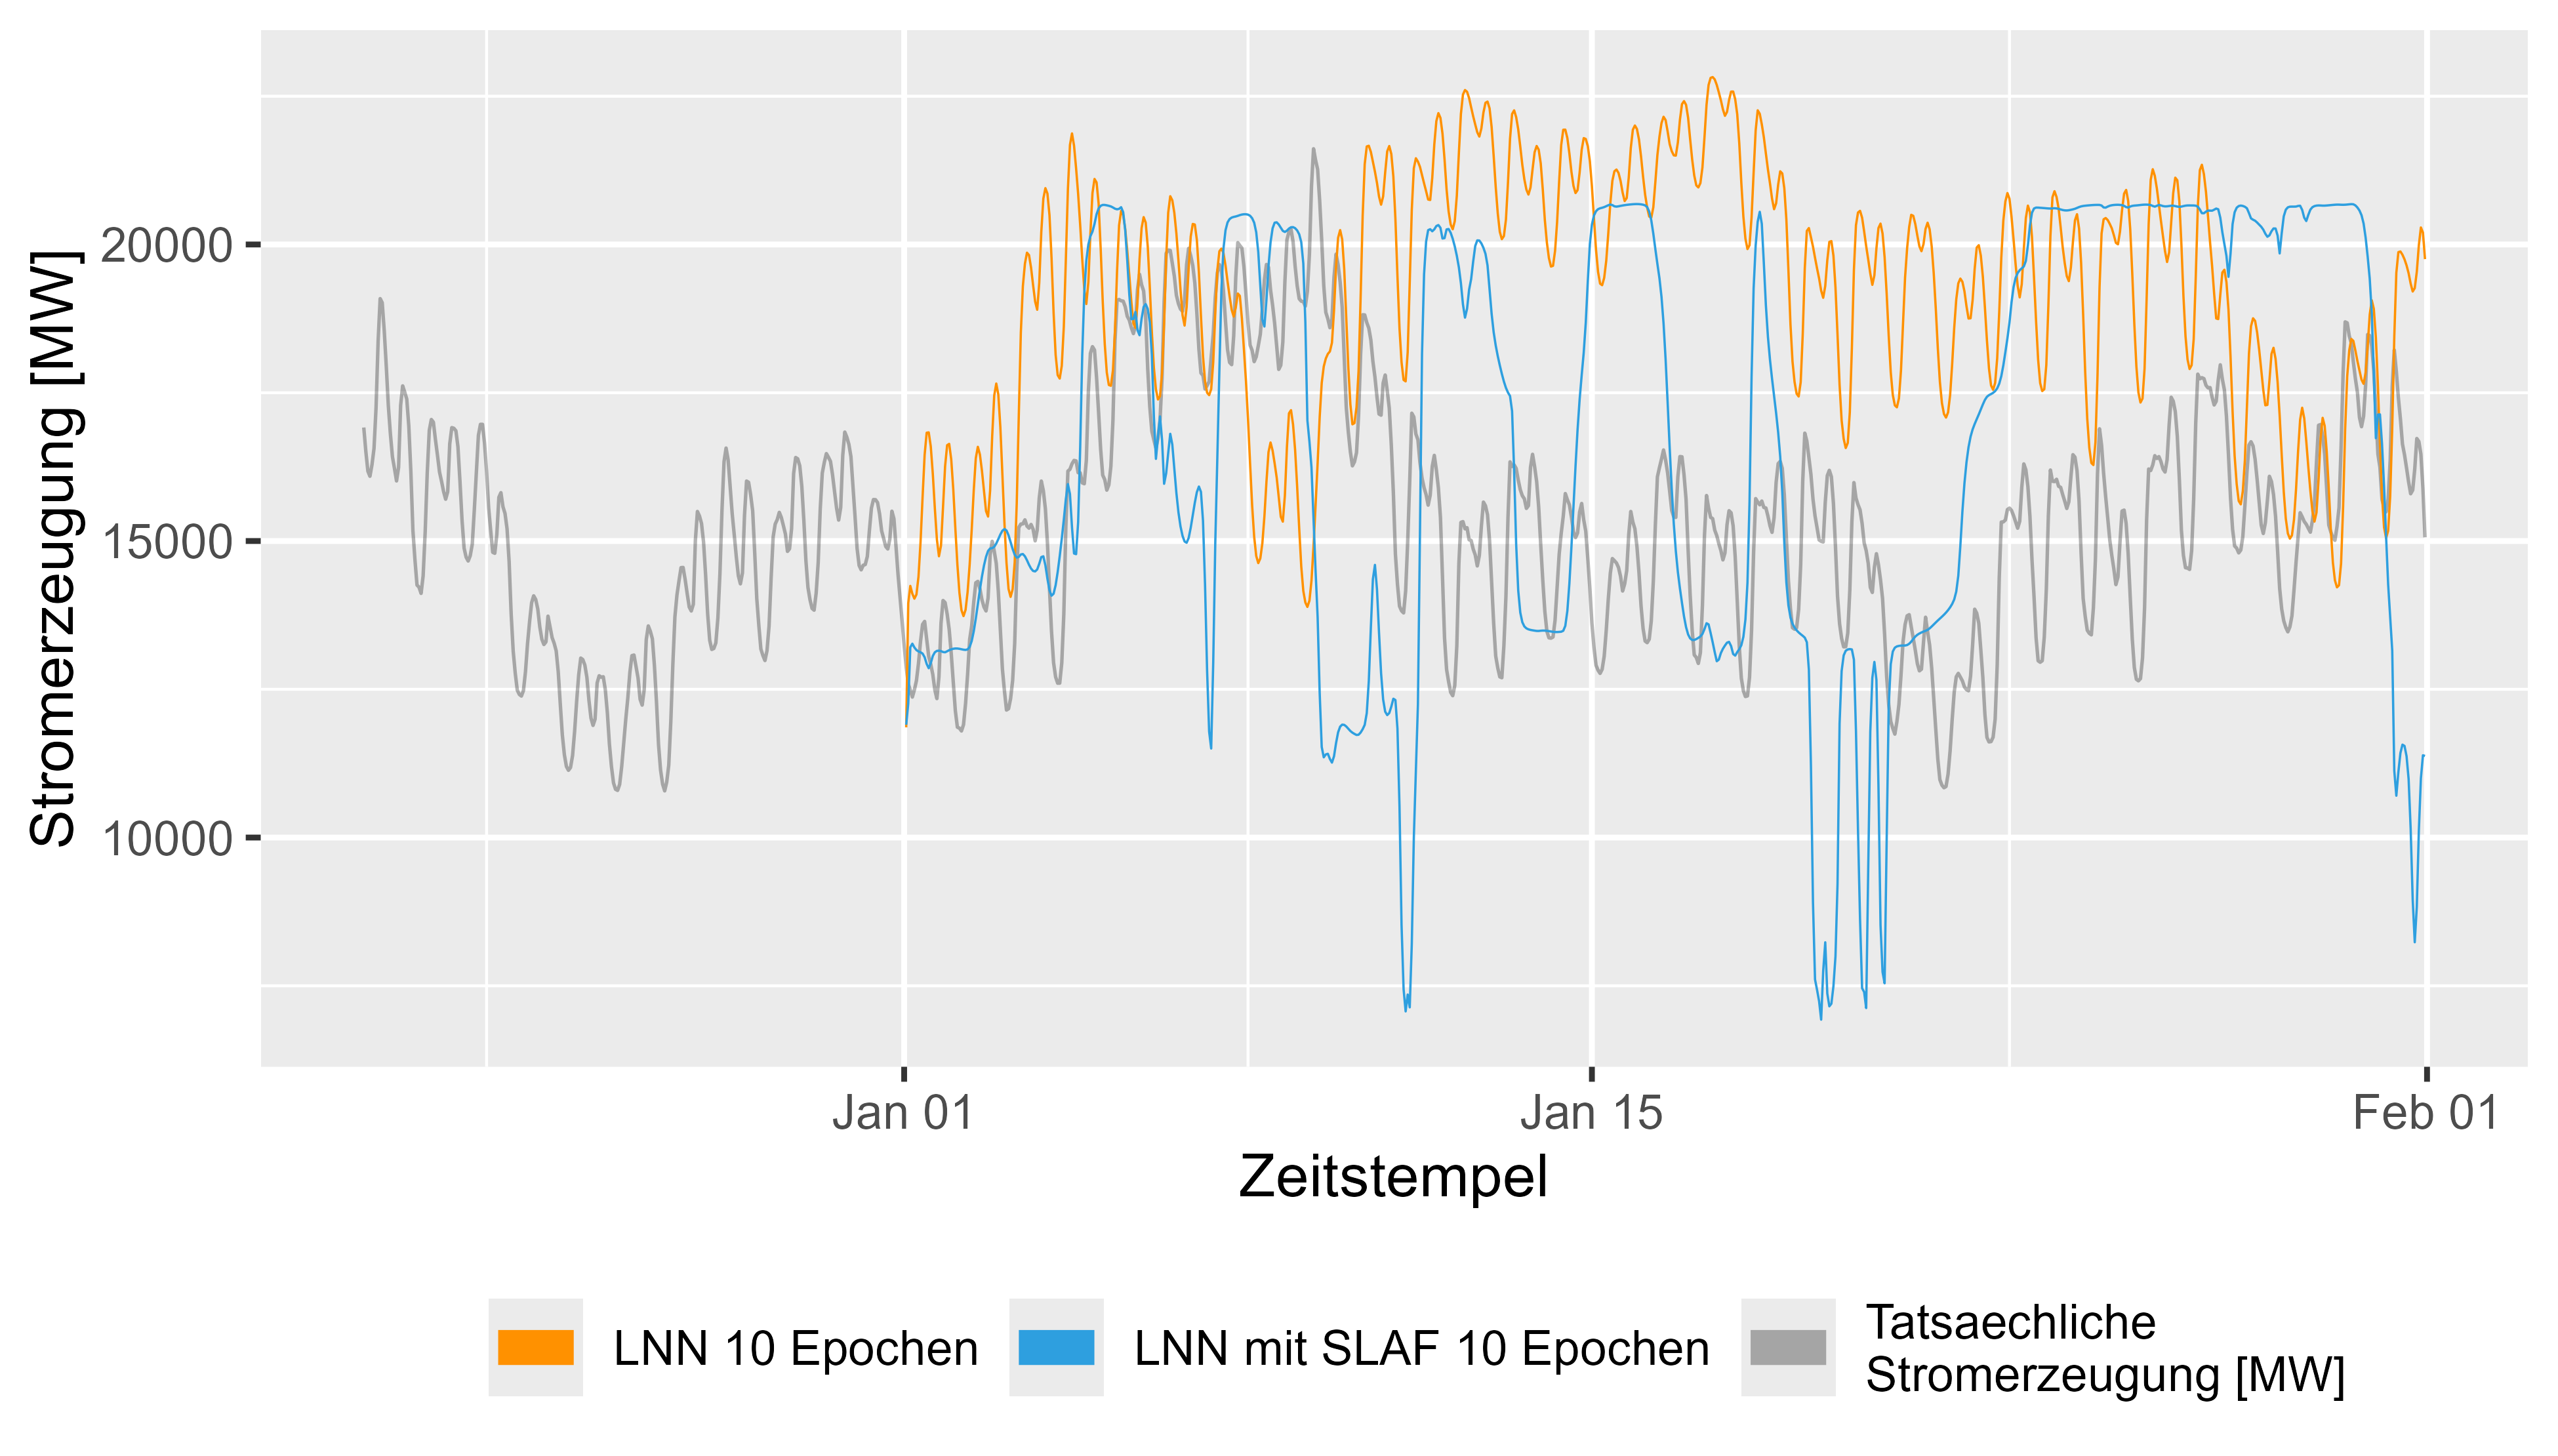
\includegraphics[width=1.0\textwidth]{plots/10_epochs_cobmined_nnLNN mit SLAF 10 Epochen.png}
\caption{Nach 10 Epochen mit und ohne SLAF, Ausschnitt für Januar}
\label{fig:slaf_lnn_10_epochs_january}
\end{figure}

\begin{figure}[H]
\centering
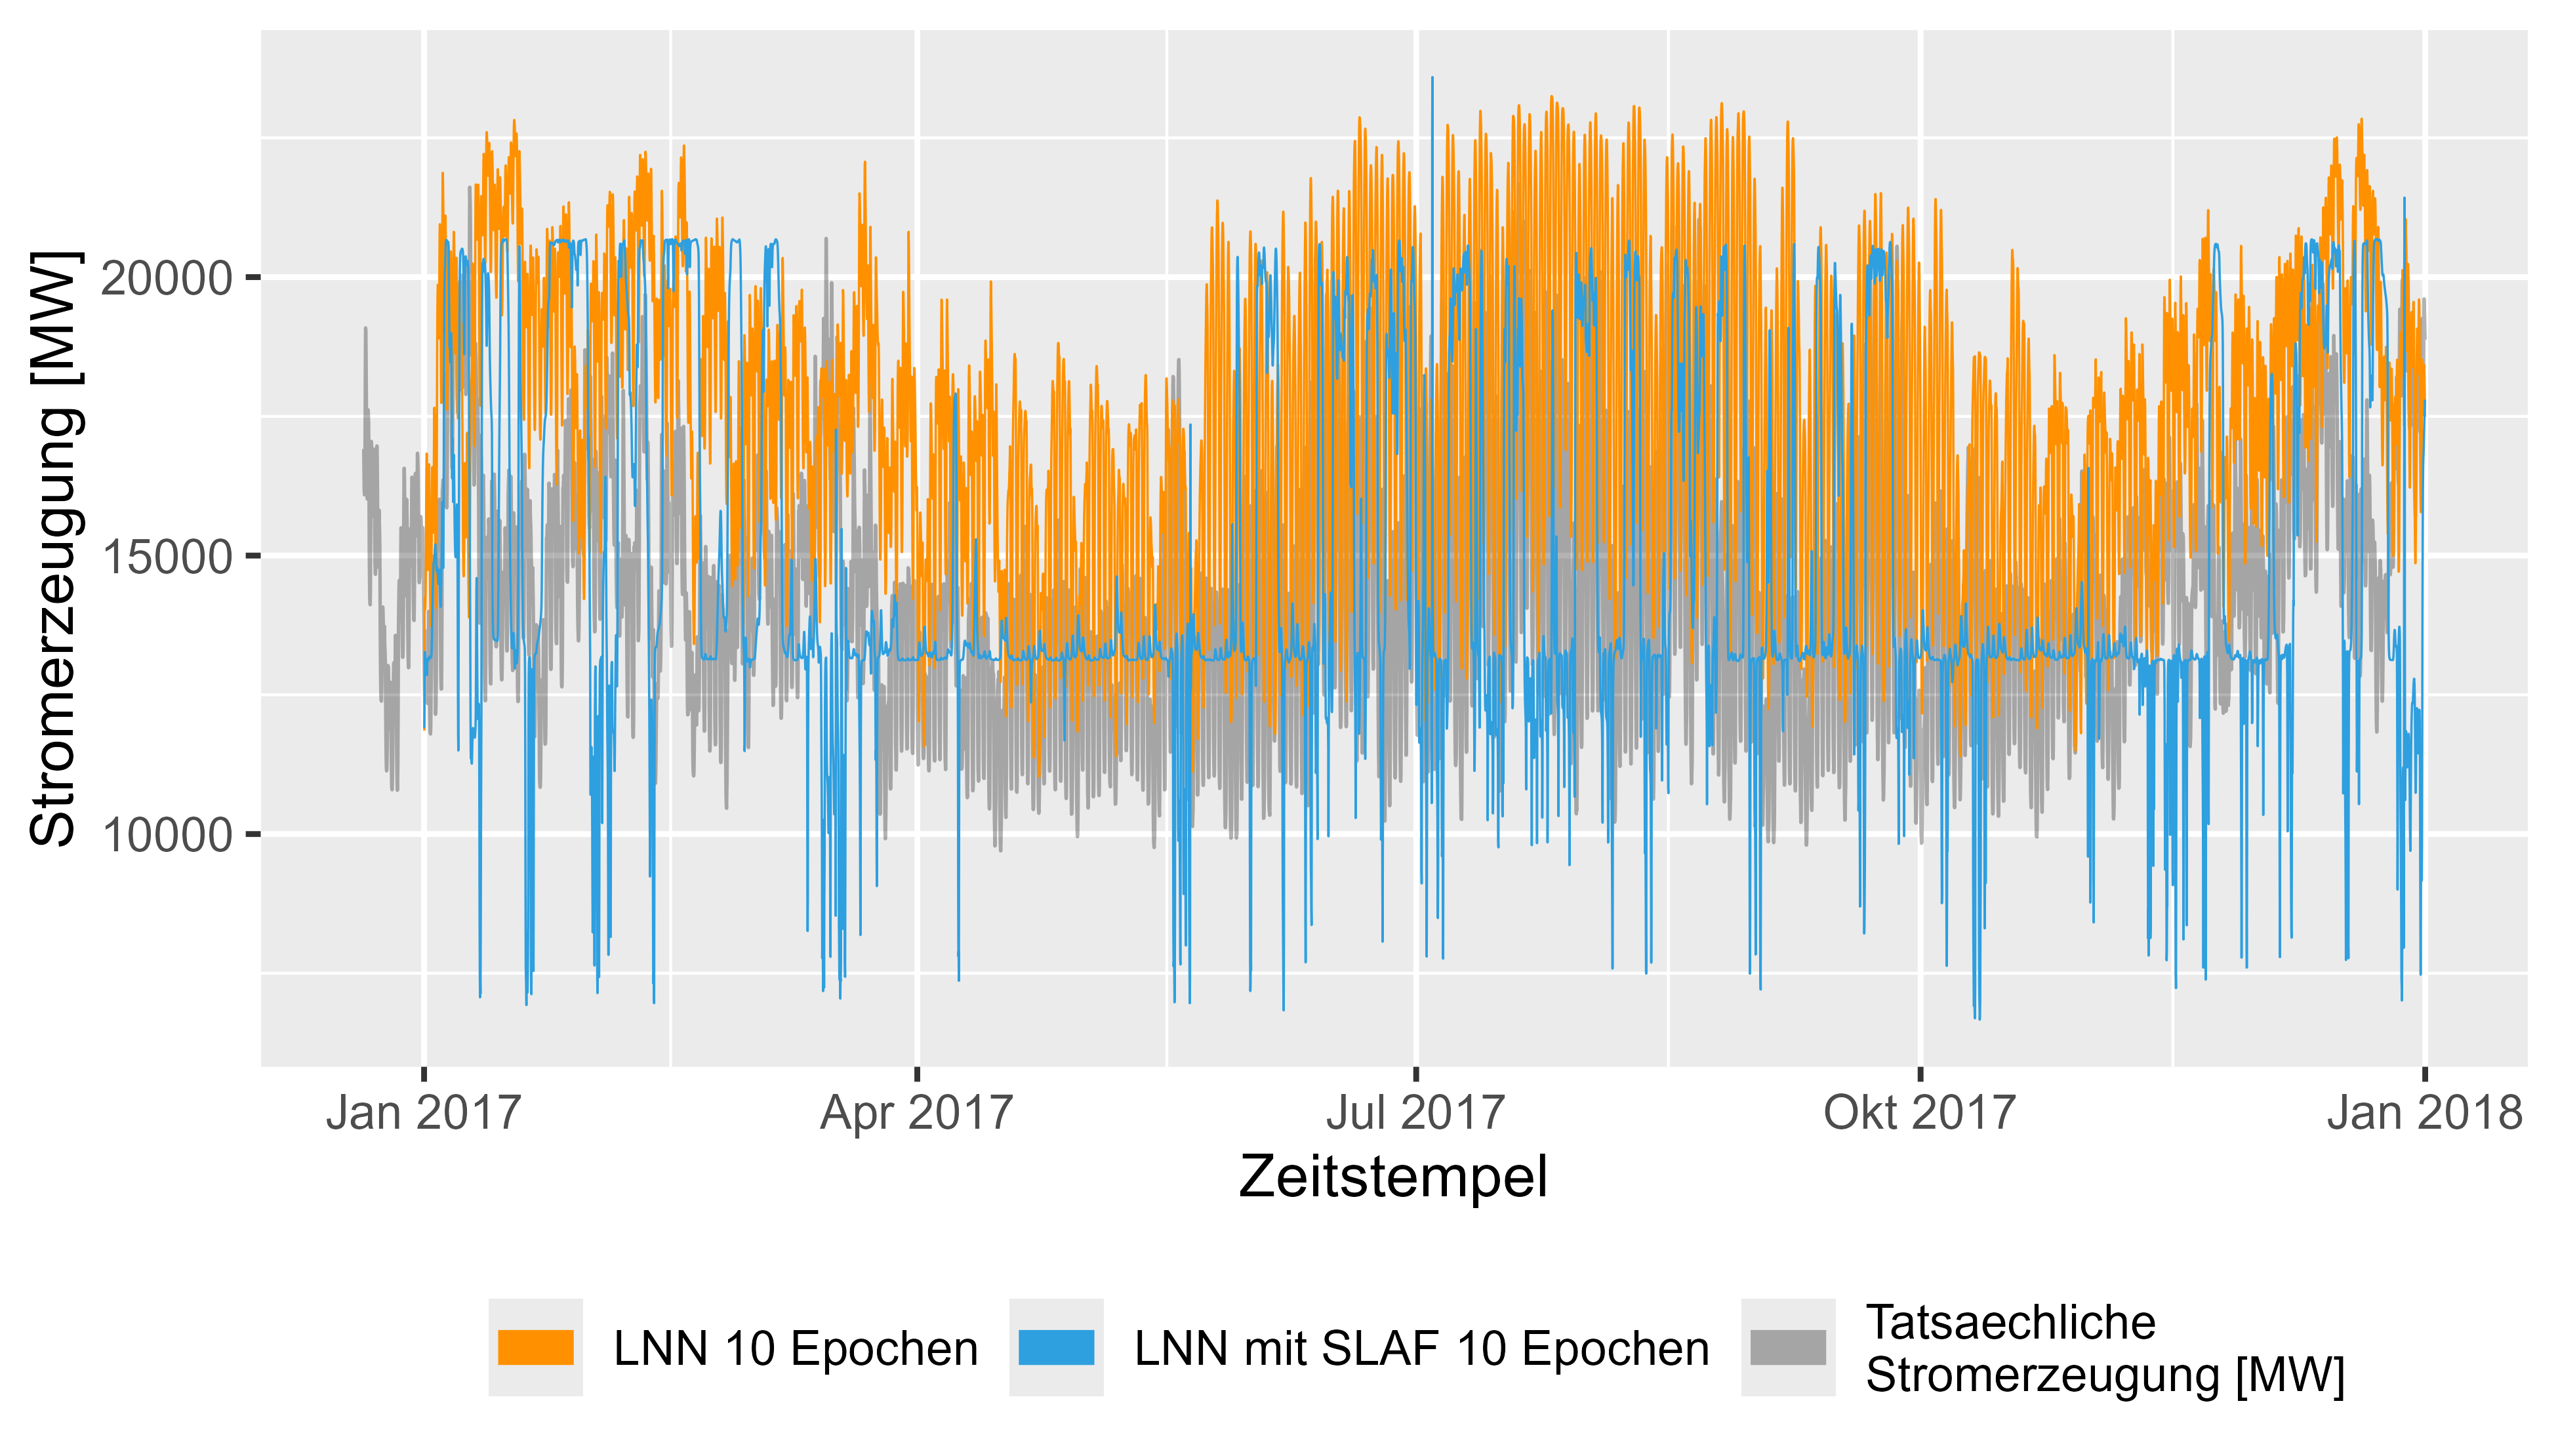
\includegraphics[width=1.0\textwidth]{plots/10_epochs_all_time_cobmined_nnLNN mit SLAF 10 Epochen.png}
\caption{Nach 10 Erpochen mit und ohne SLAF, ganzes Jahr 2017}
\label{fig:slaf_lnn_10_epochs_2017}
\end{figure}

\clearpage
\newpage

\section{Vorhersage Ergebnisse}\label{vorhersage-ergebnisse}

Ein Vergleichskriterium für die verschiedenen Modelle ist der MAPE. Es wurden verschiedene statistische Modelle und Methoden implementiert und ausprobiert. ARIMA Modell, NAIVE Methode, MEAN Methode, DRIFT Methode und das Prophet-Modell. Alle Modelle wurden vereinfacht implementiert und nicht auf den Datensatz optimiert. Schneidet das neuronale Netz schlechter ab als eins dieser Modelle, so fliegt es aus der Betrachtung für eine Vorhersage raus. Im Folgenden werden die Vorhersagen für das Jahr 2017, jeweils immer für die nächsten 24 Stunden, vorgestellt. D.h. jedes Modell sagt nur einen Tag voraus und das über das ganze Jahr.

Zuerst wird das beste statistische Modell vorgestellt, das Prophet Modell, mit einem MAPE von 7.49\%. Die Abbildung \ref{fig:prophet_january} zeigt die Vorhersage. Eine Anmerkung hier zu den statistischen Modellen ist das Vorhersageintervall. Denn bei den neuronalen Netzen ist ein Vorhersageintervall eher schwieriger darzustellen und zu berechnen. Das Prophet-Modell erkennt das Muster relativ gut und ist auch unter der 10\% Grenze, die in der Energiewirtschaft für Energieprognosen oft als ein Ausschluss und Brauchbarkeitskriterium gesetzt wird.

\begin{figure}[H]
\centering
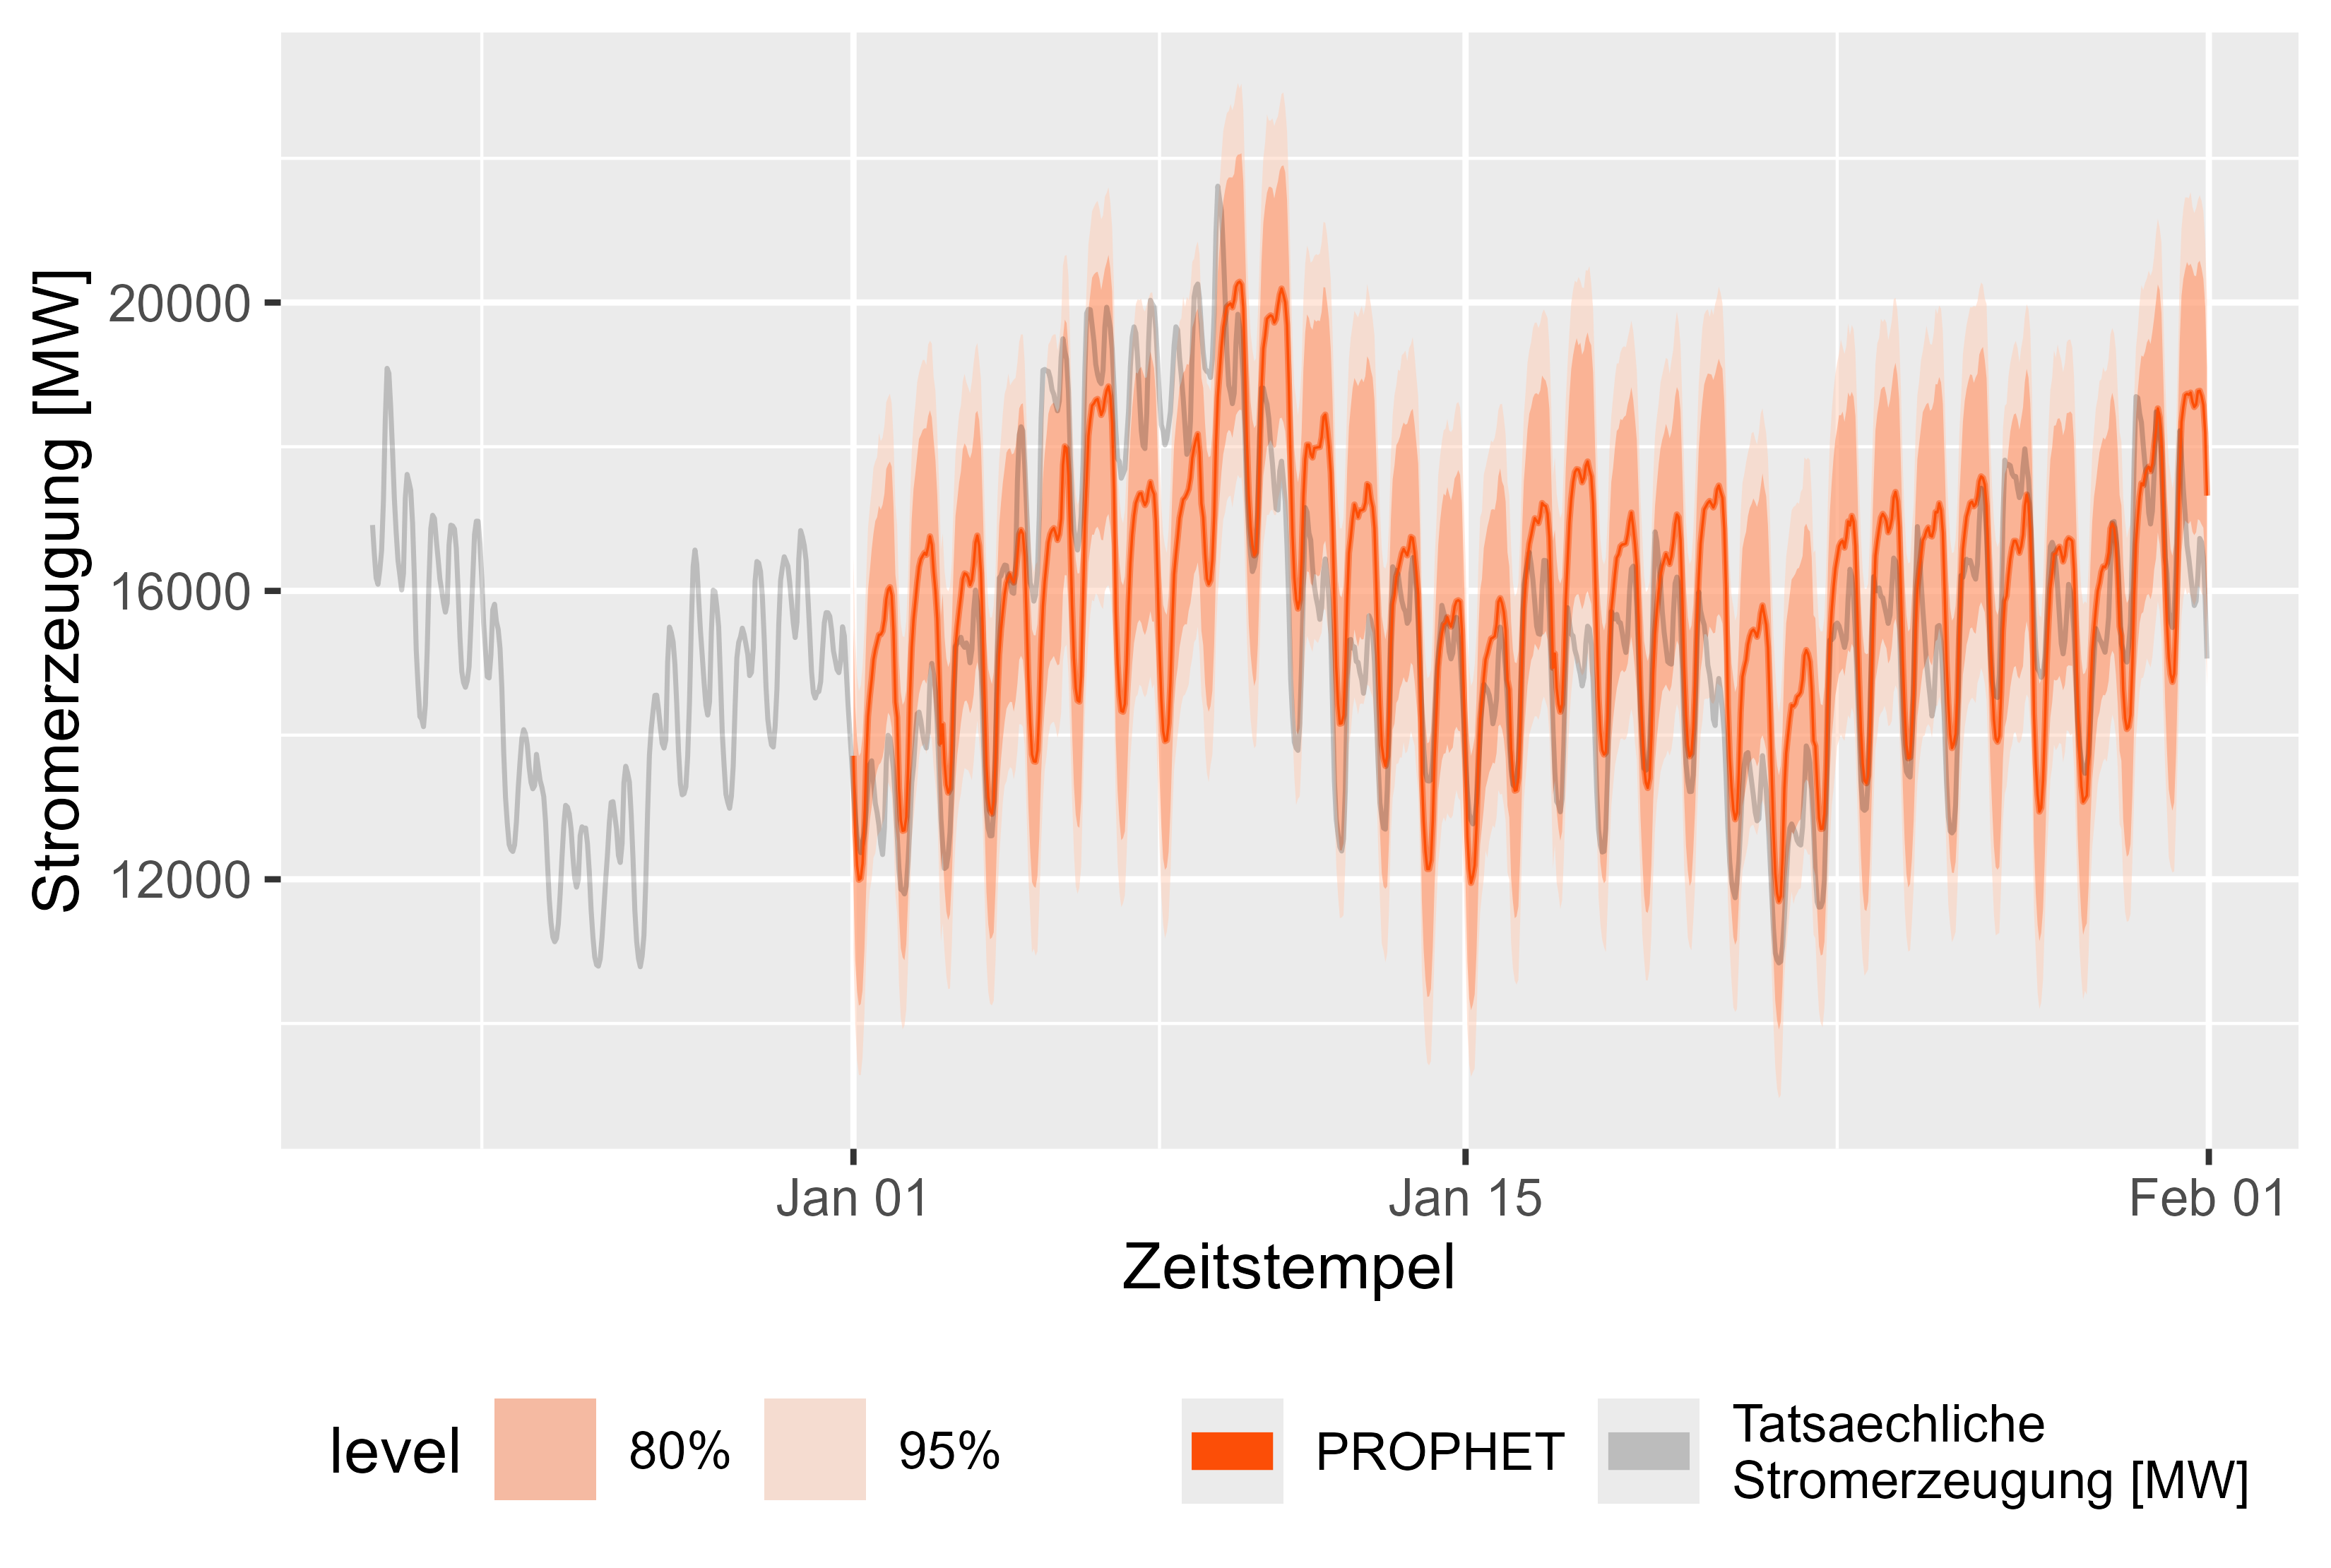
\includegraphics[width=1.0\textwidth]{plots/statistic_approach_PROPHET.png}
\caption{Prophet, Ausschnitt für Januar}
\label{fig:prophet_january}
\end{figure}

Die Abbildung \ref{fig:prophet_real_sim} stellt die Vorhersage gegenüber den realen Beobachtungen dar. Deutlich zu erkennen, dass die Vorhersage werte für das Prophet-Modell sich um die schwarze Gerade streuen. Diese Gerade soll eine perfekte Vorhersage darstellen. Die Streuung um diese Gerade kann auch als Residueen angesehen werden.

\begin{figure}[H]
\centering
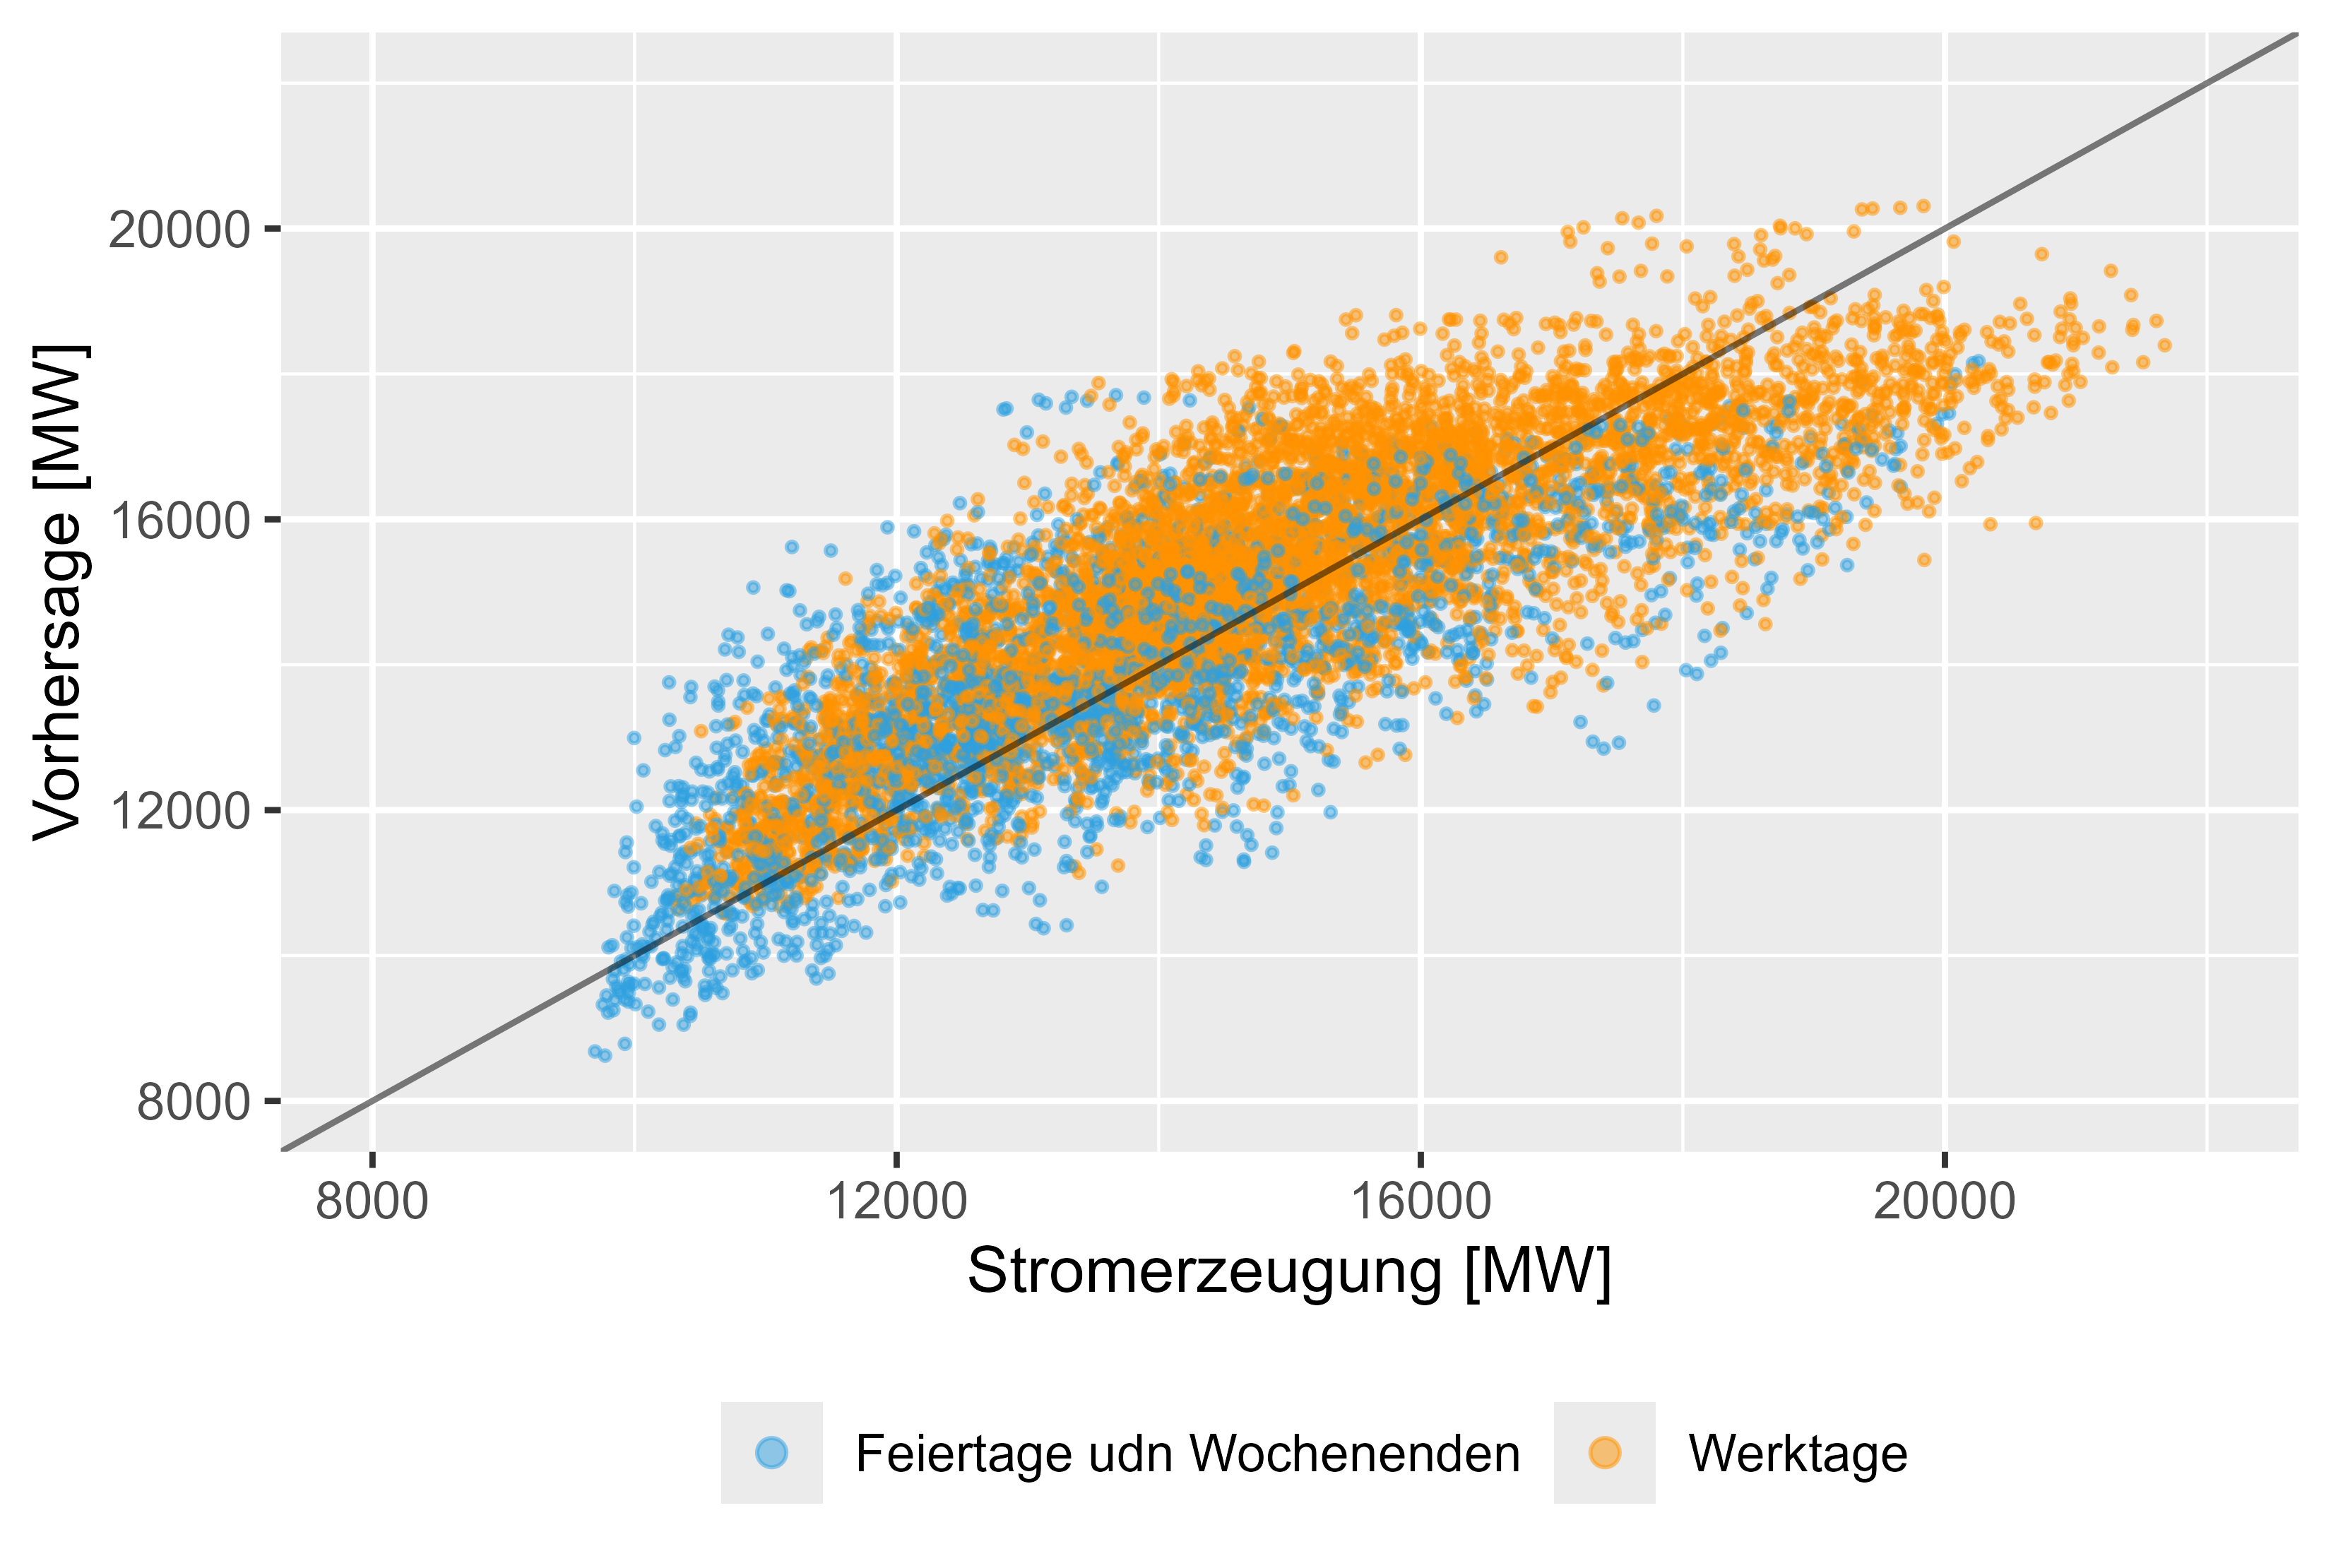
\includegraphics[width=1.0\textwidth]{plots/real_to_fc_statistic_approach_PROPHET.png}
\caption{Prophet, Vorhersage gegenüber realen Beobachtungen}
\label{fig:prophet_real_sim}
\end{figure}

Das neuronale Netz ist mit einem MAPE von 6.62\% besser als das Prophet-Modell. Dabei ist zwischen ``LNN mit SLAF'' und ``LNN'' zu unterscheiden. LNN mit SLAF konnte leider nicht so gut performen wie LNN (ohne SLAF). Ein Grund dafür kann z.B. sein, dass das LNN nicht für ein SLAF geeignet ist, oder dass SLAF für Zeitreihen nicht anwendbar ist. Die Abbildung \ref{fig:slaf_lnn_100_epochs_january} zeigt die Vorhersage für den Januar 2017 nach 100 Epochen. Hier wird gezeigt, dass LNN sich besser an das saisonale Muster anpassen kann als ein LNN mit SLAF. LNN mit SLAF hat zwar an einigen Stellen das Muster erkennen können, aber nicht über den ganzen Datensatz hinweg.

\begin{figure}[H]
\centering
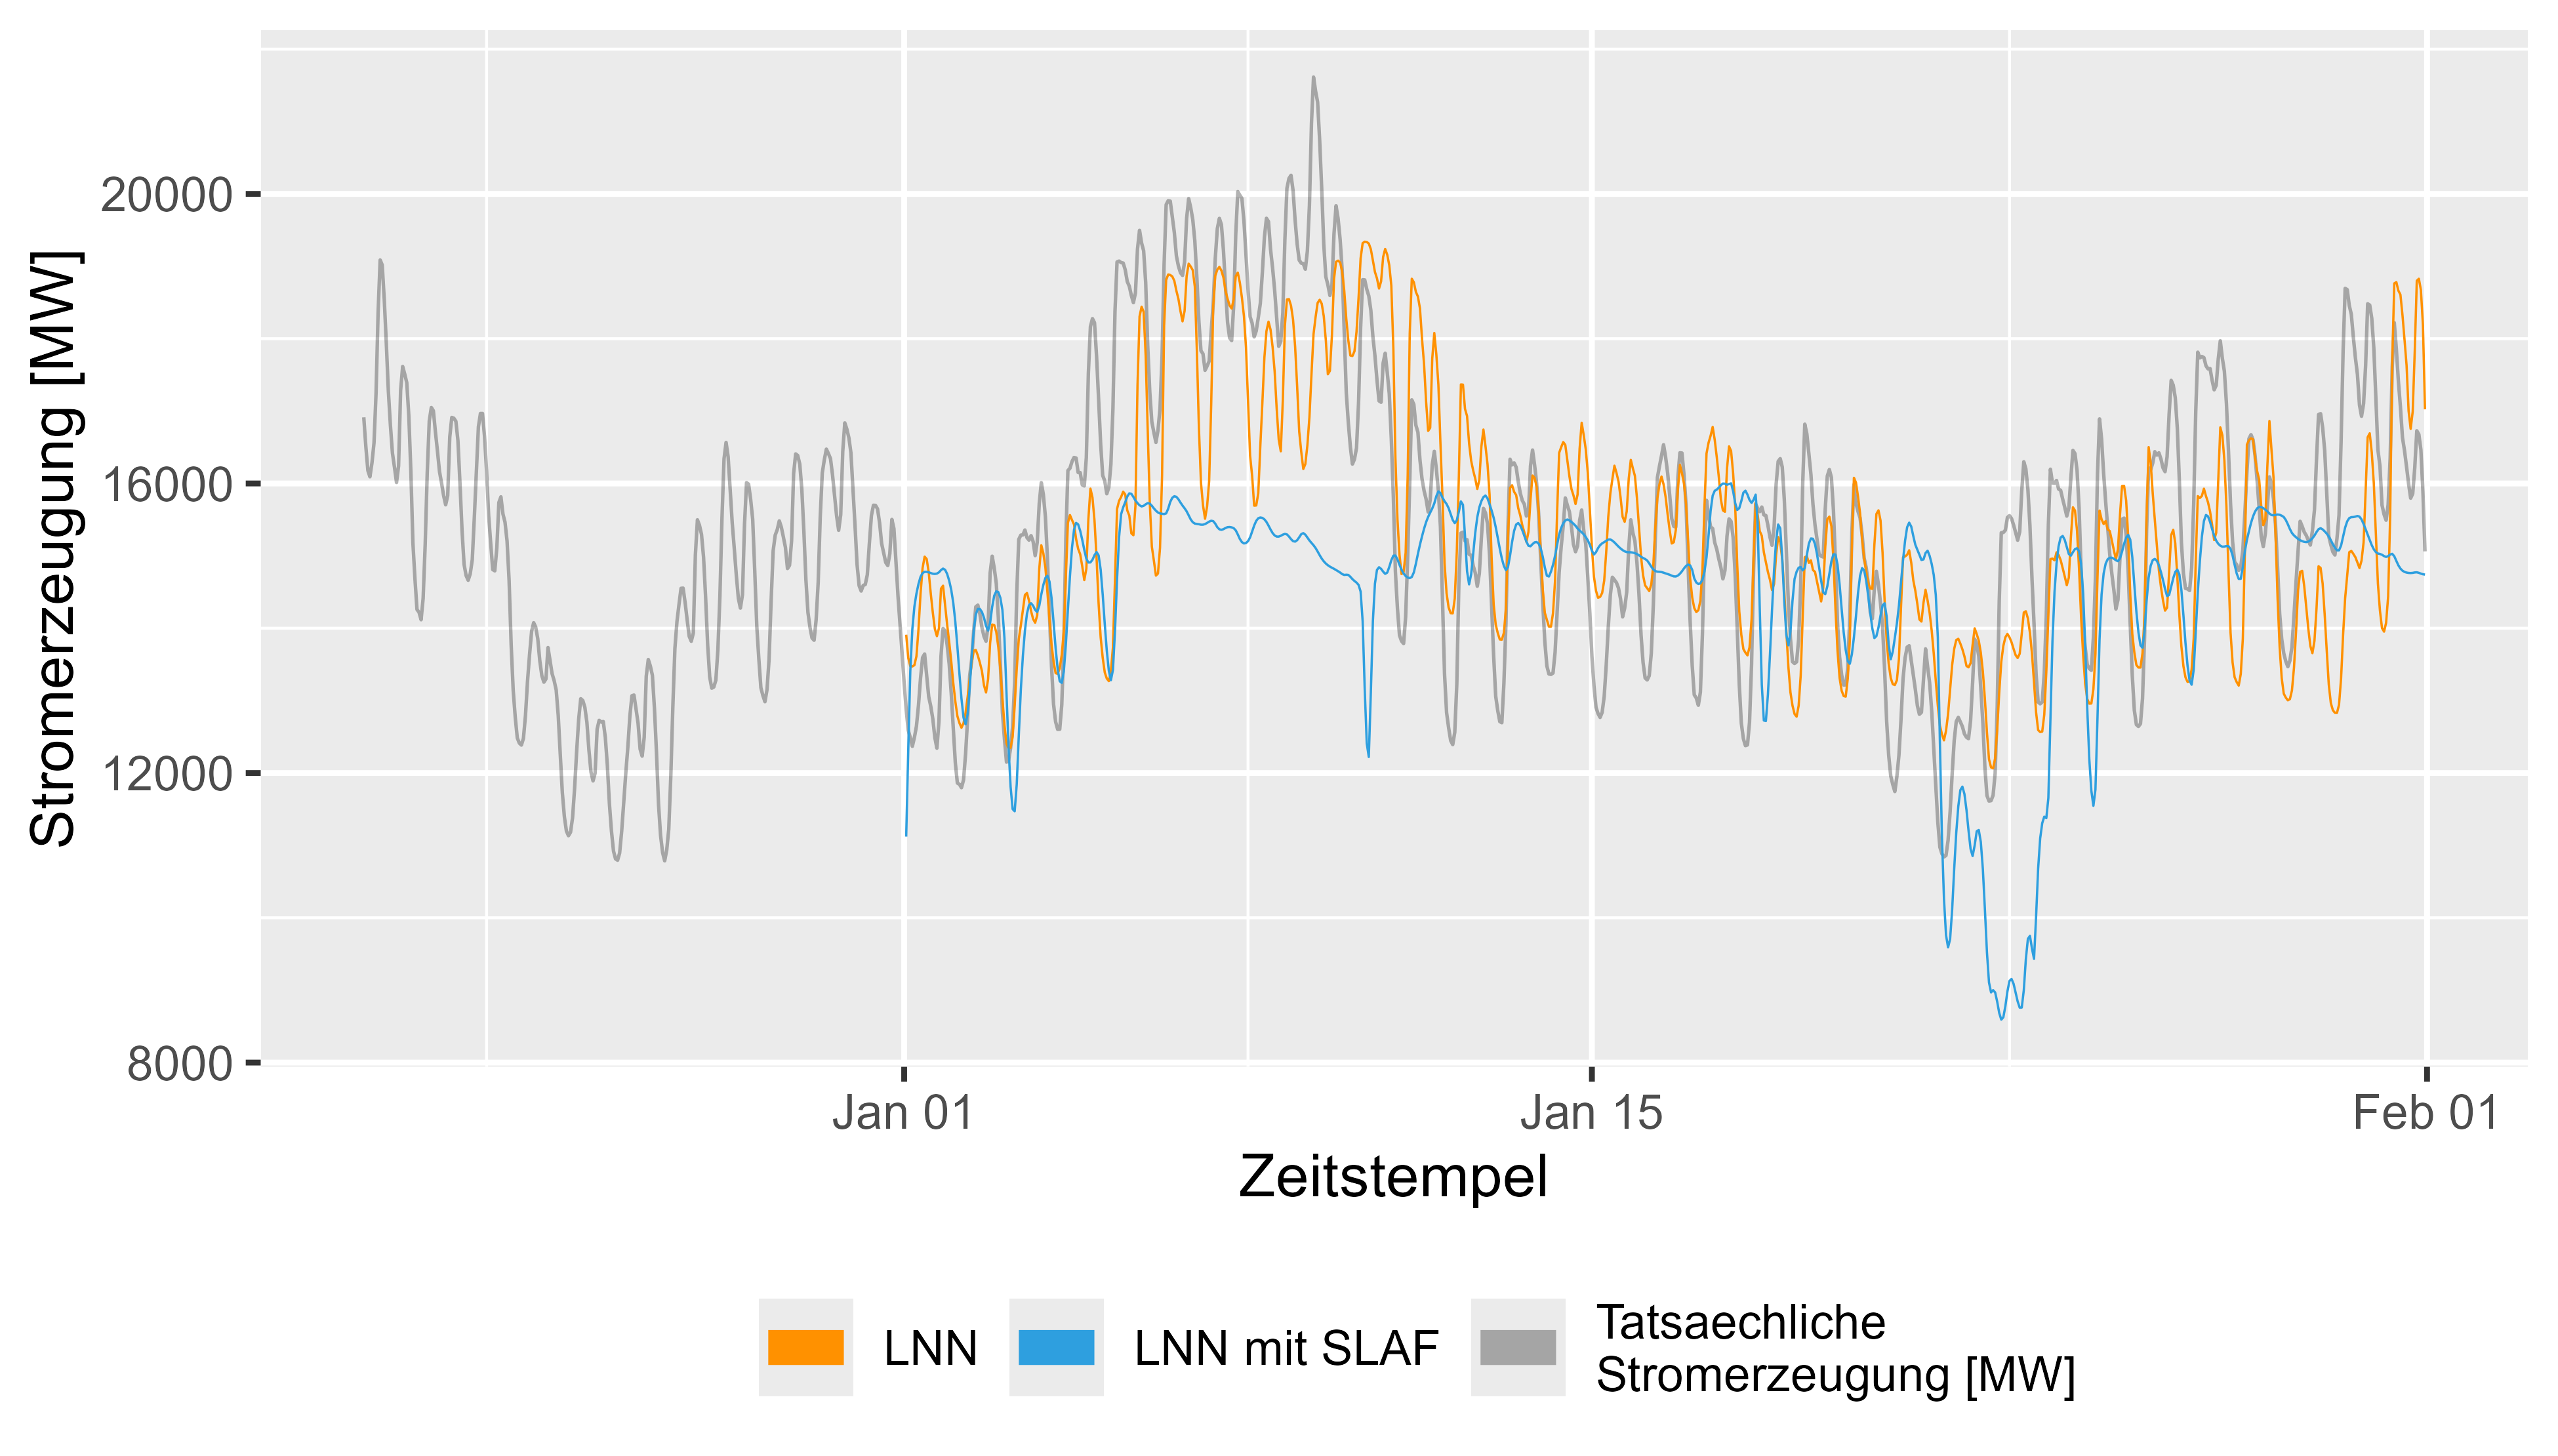
\includegraphics[width=1.0\textwidth]{plots/cobmined_nnLNN.png}
\caption{Nach 100 Epochen mit und ohne SLAF, Ausschnitt für Januar}
\label{fig:slaf_lnn_100_epochs_january}
\end{figure}

Auch in der Jahresbetrachtung sieht LNN begründet aus. LNN passt sich an das moustache-Muster über das ganze Jahr sehr gut an
und ist damit auch für eine Vorhersage von Stromerzeugung bzw. von Zeitreihen geeignet. LNN mit SLAF war in dem Fall nicht so erfolgreich. Zwar folgt es halbwegs dem Verlauf, erkennt aber das saisonale Muster nicht so gut wie LNN ohne SLAF. Die Abbildung \ref{fig:slaf_lnn_100_epochs_2017} zeigt dabei die Vorhersage der beiden Modelle für das Jahr 2017 nach 100 Epochen.

\begin{figure}[H]
\centering
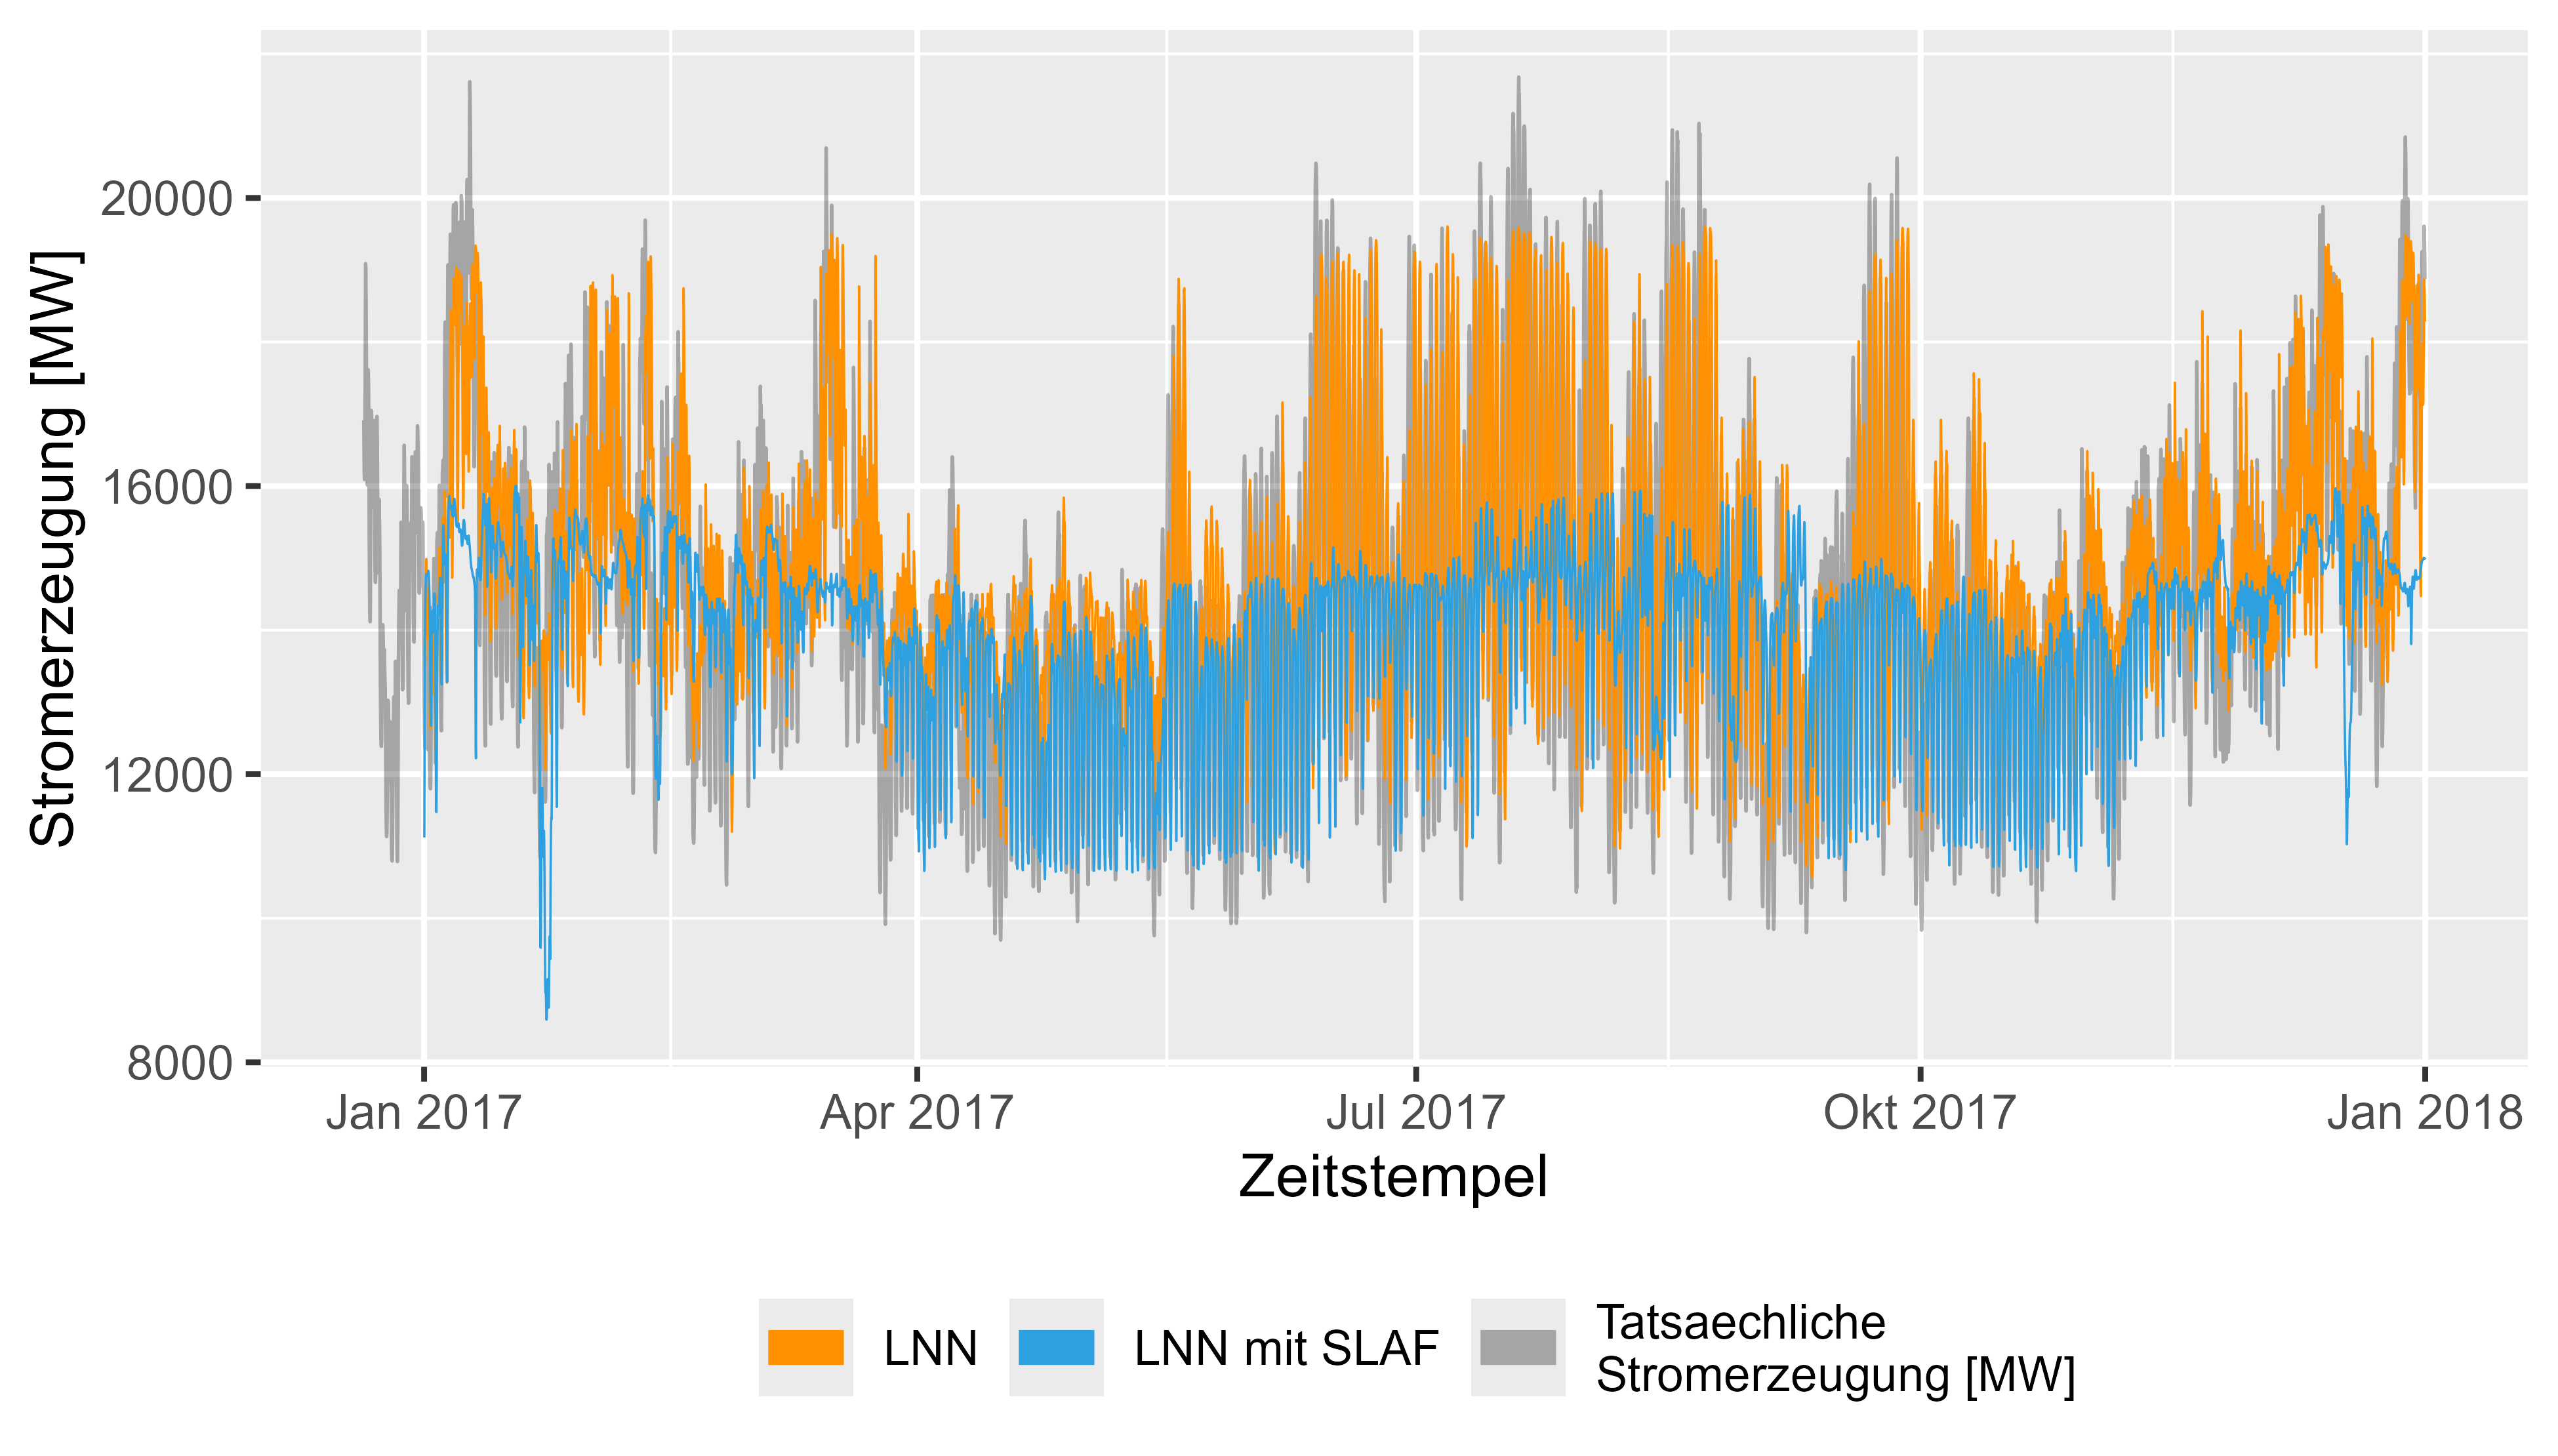
\includegraphics[width=1.0\textwidth]{plots/all_time_cobmined_nnLNN.png}
\caption{Nach 100 Epochen mit und ohne SLAF, ganzes Jahr 2017}
\label{fig:slaf_lnn_100_epochs_2017}
\end{figure}

Der Vergleich zwischen Abbildung \ref{fig:prophet_real_sim} und \ref{fig:slaf_lnn_100_epochs_lnn} zeigt, dass beim LNN ein ähnliches Muster entsteht wie beim Prophet Modell für die Vorhersage werte gegenüber den echten Beobachtungen. Anzumerken hier ist, dass LNN eine künstliche Grenze im oberen Bereich gezogen hat. Diese Grenze konnte mit Normalisierung zwar gedämmt werden, konnte jedoch nicht komplett aufgelöst werden. Dies zeigt, dass LNNs noch mehr Potenzial haben kann. Wobei das LNN noch weiter optimiert werden muss.

\begin{figure}[H]
\centering
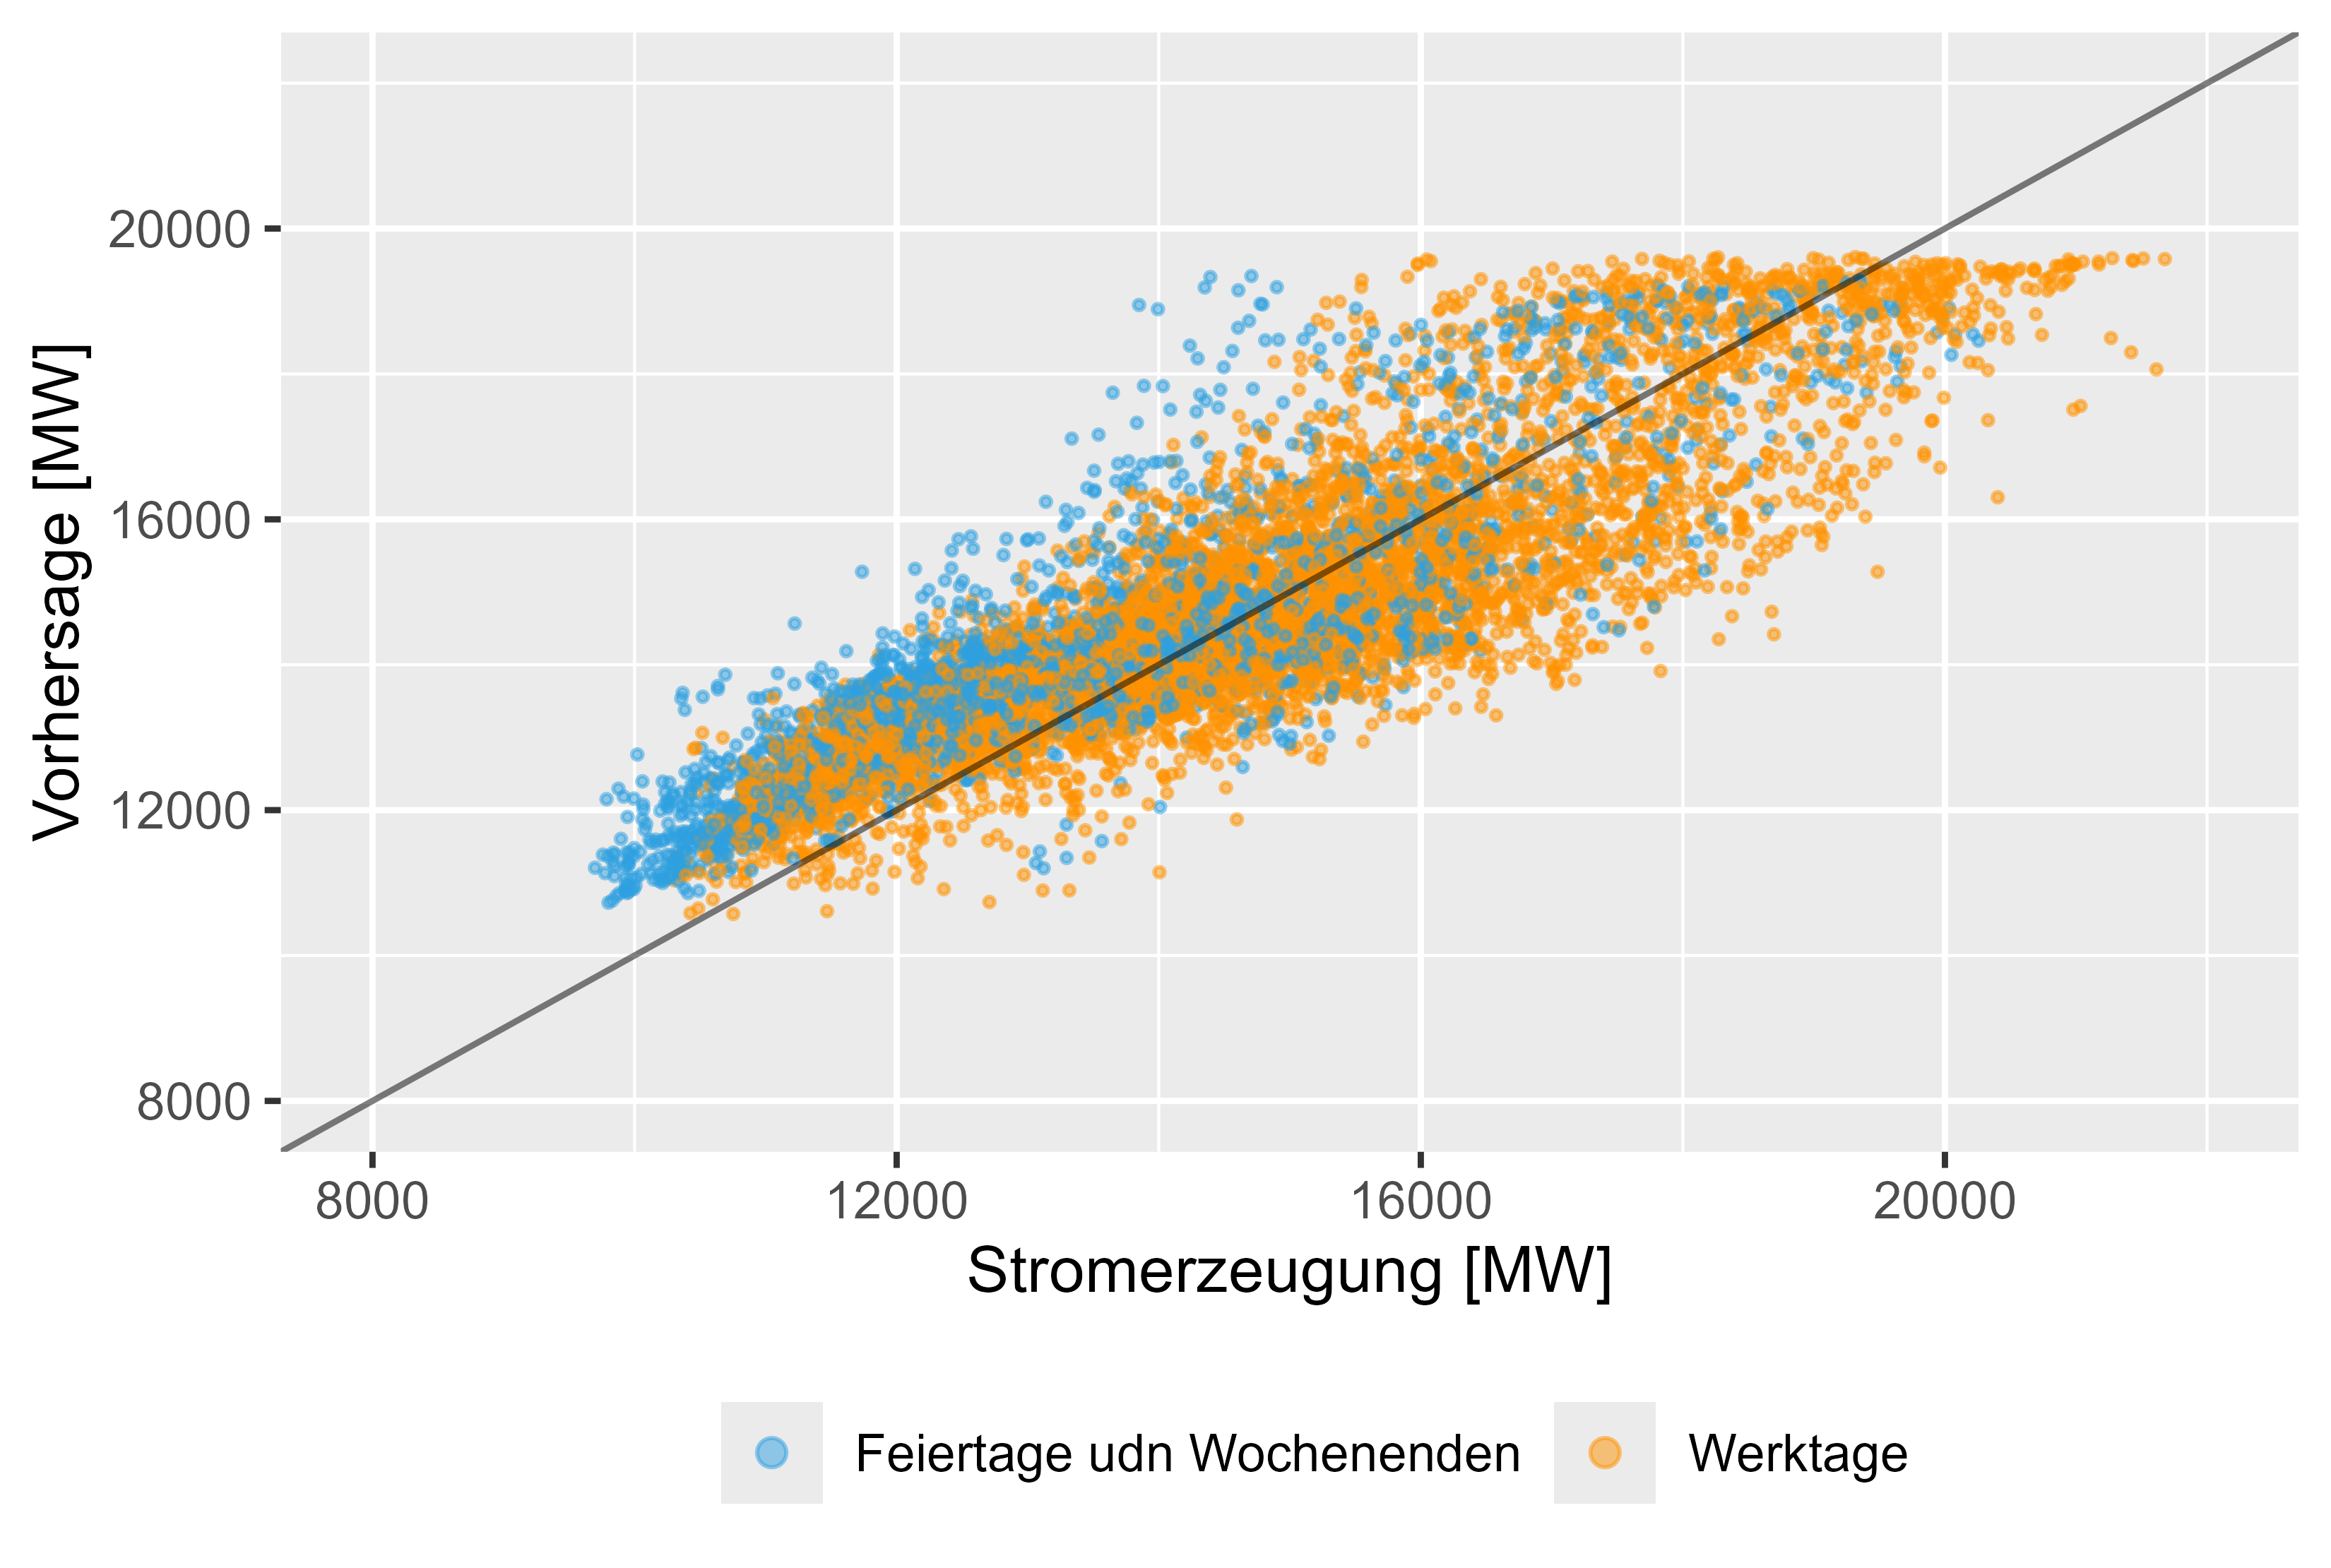
\includegraphics[width=1.0\textwidth]{plots/real_to_fc_all_time_cobmined_nnLNN.png}
\caption{Nach 100 Epochen LNN, Vorhersage gegenüber realen Beobachtungen}
\label{fig:slaf_lnn_100_epochs_lnn}
\end{figure}

LNN mit SLAF in Abbildung \ref{fig:slaf_lnn_100_epochs_lnn_slaf} sieht im Gegensatz dazu nicht so gut aus. LNN mit SLAF hat eine stärkere Unter- und Obergrenze gezogen. Die Datenwolke ist konzentrierter und breiter um die perfekte Vorhersage gestreut. Wieder deutlich, dass LNN mit SLAF nicht so gut geeignet ist wie LNN ohne SLAF.

\begin{figure}[H]
\centering
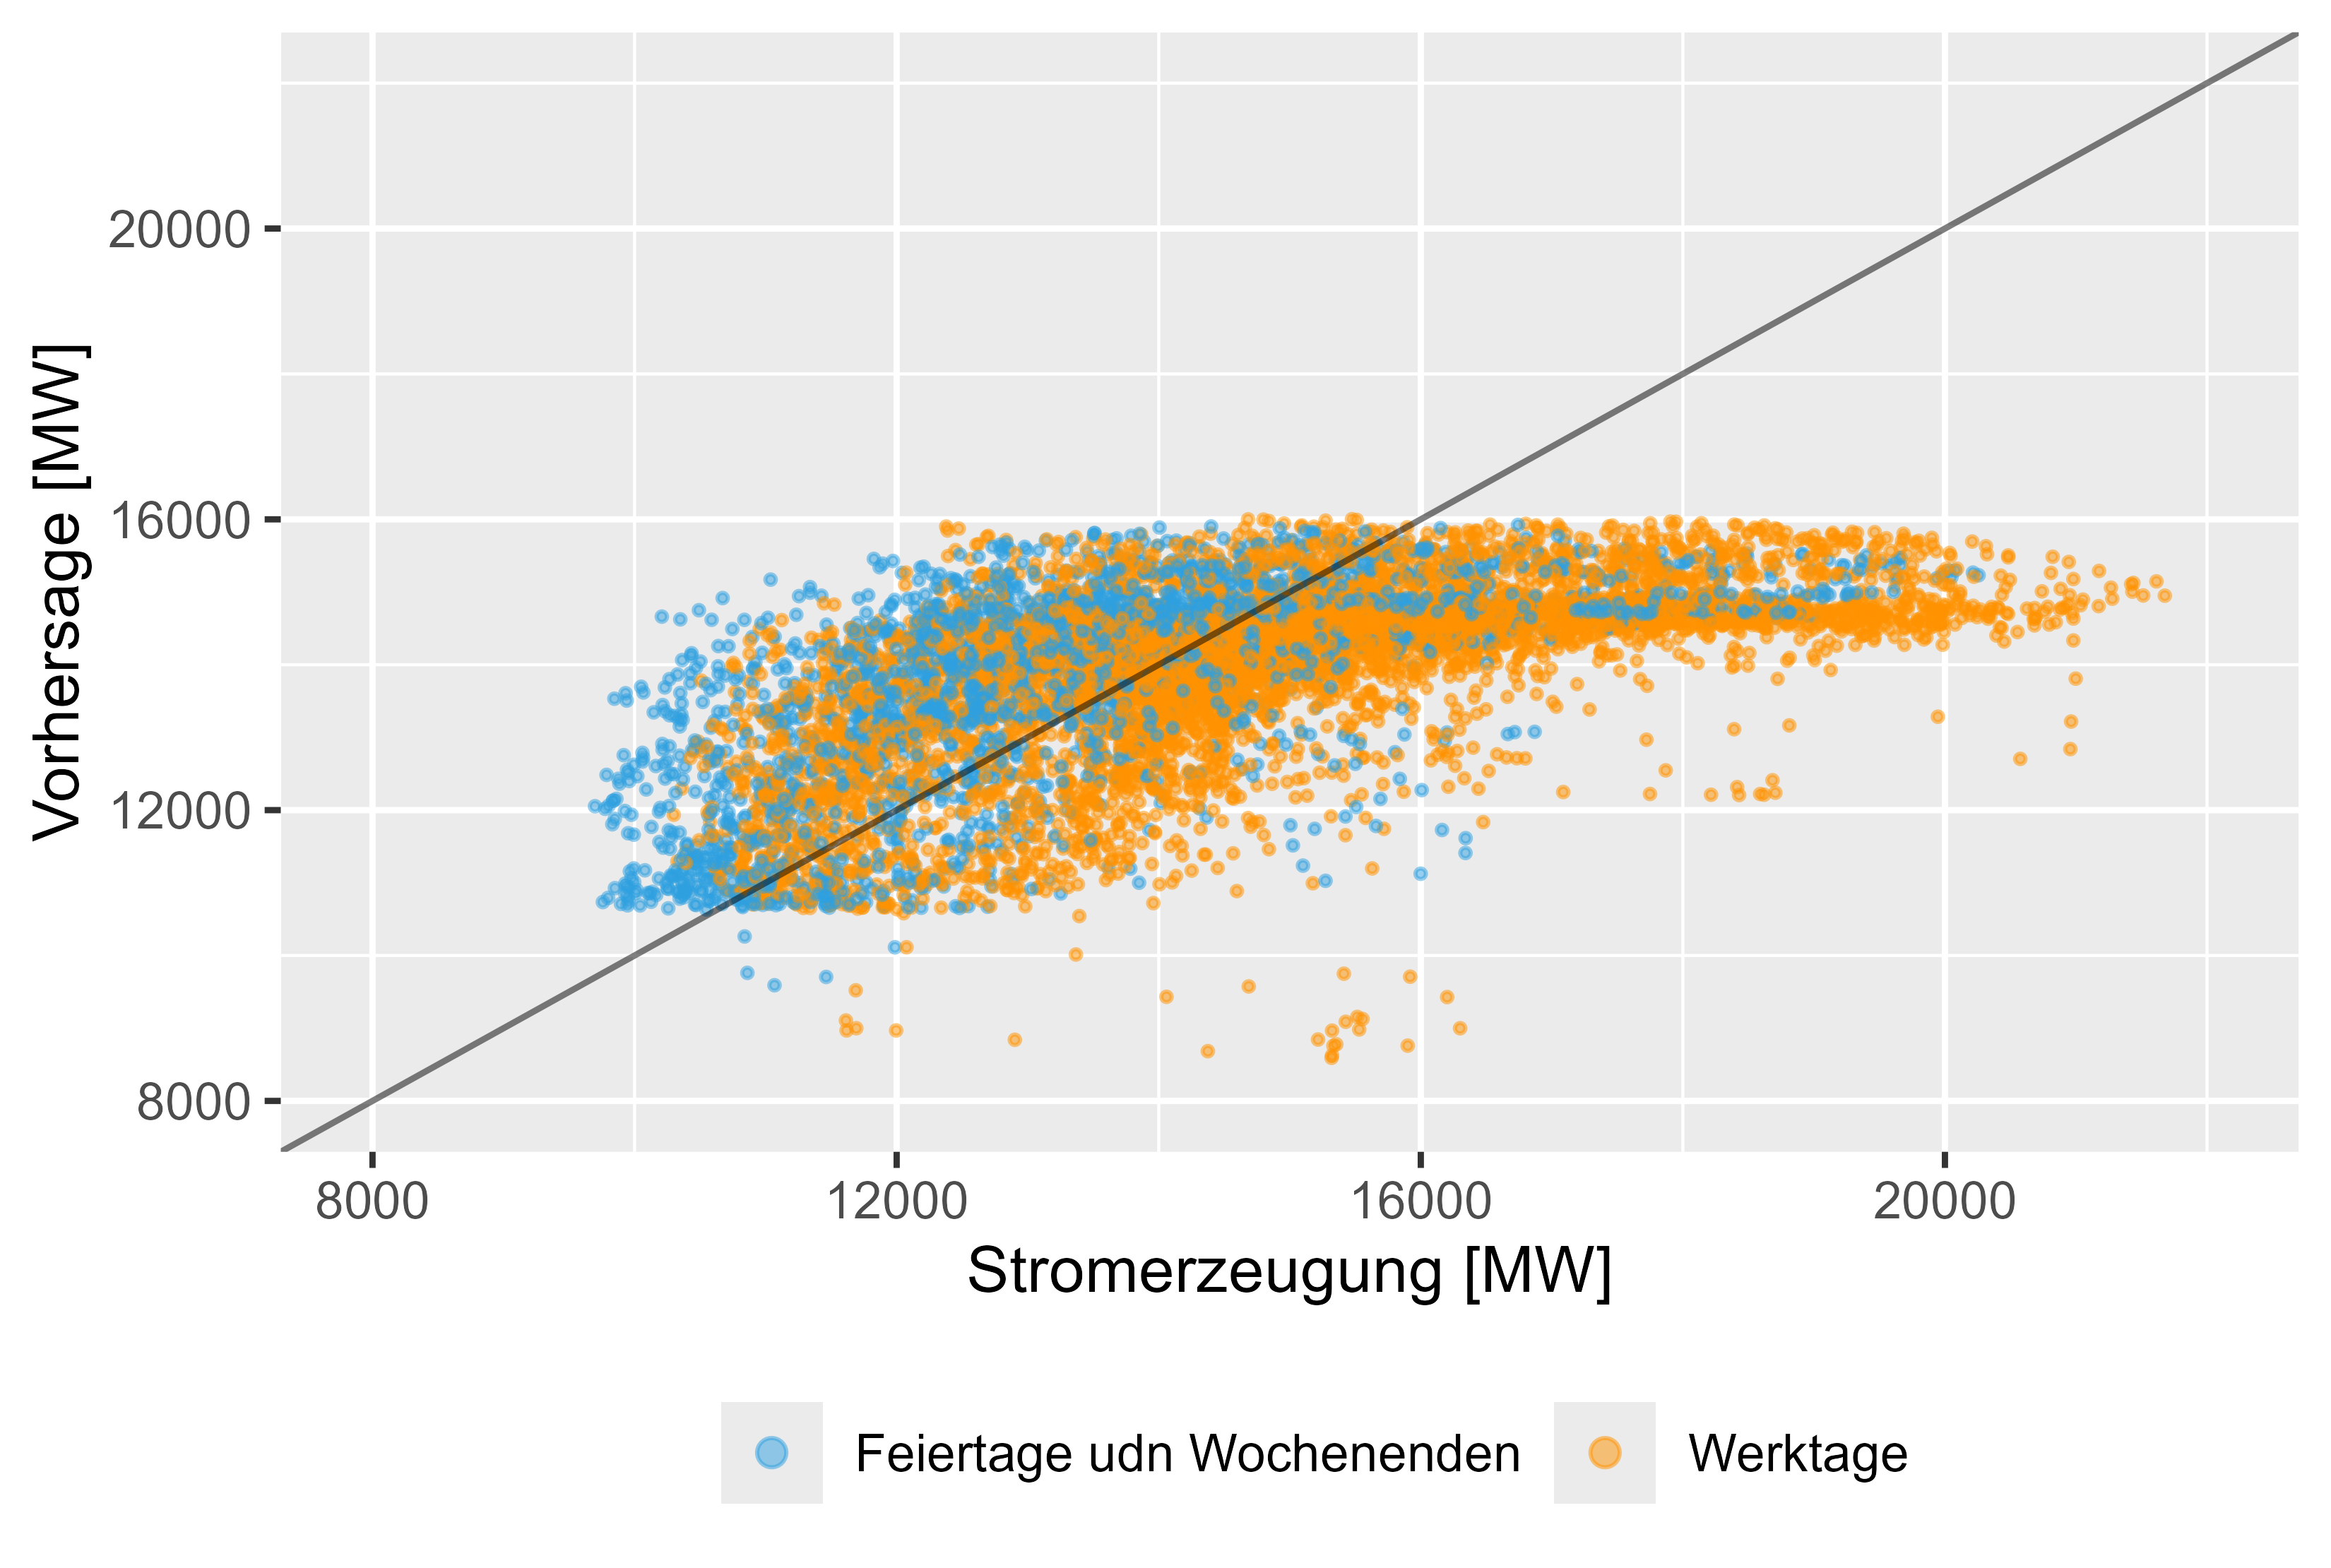
\includegraphics[width=0.8\textwidth]{plots/real_to_fc_cobmined_nnLNN mit SLAF.png}
\caption{Nach 100 Epochen LNN + SLAF, Vorhersage gegenüber realen Beobachtungen}
\label{fig:slaf_lnn_100_epochs_lnn_slaf}
\end{figure}

Die Trainings-Verluste zeigen jedoch, dass im Training sich LNN mit SLAF an den Verlust vom Training ohne SLAF annähert. Genau dieses Verhalten war auch zu erwarten, da SLAFs mit swish nur eine Approximation der echten ReLU-Funktion ist.

\begin{figure}[H]
\centering
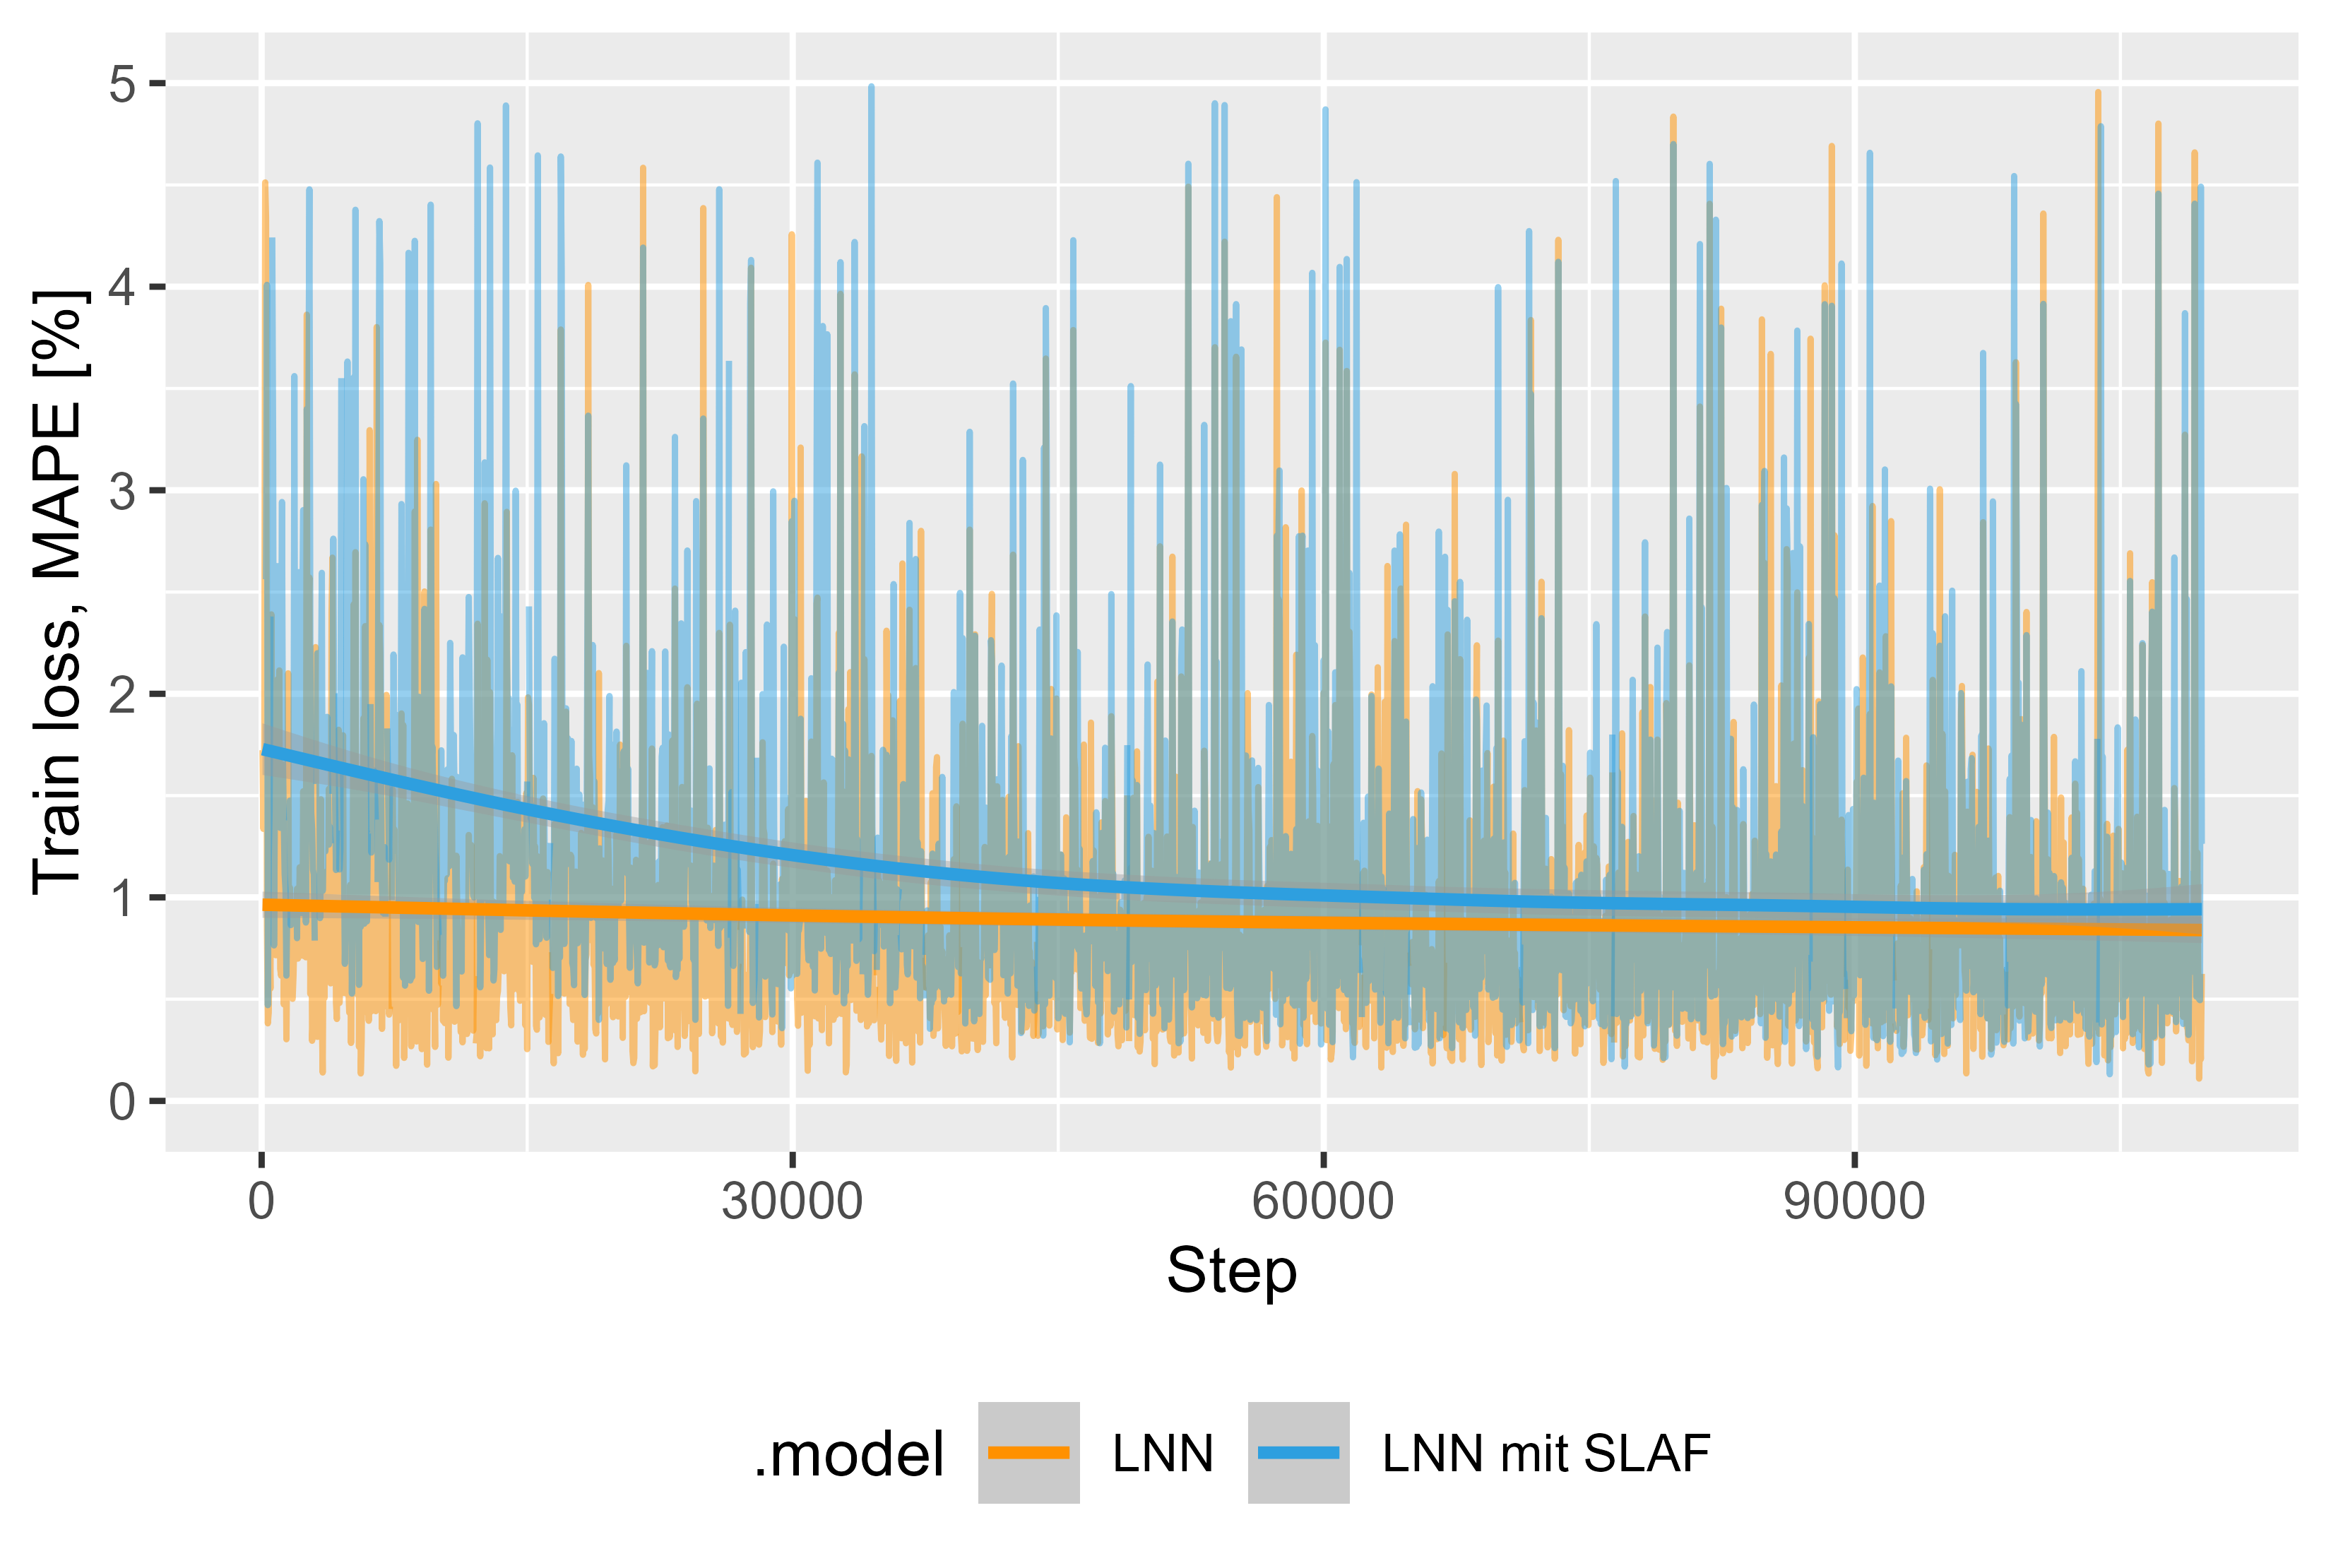
\includegraphics[width=0.8\textwidth]{plots/training_loss.png}
\caption{MAPE Verlust in den einzelnen Schritten (eine Epoche sind mehrere Schritte)}
\label{fig:train_loss}
\end{figure}

\clearpage
\newpage

Die Tabelle \ref{table:model_comparison} fasst nochmal alle Ergebnisse zusammen. Wie besprochen ist LNN mit einem MAPE von 6.62\% ein sehr gutes Ergebnisss für die Stromerzeugung und geeignet für eine Vorhersage. Anzumerken ist hier, dass das ARIMA Modell und das Prophet-Modell nicht optimiert wurden. Ebenfalls konnte LNN nicht vollständig durch die enorme Trainingszeit (2 Studen ca. für 100 Epochen) optimiert werden.

\begin{table}[h!]
\centering
\begin{tabular}{|c|l|c|c|c|}
\hline
\textbf{Nr.} & \textbf{Model}              & \textbf{RMSE}    & \textbf{MAPE}    & \textbf{MAE}     \\ \hline
1            & LNN                         & 1170         & 6.62         & 937         \\ \hline
2            & PROPHET                     & 1351         & 7.49         & 1071        \\ \hline
3            & ARIMA                       & 1421         & 7.68         & 1118        \\ \hline
4            & LNN mit SLAF                & 1895         & 9.63        & 1443        \\ \hline
5            & NAIVE                       & 2423         & 12.60        & 1887        \\ \hline
6            & DRIFT                       & 2592         & 13.26        & 2025        \\ \hline
7            & MEAN                        & 2322         & 13.72        & 1888        \\ \hline
8            & LNN mit SLAF 10 Epochen     & 3721         & 19.83        & 2865        \\ \hline
9            & LNN 10 Epochen              & 3779         & 23.57        & 3307        \\ \hline
\end{tabular}
\caption{Vergleich der Modelle mit RMSE, MAPE und MAE}
\label{table:model_comparison}
\end{table}

\clearpage
\newpage

\section{Fazit}\label{fazit}

In dieser Arbeit wurde gezeigt, dass LNNs ohne SLAF für eine Vorhersage von Zeitreihen im Bereich der Energiewirtschaft geeignet sind. Durch eine umfassende Datenanalyse konnten die notwendigen Features für die Modellierung extrahiert werden. Der Vergleich zu den herkömmlichen statistischen Modellen zeigt ein großes Potenzial im Bereich von Zeitreihen für LNNs auf. Schon in wenigen Schritten kann ein LNN so optimiert werden, dass es ein unoptimiertes statistisches Modell übertrumpft. Die saisonalen Muster werden genauso gut von dem LNN erkannt wie von einem statistischen Modell. Der einzige Nachteil eines LNNs gegenüber einem statistischen Modell sind die Vorhersageintervalle.

Diese werden bei einem LNN nicht automatisch mit erzeugt, können jedoch durch weitere Verfahren ermittelt und für LNNs angepasst werden (Forschungsfrage). LNNs mit SLAF performen zwar nicht so gut, können aber vielleicht weiter angepasst werden. Denn LNNs sind von Grund auf nicht für SLAF optimiert worden. Dabei könnte eine weitere Forschungsfrage entstehen und zwar wie SLAF am besten für LNNs optimiert werden kann und welche Vorteile das dann mit sich bringt.

Im Großen und Ganzen sollten LNNs im Bereich der Zeitreihen weiter untersucht werden und tiefergehende Modellierungen und Optimierungen erzeugt werden.

\newpage
\printbibliography

\end{document}
